% Options for packages loaded elsewhere
\PassOptionsToPackage{unicode}{hyperref}
\PassOptionsToPackage{hyphens}{url}
\PassOptionsToPackage{dvipsnames,svgnames*,x11names*}{xcolor}
%
\documentclass[
  11pt,
]{article}
\usepackage[]{mathpazo}
\usepackage{amssymb,amsmath}
\usepackage{ifxetex,ifluatex}
\ifnum 0\ifxetex 1\fi\ifluatex 1\fi=0 % if pdftex
  \usepackage[T1]{fontenc}
  \usepackage[utf8]{inputenc}
  \usepackage{textcomp} % provide euro and other symbols
\else % if luatex or xetex
  \usepackage{unicode-math}
  \defaultfontfeatures{Scale=MatchLowercase}
  \defaultfontfeatures[\rmfamily]{Ligatures=TeX,Scale=1}
\fi
% Use upquote if available, for straight quotes in verbatim environments
\IfFileExists{upquote.sty}{\usepackage{upquote}}{}
\IfFileExists{microtype.sty}{% use microtype if available
  \usepackage[]{microtype}
  \UseMicrotypeSet[protrusion]{basicmath} % disable protrusion for tt fonts
}{}
\makeatletter
\@ifundefined{KOMAClassName}{% if non-KOMA class
  \IfFileExists{parskip.sty}{%
    \usepackage{parskip}
  }{% else
    \setlength{\parindent}{0pt}
    \setlength{\parskip}{6pt plus 2pt minus 1pt}}
}{% if KOMA class
  \KOMAoptions{parskip=half}}
\makeatother
\usepackage{xcolor}
\IfFileExists{xurl.sty}{\usepackage{xurl}}{} % add URL line breaks if available
\IfFileExists{bookmark.sty}{\usepackage{bookmark}}{\usepackage{hyperref}}
\hypersetup{
  pdftitle={Data Science Project Guide: Covid-19},
  pdfauthor={TechAcademy e.V.},
  colorlinks=true,
  linkcolor=Maroon,
  filecolor=Maroon,
  citecolor=Blue,
  urlcolor=blue,
  pdfcreator={LaTeX via pandoc}}
\urlstyle{same} % disable monospaced font for URLs
\usepackage[top=0.5in, bottom=1.5in, left=1in, right=1in, a4paper]{geometry}
\usepackage{color}
\usepackage{fancyvrb}
\newcommand{\VerbBar}{|}
\newcommand{\VERB}{\Verb[commandchars=\\\{\}]}
\DefineVerbatimEnvironment{Highlighting}{Verbatim}{commandchars=\\\{\}}
% Add ',fontsize=\small' for more characters per line
\usepackage{framed}
\definecolor{shadecolor}{RGB}{248,248,248}
\newenvironment{Shaded}{\begin{snugshade}}{\end{snugshade}}
\newcommand{\AlertTok}[1]{\textcolor[rgb]{0.94,0.16,0.16}{#1}}
\newcommand{\AnnotationTok}[1]{\textcolor[rgb]{0.56,0.35,0.01}{\textbf{\textit{#1}}}}
\newcommand{\AttributeTok}[1]{\textcolor[rgb]{0.77,0.63,0.00}{#1}}
\newcommand{\BaseNTok}[1]{\textcolor[rgb]{0.00,0.00,0.81}{#1}}
\newcommand{\BuiltInTok}[1]{#1}
\newcommand{\CharTok}[1]{\textcolor[rgb]{0.31,0.60,0.02}{#1}}
\newcommand{\CommentTok}[1]{\textcolor[rgb]{0.56,0.35,0.01}{\textit{#1}}}
\newcommand{\CommentVarTok}[1]{\textcolor[rgb]{0.56,0.35,0.01}{\textbf{\textit{#1}}}}
\newcommand{\ConstantTok}[1]{\textcolor[rgb]{0.00,0.00,0.00}{#1}}
\newcommand{\ControlFlowTok}[1]{\textcolor[rgb]{0.13,0.29,0.53}{\textbf{#1}}}
\newcommand{\DataTypeTok}[1]{\textcolor[rgb]{0.13,0.29,0.53}{#1}}
\newcommand{\DecValTok}[1]{\textcolor[rgb]{0.00,0.00,0.81}{#1}}
\newcommand{\DocumentationTok}[1]{\textcolor[rgb]{0.56,0.35,0.01}{\textbf{\textit{#1}}}}
\newcommand{\ErrorTok}[1]{\textcolor[rgb]{0.64,0.00,0.00}{\textbf{#1}}}
\newcommand{\ExtensionTok}[1]{#1}
\newcommand{\FloatTok}[1]{\textcolor[rgb]{0.00,0.00,0.81}{#1}}
\newcommand{\FunctionTok}[1]{\textcolor[rgb]{0.00,0.00,0.00}{#1}}
\newcommand{\ImportTok}[1]{#1}
\newcommand{\InformationTok}[1]{\textcolor[rgb]{0.56,0.35,0.01}{\textbf{\textit{#1}}}}
\newcommand{\KeywordTok}[1]{\textcolor[rgb]{0.13,0.29,0.53}{\textbf{#1}}}
\newcommand{\NormalTok}[1]{#1}
\newcommand{\OperatorTok}[1]{\textcolor[rgb]{0.81,0.36,0.00}{\textbf{#1}}}
\newcommand{\OtherTok}[1]{\textcolor[rgb]{0.56,0.35,0.01}{#1}}
\newcommand{\PreprocessorTok}[1]{\textcolor[rgb]{0.56,0.35,0.01}{\textit{#1}}}
\newcommand{\RegionMarkerTok}[1]{#1}
\newcommand{\SpecialCharTok}[1]{\textcolor[rgb]{0.00,0.00,0.00}{#1}}
\newcommand{\SpecialStringTok}[1]{\textcolor[rgb]{0.31,0.60,0.02}{#1}}
\newcommand{\StringTok}[1]{\textcolor[rgb]{0.31,0.60,0.02}{#1}}
\newcommand{\VariableTok}[1]{\textcolor[rgb]{0.00,0.00,0.00}{#1}}
\newcommand{\VerbatimStringTok}[1]{\textcolor[rgb]{0.31,0.60,0.02}{#1}}
\newcommand{\WarningTok}[1]{\textcolor[rgb]{0.56,0.35,0.01}{\textbf{\textit{#1}}}}
\usepackage{longtable,booktabs}
% Correct order of tables after \paragraph or \subparagraph
\usepackage{etoolbox}
\makeatletter
\patchcmd\longtable{\par}{\if@noskipsec\mbox{}\fi\par}{}{}
\makeatother
% Allow footnotes in longtable head/foot
\IfFileExists{footnotehyper.sty}{\usepackage{footnotehyper}}{\usepackage{footnote}}
\makesavenoteenv{longtable}
\usepackage{graphicx}
\makeatletter
\def\maxwidth{\ifdim\Gin@nat@width>\linewidth\linewidth\else\Gin@nat@width\fi}
\def\maxheight{\ifdim\Gin@nat@height>\textheight\textheight\else\Gin@nat@height\fi}
\makeatother
% Scale images if necessary, so that they will not overflow the page
% margins by default, and it is still possible to overwrite the defaults
% using explicit options in \includegraphics[width, height, ...]{}
\setkeys{Gin}{width=\maxwidth,height=\maxheight,keepaspectratio}
% Set default figure placement to htbp
\makeatletter
\def\fps@figure{htbp}
\makeatother
\setlength{\emergencystretch}{3em} % prevent overfull lines
\providecommand{\tightlist}{%
  \setlength{\itemsep}{0pt}\setlength{\parskip}{0pt}}
\setcounter{secnumdepth}{5}
\newcommand{\sectionbreak}{\clearpage}
\usepackage{booktabs}
\RequirePackage{fix-cm}
\usepackage[many]{tcolorbox}
\usepackage{xcolor}

\definecolor{r}{HTML}{2369bd}
\definecolor{p}{HTML}{ffde4d}
\definecolor{boxgrey}{HTML}{fefefe}

\newtcolorbox{rbox}{
  colback=boxgrey,
  colframe=r,
  coltext=black,
  boxsep=5pt,
  arc=4pt}
  
\newtcolorbox{pbox}{
  colback=boxgrey,
  colframe=p,
  coltext=black,
  boxsep=5pt,
  arc=4pt}


\newenvironment{tips}[1]
  {
  \begin{itemize}
  \footnotesize
  \renewcommand{\labelitemi}{
    \raisebox{-.7\height}[0pt][0pt]{
      {\setkeys{Gin}{width=3em,keepaspectratio}
        \includegraphics{images/#1.png}}
    }
  }
  \setlength{\fboxsep}{1em}
  \begin{rbox}
  \item
  }
  {
  \end{rbox}
  \end{itemize}
  }
  
  
\newenvironment{tipsp}[1]
  {
  \begin{itemize}
  \footnotesize
  \renewcommand{\labelitemi}{
    \raisebox{-.7\height}[0pt][0pt]{
      {\setkeys{Gin}{width=3em,keepaspectratio}
        \includegraphics{images/#1.png}}
    }
  }
  \setlength{\fboxsep}{1em}
  \begin{pbox}
  \item
  }
  {
  \end{pbox}
  \end{itemize}
  }
  
\usepackage{fancyhdr}
\pagestyle{fancyplain}
\usepackage{setspace}
\usepackage{chngcntr}
\onehalfspacing

\usepackage{titling}
\pretitle{\begin{center}\LARGE
\includegraphics[width=6cm]{plots/TA_Logo.png}\\[\bigskipamount]}
\posttitle{\end{center}}
\usepackage{booktabs}
\usepackage{longtable}
\usepackage{array}
\usepackage{multirow}
\usepackage{wrapfig}
\usepackage{float}
\usepackage{colortbl}
\usepackage{pdflscape}
\usepackage{tabu}
\usepackage{threeparttable}
\usepackage{threeparttablex}
\usepackage[normalem]{ulem}
\usepackage{makecell}
\usepackage{xcolor}
\usepackage[]{natbib}
\bibliographystyle{apalike}

\title{Data Science Project Guide: Covid-19}
\author{TechAcademy e.V.}
\date{Summer Term 2020}

\begin{document}
\maketitle

\clearpage

\addtolength{\headheight}{17.82275pt}
\rhead{\includegraphics[height=0.5cm]{plots/TA_logo.png}}

\fancyfoot{}
\fancyfoot[R]{\thepage}
\addtolength{\headheight}{17.82275pt}

\fancyfoot[L]{Data Science Project Guide | Covid-19 | \copyright\ 2020, TechAcademy e.V.}

\renewcommand{\headrulewidth}{0.25pt}
\renewcommand{\footrulewidth}{0.25pt}

\tableofcontents
\clearpage

\hypertarget{welcome}{%
\section{Welcome!}\label{welcome}}

In the first few chapters you will be introduced to the basics of the \texttt{R} and \texttt{Python} tracks respectively and you will find helpful explanations to questions you might have in the beginning of your coding journey. There will be a quick introduction to the Data Science track so that you can get started with the project quickly. So let's get started with the basics!

In all tracks you will work on your project in small groups of fellow students. This not only helps you get the project done faster, it also helps make your results even better. Our experience shows: The different backgrounds of the members and discussing different opinions and ideas will produce the best results. Besides, it is of course more fun to work on a project together than to code alone!\\
The groups can consist of a maximum of three members. You can choose your two teammates independently, we won't interfere with your arrangements. It is important that all group members complete the same level of difficulty (beginner or advanced), since the tasks are different in scope for each level. We explicitly encourage you to collaborate with students from different departments. This not only allows you to get to know people from other departments, but may even give you a whole new perspective on the project and tasks.
When submitting it is important to note: for a certificate, each person must submit the project individually. However, this can be identical within your group. You can get more information at our first Coding Meetup on \textbf{May 20, 2020}.

Every semester, we at TechAcademy think hard about a new project that is suited for you to learn data science. This semester, the topic choice was rather straightforward. Covid-19 is the dominating issue for our society at the time of writing this project in March and April 2020. We developed this case study as the crisis was unfolding in real time. So the recency of this topic comes at a small cost to you -- the data is changing rapidly and so are the results and conclusions. Not every textbook method works perfectly well on this data set -- but that's how it is in real life. We believe that you will learn a great deal about real life Data Science with this very timely topic. Maybe even more than you would with a polished textbook case study and data set.

This case study and the associated project guide was developed and written entirely from scratch by TechAcademy's Data Science team. Lukas Jürgensmeier and Lara Zaremba developed the project in \texttt{R}, while Felix Schneider and Manuel Mair am Tinkhof developed it in \texttt{Python}. We thank Jonathan Ratschat for providing valuable feedback on earlier versions of the project.

\hypertarget{whats-data-science-and-how-do-i-do-it}{%
\section{What's Data Science and How Do I Do It?}\label{whats-data-science-and-how-do-i-do-it}}

Data science is a multi-layered field in which the use of the latest machine learning methods is only a sub-area. To get there, you'll need many steps before -- from collecting to manipulating to exploring the data. And eventually, you will need to somehow communicate your findings.

But first things first. To analyze data, it must first be obtained. You need to know where to obtain it and how to integrate it in your respective tools. The data is rarely available as it would be needed for further processing. Familiarizing yourself with the information available, cleaning it up and processing it into the desired formats that can be read by humans and machines are important steps that often make up a large part of the work.

Before the obtained data can be analyzed, the right tool must be selected and mastered: the programming language. The most often used languages for Data Science are \texttt{R}, which was explicitly developed for statistics, and \texttt{Python}, which is characterized by its additional versatility. The data scientist does not have to be a perfect software developer who masters every detail and paradigm, but the competent handling of syntax and idiosyncrasies is essential.
There are some well-developed method collections, so-called packages or libraries, which provide a lot of functionality. The use of these collections also has to be learned and mastered.
Once all of this is achieved, the data can finally be analyzed. Here too, it is important to know and understand the multitude of statistical approaches in order to be able to choose the right method for the problem at hand. The newest, best, most beautiful neural network is not always the solution for everything.\\
One step is still missing in the data science process: understanding and communicating the results. The results are often not spontaneously intuitive or sometimes even surprising. Here, the specific expertise and creativity can be played out, especially in the visualization.

\hypertarget{whats-r}{%
\subsection{What's R?}\label{whats-r}}

\texttt{R} is a programming language that was developed by statisticians in the early 1990s for use in the calculation and visualization of statistical applications. A lot has happened since then and by now, \texttt{R} is one of the most widely used programming languages in the field of data science. Code in \texttt{R} does not have to be compiled, but can be used interactively and dynamically. This makes it possible to quickly gain basic knowledge about existing data and to display it graphically.\\
\texttt{R} offers much more than just programming, but also a complete system for solving statistical problems. A large number of packages and interfaces are available, with which the functionality can be expanded and integration into other applications is made possible.

\hypertarget{rstudio-cloud}{%
\subsubsection{RStudio Cloud}\label{rstudio-cloud}}

Before you can use \texttt{R}, you usually have to install some separate programs locally on your computer. Typically, you first install a ``raw'' version of \texttt{R}. In theory, you can then already start programming. However, it is very difficult to carry out an entire project with it. That's why there is RStudio, an Integrated Development Environment (IDE) for \texttt{R}. This includes many essential features that simplify programming with \texttt{R}. Among other things, an auto-completion of your code, a nicely structured user interface and many expansion options.

Experience has shown that installing \texttt{R} and RStudio locally takes some effort. Fortunately, RStudio also has a cloud solution that eliminates these steps: RStudio Cloud. There it is possible to edit your project in exactly the same IDE in the browser without any prior installations. You can also easily switch your project from private to public and give your team an insight into your code via a link or by giving them access to the workspace directly. In this way you are able to easily exchange ideas within your team.

We will introduce RStudio Cloud and unlock access to our workspace on our first Coding Meetup. Until then, focus on learning the hard skills of programming with your courses on DataCamp. This brings us to your curriculum in the next section.

\hypertarget{curriculum}{%
\subsubsection{Curriculum}\label{curriculum}}

The following list shows the required DataCamp courses for the Data Science with \texttt{R} Track. As a beginner, please stick to the courses of the ``beginner'' program, ambitious beginners can of course also take the advanced courses afterwards. However, the courses should be worked through in the order in which they are listed.\\
The same applies to the advanced courses. Here, too, the specified courses should be processed in the given order. Since it can of course happen that you have already mastered the topics of an advanced course, individual courses can be replaced. The topics of the advanced courses are given in key points. If these key points seem familiar to you, then take a look at the table of contents of the corresponding DataCamp course. If you are convinced that this course does not provide any added value for you, it can be replaced by one of the courses in the ``Exchange Pool'' (see list). However, this exchange course should not be processed until all other courses in the advanced course have been completed.

Both beginners and advanced learners must have completed at least two thirds of the curriculum in order to receive the certificate. For the beginners this means at least up to the course ``Data Visualization with ggplot2 (Part 1)'' and for the advanced at least up to ``Supervised Learning in \texttt{R}: Classification''. In addition, at least two thirds of the project tasks must have been completed.

\begin{tips}r

\textbf{R Fundamentals (Beginner)}

\begin{itemize}
\tightlist
\item
  \href{https://www.datacamp.com/courses/free-introduction-to-r}{Introduction to R (4h)}
\item
  \href{https://www.datacamp.com/courses/intermediate-r}{Intermediate R (6h)}
\item
  \href{https://www.datacamp.com/courses/importing-data-in-r-part-1}{Introduction to Importing Data in R (3h)}
\item
  \href{https://www.datacamp.com/courses/cleaning-data-in-r}{Cleaning Data in R (4h)}
\item
  \href{https://www.datacamp.com/courses/data-manipulation-with-dplyr-in-r}{Data Manipulation with dplyr (4h)}
\item
  \href{https://www.datacamp.com/courses/data-visualization-with-ggplot2-1}{Data Visualization with ggplot2 (Part1) (5h)}
\item
  \href{https://www.datacamp.com/courses/exploratory-data-analysis}{Exploratory Data Analysis in R (4h)}
\item
  \href{https://www.datacamp.com/courses/correlation-and-regression}{Correlation and Regression in R (4h)}
\item
  \href{https://www.datacamp.com/courses/multiple-and-logistic-regression}{Multiple and Logistic Regression in R (4h)}
\end{itemize}

\textbf{Machine Learning Fundamentals in R (Advanced)}

\begin{itemize}
\tightlist
\item
  \href{https://www.datacamp.com/courses/intermediate-r}{Intermediate R (6h)}: conditionals, loops, functions, apply
\item
  \href{https://www.datacamp.com/courses/importing-data-in-r-part-1}{Introduction to Importing Data in R (3h)}: utils, readr, data.table, XLConnect
\item
  \href{https://www.datacamp.com/courses/cleaning-data-in-r}{Cleaning Data in R (4h)}: raw data, tidying \& preparing data
\item
  \href{https://www.datacamp.com/courses/importing-cleaning-data-in-r-case-studies}{Importing \& Cleaning Data in R: Case Studies (4h)}: case studies
\item
  \href{https://www.datacamp.com/courses/data-visualization-with-ggplot2-1}{Data Visualization with ggplot2 (Part1) (5h)}: aesthetics, geometries, qplot
\item
  \href{https://www.datacamp.com/courses/supervised-learning-in-r-classification}{Supervised Learning in R: Classification (4h)}: kNN, naive bayes, logistic regression, classification trees
\item
  \href{https://www.datacamp.com/courses/supervised-learning-in-r-regression}{Supervised learning in R: Regression (4h)}: linear \& non-linear regression, tree-based methods
\item
  \href{https://www.datacamp.com/courses/unsupervised-learning-in-r}{Unsupervised Learning in R (4h)}: k-means, clustering, dimensionality reduction
\item
  \href{https://www.datacamp.com/courses/machine-learning-toolbox}{Machine Learning with caret in R (4h)}: train()-function, cross-validation, auc
\end{itemize}

\textbf{Data Science R (Advanced) -- Exchange Pool}

\begin{itemize}
\tightlist
\item
  \href{https://www.datacamp.com/courses/data-visualization-with-ggplot2-2}{Data Visualization with ggplot2 (Part 2) (5h)}
\item
  \href{https://www.datacamp.com/courses/interactive-maps-with-leaflet-in-r}{Interactive Maps with leaflet in R (4h)}
\item
  \href{https://www.datacamp.com/courses/machine-learning-in-the-tidyverse}{Machine Learning in Tidyverse (5h)}
\item
  \href{https://www.datacamp.com/courses/writing-efficient-r-code}{Writing Efficient R Code (4h)}
\item
  \href{https://www.datacamp.com/courses/support-vector-machines-in-r}{Support Vector Machines in R (4h)}
\item
  \href{https://www.datacamp.com/courses/supervised-learning-in-r-case-studies}{Supervised Learning in R: Case Studies (4h)}
\item
  \href{https://www.datacamp.com/courses/optimizing-r-code-with-rcpp}{Optimizing R Code with Rcpp (4h)}
\end{itemize}

\end{tips}

\hypertarget{links}{%
\subsubsection{Links}\label{links}}

\begin{itemize}
\tightlist
\item
  RStudio Cheat Sheets: \url{https://rstudio.cloud/learn/cheat-sheets}
\item
  RMarkdown Explanation (to document your analyses): \url{https://rmarkdown.rstudio.com/lesson-1.html}
\item
  StackOverflow (forum for all kinds of coding questions): \url{https://stackoverflow.com/}
\item
  CrossValidated (Statistics and Data Science forum): \url{https://stats.stackexchange.com/}
\end{itemize}

\hypertarget{whats-python}{%
\subsection{What's Python?}\label{whats-python}}

\texttt{Python} is a dynamic programming language. The code is executed in the interpreter, which means that the code does not first have to be compiled. This makes \texttt{Python} very easy and quick to use. The good usability, easy readability and simple structuring were and still are core ideas in the development of this programming language.
Basically, you can use \texttt{Python} to program according to any paradigm, whereby structured and object-oriented programming is easiest due to the structure of the language, but functional or aspect-oriented programming is also possible. These options give users great freedom to design projects the way they want, but also great freedom to write code that is difficult to understand and confusing. For this reason, certain standards that are based on the so-called \texttt{Python} Enhancement Proposals (PEP) have developed over the decades.

\hypertarget{anaconda-and-jupyter}{%
\subsubsection{Anaconda and Jupyter}\label{anaconda-and-jupyter}}

Before you can use \texttt{Python}, it must be installed on the computer. \texttt{Python} is already installed on Linux and Unix systems (such as macOS), but often it is an older version. Since there are differences in the handling of \texttt{Python} version 2 -- which is not longer supported anymore -- and version 3, we decided to work with version 3.6 or higher.

One of the easiest ways to get both \texttt{Python} and most of the best known programming libraries is to install Anaconda. There are detailed explanations for the installation on all operating systems on the \href{https://docs.anaconda.com/anaconda/install/}{website} of the provider.

With Anaconda installed, all you have to do is open the Anaconda Navigator and you're ready to go. There are two ways to get started: Spyder or Jupyter. Spyder is the integrated development environment (IDE) for \texttt{Python} and offers all possibilities from syntax highlighting to debugging (links to tutorials below). The other option is to use Jupyter or Jupyter notebooks. It is an internet technology based interface for executing commands. The big advantage of this is that you can quickly write short code pieces and try them out interactively without writing an entire executable program.
Now you can get started! If you have not worked with Jupyter before, we recommend that you complete the course on DataCamp (\url{https://www.datacamp.com/projects/33}) first. There you will get to know many tips and tricks that will make your workflow with Jupyter much easier.\\
In order to make your work and, above all, the collaboration easier, we are providing you with a platform that contains a Jupyter environment with the necessary libraries, as well as all data necessary for the project. There you will also find a brief explanation in the form of a running Jupyter notebook and introductions to the work with the data sets we have selected. Using a regular folder structure, you can quickly navigate to the folder of your group and your personal folder, in which the necessary files are stored for a smooth start.

We will introduce this environment and unlock access to it during our first Coding Meetup. Until then, focus on learning the hard skills of programming with your courses on DataCamp. This brings us to your curriculum in the next section.

\hypertarget{curriculum-1}{%
\subsubsection{Curriculum}\label{curriculum-1}}

The following list shows the DataCamp courses for the \texttt{Python} data science track. As a beginner, please follow the courses for the beginner level. These should be processed in the order in which they are listed.\\
The same applies to the advanced courses. Here, too, the specified courses should be processed in the given order. Since it can of course happen that you have already mastered the topics of an advanced course, individual courses can be replaced. The topics of the advanced courses are given in brief. If these key points seem familiar to you, then take a look at the table of contents of the corresponding DataCamp course.
If you are convinced that this course does not provide any added value for you, it can be replaced by one of the courses in the ``Exchange Pool'' (see list). However, this course should not be processed until all other courses in the intermediate \texttt{Python} course have been completed.

Both beginners and advanced learners must have completed at least two thirds of the curriculum in order to receive the certificate. For beginners this means at least up to the course ``Manipulating DataFrames with Pandas'' and for advanced learners at least up to the ``Project: Bitcoin Cryptocurrency Market''. In addition, at least two thirds of the project tasks have to be completed.

\begin{tipsp}p

\textbf{Python Fundamentals (Beginner) }

\begin{itemize}
\tightlist
\item
  \href{https://www.datacamp.com/courses/introduction-to-data-science-in-python}{Introduction to Data Science in Python (4h)}
\item
  \href{https://www.datacamp.com/courses/intermediate-python-for-data-science}{Intermediate Python (4h)}
\item
  \href{https://www.datacamp.com/courses/python-data-science-toolbox-part-1}{Python for Data Science Toolbox (Part 1) (3h)}
\item
  \href{https://www.datacamp.com/courses/introduction-to-matplotlib}{Introduction to Data Visualization with Matplotlib (4h)}
\item
  \href{https://www.datacamp.com/courses/manipulating-dataframes-with-pandas}{Manipulating DataFrames with pandas (4h)}
\item
  \href{https://www.datacamp.com/courses/merging-dataframes-with-pandas}{Merging DataFrames with pandas (4h)}
\item
  \href{https://www.datacamp.com/courses/exploratory-data-analysis-in-python}{Exploratory Data Analysis in Phyton (4h)}
\item
  \href{https://www.datacamp.com/projects/33}{Introduction to DataCamp Projects (2h)}
\item
  \href{https://www.datacamp.com/courses/introduction-to-linear-modeling-in-python}{Introduction to Linear Modeling in Python (4h)}
\end{itemize}

\textbf{Data Science with Python (Advanced) }

\begin{itemize}
\tightlist
\item
  \href{https://www.datacamp.com/courses/intermediate-python-for-data-science}{Intermediate Python (4h)}: Matplotlib, Dict, Pandas, Loops
\item
  \href{https://www.datacamp.com/courses/python-data-science-toolbox-part-1}{Python Data Science Toolbox (Part 1) (3h)}: Default arguments, Lambdas, Error handling
\item
  \href{https://www.datacamp.com/courses/python-data-science-toolbox-part-2}{Python Data Science Toolbox (Part 2) (4h)}: Iterators, generators, List comprehension
\item
  \href{https://www.datacamp.com/courses/cleaning-data-in-python}{Cleaning Data in Python (4h)}: Using pandas for Data cleaning
\item
  \href{https://www.datacamp.com/projects/82}{Exploring the Bitcoin Cryptocurrency Market (3h)}: Small project
\item
  \href{https://www.datacamp.com/courses/exploratory-data-analysis-in-python}{Exploratory Data Analysis in Phyton (4h)}: How to start a data analysis
\item
  \href{https://www.datacamp.com/courses/introduction-to-linear-modeling-in-python}{Introduction to Linear Modeling in Python (4h)}: Linear Regression, sklearn
\item
  \href{https://www.datacamp.com/courses/supervised-learning-with-scikit-learn}{Supervised Learning with Scikit-Learn (4h)}: Classification, Regression, Tuning
\item
  \href{https://www.datacamp.com/courses/linear-classifiers-in-python}{Linear Classifiers in Python (4h)}: Logistic regression, SVM, Loss functions
\end{itemize}

\textbf{Data Science with Python (Advanced) - Exchange Pool}

\begin{itemize}
\tightlist
\item
  \href{https://www.datacamp.com/projects/684}{TV, Halftime Shows and the Big Game (4h)}
\item
  \href{https://www.datacamp.com/courses/interactive-data-visualization-with-bokeh}{Interactive Data Visualization with Bokeh (4h)}
\item
  \href{https://www.datacamp.com/courses/introduction-to-time-series-analysis-in-python}{Time Series Analysis (4h)}
\item
  \href{https://www.datacamp.com/courses/machine-learning-for-time-series-data-in-python}{Machine Learning for Time Series Data in Python (4h)}
\item
  \href{https://www.datacamp.com/courses/advanced-deep-learning-with-keras-in-python}{Advanced Deep Learning with Keras (4h)}
\item
  \href{https://www.datacamp.com/courses/data-visualization-with-seaborn}{Data Visualization with Seaborn (4h)}
\item
  \href{https://www.datacamp.com/courses/web-scraping-with-python}{Web Scraping in Python (4h)}
\item
  \href{https://www.datacamp.com/courses/writing-efficient-python-code}{Writing Efficient Python Code (4h)}
\item
  \href{https://www.datacamp.com/courses/unsupervised-learning-in-python}{Unsupervised Learning in Python (4h)}
\item
  \href{https://www.datacamp.com/courses/optimizing-python-code-with-pandas}{Writing Efficient Code with pandas (4h)}
\item
  \href{https://www.datacamp.com/courses/deep-learning-in-python}{Introduction to Deep Learning in Python (4h)}
\item
  \href{https://www.datacamp.com/courses/forecasting-using-arima-models-in-python}{ARIMA Models in Python (4h)}
\end{itemize}

\end{tipsp}

\hypertarget{links-1}{%
\subsubsection{Links}\label{links-1}}

Official Tutorials/Documentation:

\begin{itemize}
\tightlist
\item
  \url{https://docs.python.org/3/tutorial/index.html}
\item
  \url{https://jupyter.org/documentation}
\end{itemize}

Further Explanations:

\begin{itemize}
\tightlist
\item
  \url{https://pythonprogramming.net/}
\item
  \url{https://automatetheboringstuff.com/}
\item
  \url{https://www.reddit.com/r/learnpython}
\item
  \url{https://www.datacamp.com/community/tutorials/tutorial-jupyter-notebook}
\end{itemize}

\hypertarget{your-data-science-project}{%
\subsection{Your Data Science Project}\label{your-data-science-project}}

\hypertarget{coding-meetups-and-requirements}{%
\subsubsection{Coding Meetups and Requirements}\label{coding-meetups-and-requirements}}

Now that you have learned the theoretical foundation in the DataCamp courses, you can put your skills into practice. We have put together a project for you based on real data sets. You can read about the details in the following chapters of this project guide.\\
Of course, we will also go into more detail about the project and the tools that go with it. We will discuss everything you need to know during the first Coding Meetup, which will take place on \textbf{May 20, 2020}. After that, the work on the project will officially begin.
You can find the exact project tasks together with further explanations and hints in the following chapters.

To receive the certificate, it is essential that you have solved at least two thirds of the ``Exploratory Data Analysis'' part of the project. For the advanced participants, the entire ``forecast using statistical models'' part is added. In addition, two thirds of the respective curriculum on DataCamp must be completed. You can find more detailed information on this in the ``Curriculum'' section of the respective programming language above.

\hypertarget{data-sources}{%
\subsubsection{Data Sources}\label{data-sources}}

For this project, we use several publicly available data sources. The Covid-19 infection data is provided by the Johns Hopkins University Center for Systems Science and Engineering (JHU CSSE). They provide an accessible, daily updated \href{https://github.com/CSSEGISandData/COVID-19}{GitHub repository} with worldwide case data.

For Google search data, we use \href{https://trends.google.com/}{Google Trends}, a very interesting free service. If you're interested in diving further into this data source, you can easily download data from this website or directly via \texttt{R} or \texttt{Python} packages.

Our stock market data comes from \href{finance.yahoo.com}{Yahoo! Finance}, which is also easily downloadable directly into your programming environment with convenient packages in both languages.

\newpage

\hypertarget{introduction-to-your-project}{%
\section{Introduction to Your Project}\label{introduction-to-your-project}}

\hypertarget{purpose-of-the-project-guide}{%
\subsection{Purpose of the Project Guide}\label{purpose-of-the-project-guide}}

Welcome to the project guide for your TechAcademy data science project! This document will guide you through the different steps of your project and will provide you with useful hints along the way. However, it is not a detailed step by step manual, because we felt like it was important that you develop the skills of coming up with your own way of solving different tasks. This is a great way to apply the knowledge and tools you have acquired in Data Camp.

It might happen that you don't know how to solve a task. This is a normal part of the coding process, so don't worry. It is part of the learning experience and we provided you with helpful tips throughout this guide. We also included pictures of what your results could look like. They are meant to be a useful guidance so that you know what you are working towards. Your plots won't need to look exactly the same way. We compiled this document with most recent data on June 07, 2020, so with the new data your plots will look different anyway.
Furthermore, you can find helpful links in the introductory chapters, where your questions might already have been answered. If not, and in the unlikely case that even Google can't help you, the TechAcademy mentors will help you via Slack or directly during the coding meetups.

At the end of the project guide you will find an overview of all tasks that have to be completed, depending on your track (beginner/advanced). You can use this list to check which tasks still need to be completed and which tasks are relevant for your track.

\hypertarget{what-is-this-project-about}{%
\subsection{What is this Project About?}\label{what-is-this-project-about}}

The coronavirus, or COVID-19, is the topic you have probably heard most of in these past few months. What was especially striking to see is the fact that people talked a lot about coronavirus statistics and instead of bringing clarity to the discussion, we all got a little more confused. Some people said it's not more deadly than the flu, others said it was 10 times as deadly. Sometimes politicians confidently stated that the situation was under control and the next day schools were closed and people started buying toilet paper like their life depended on it. In times like these it is especially useful to be able to evaluate data by yourself and to see for yourself what is happening. Fortunately, there is a lot of data on the coronavirus available, so all that is left to do is to learn how to handle it and how to interpret it in a meaningful way.

In analogy to the typical data science workflow, we split this project into two parts. First you are going to learn how to perform an Exploratory Data Analysis (EDA). You will have a closer look at the data, transform it and then get to know the different variables and what they look like in different types of visualizations. Beginners will have completed the project after this, but it will be beneficial to also try and work on the next part: In the second part of the project you will come up with a model that will predict the coronavirus development as accurately as possible. You are going to start with a linear regression model, which you modify as you please and then you can explore all the other possibilities of modeling and predicting data.

But first things first: What exactly is EDA and what can you achieve with it?

\hypertarget{exploratory-data-analysis-getting-to-know-the-data-set}{%
\subsection{Exploratory Data Analysis -- getting to know the data set}\label{exploratory-data-analysis-getting-to-know-the-data-set}}

As a first step you will get to know the data set. This means you will describe the data. A crucial part of data science is to familiarize yourself with the data set. What variables are contained in the data set and how are they related? You can answer these questions easily by creating plots with the data.

This first part of the project is structured in a way that lets you get to know the data thoroughly by completing the given tasks one after the other. As a beginner, you can stop after this part, because you will have fulfilled the necessary requirements. However, if this first part inspires you to learn more, we encourage you to also work on the second part.

This project guide is structured in the following format. Since the concept of Data Science is independent of specific programming languages, we will describe the general approach in this part of the text. After you got the overall concept and understood the task we are asking you to do, you will find language-specific tips and tricks in visually separated boxes. If you decided to participate in our program in \texttt{R}, you only need to look at those boxes. Conversely, you only need to look at the \texttt{Python} boxes if you are coding in that language. From time to time it might be interesting to check out the other language -- though you can do the same in both, they sometimes have a different approach to the identical problem. It makes sense that you complete the first few beginner chapters mentioned in the introductory chapter. We recommend that you finish the courses at least until and including ``Exploratory Data Analysis'' for both tracks.

\hypertarget{prediction-apply-statistical-methods}{%
\subsection{Prediction -- Apply Statistical Methods}\label{prediction-apply-statistical-methods}}

This part is mainly for the advanced TechAcademy participants. If you are a beginner and you were able to complete the first part without too many difficulties, we highly recommend trying to do the second part as well. Statistical models are a major part of data science and this is your chance of developing skills in this area.

You got to know the data in the first part and you should be familiar with it so that it is now possible to use it to make predictions about the development of the coronavirus in the future. After having completed the second part, you will send us your predictions and we will then check how accurate your model was. The best model will win!

For this part of the project we recommend the advanced courses mentioned in the introductory chapter. Please note that there are more courses available so if you want to extend your skills even further, feel free and complete more courses on the topics that interest you. We recommend that you finish the courses at least until and including \emph{Unsupervised Learning in Python} for the \texttt{Python} track and \emph{Machine Learning Toolbox} for the \texttt{R} track.

Ready? After getting a first impression of what this project is all about, let's get started!

\newpage

\hypertarget{exploratory-data-analysis}{%
\section{Exploratory Data Analysis}\label{exploratory-data-analysis}}

Before you can dive into the data, set up your programming environment. This will be the place where the magic happens -- all your coding will take place there.

\begin{tips}r

In your workspace on \href{https://rstudio.cloud/projects}{rstudio.cloud} we have already uploaded an ``assignment'' for you (Template Coronavirus). When you create a new project within the workspace ``Class of '20 \textbar{} TechAcademy \textbar{} Data Science with R'', your own workspace will open up. We've already made some arrangements for you: The data sets that you will be working with throughout the project are already available in your working directory. We also created an RMarkdown file, with which you will be able to create a detailed report of your project. You can convert this file into a PDF document when you have completed the documentation. Open the file ``Markdown\_Corona.Rmd'' and see for yourself!

\end{tips}

\begin{tipsp}p

On \href{http://tech-academy.io/jupyter}{JupyterHub} you will find the folder ``coronavirus''. There, you will find a folder with your name -- please create and store your Jupyter notebooks inside there.
All the necessary data is stored in the folder ``data'' which is also located in the ``coronavirus'' folder.

\end{tipsp}

\hypertarget{import-clean-and-transform-the-data-for-your-first-plot}{%
\subsection{Import, Clean and Transform the Data for Your First Plot}\label{import-clean-and-transform-the-data-for-your-first-plot}}

In this section you will get to apply the basics of working with data: You will import, clean and transform the data so that you will then be able to visualize it in the next step.

Visualization is one of the most helpful methods to get a feeling for the relation of the various variables of the data set. As already mentioned, this process is called Exploratory Data Analysis (EDA).

Did you know that Google provides quite extensive public access to the relative number of search queries over time? You can simply type in a keyword and Google returns the public's relative interest in that topic over time. First have a look at the \href{https://trends.google.de/trends}{Google Trends} website for yourself. An interesting way to ease into the whole topic of the coronavirus outbreak is to look at a plot of the Google Trends development with respect to the virus. To visualize the number of people searching for ``coronavirus'' online, first import the Google Trends data set into your workspace and name it accordingly. We have already downloaded the data for you. It is always helpful to give meaningful names to your data sets and variables so that you don't get confused later on when you have several different data sets and variables in your workspace.

Now it is time to get a quick overview of the data set. What is the structure of the data set, which variables does it contain, what is the type of the variables? What is noticeable?

Before we can get started with the actual visualization, we have to tweak the data set a little so that the different commands will work later on. Sometimes this is easier said than done and very often the format of the data is not usable at first -- you have to figure out why and how to manipulate the data make it useful for your next steps.

To create a time series plot in the next step, it is necessary for the date variable to have the right format. Do you already know how to do that from your DataCamp courses?

After having changed the data to a coherent and meaningful format, it is now time to create our first line plot. Before you actually plot the data, it is helpful to envision what it could look like. Which variable has to be on the x- and y-axis, respectively?

This is what a visualization could look like, but don't worry, your result does not have to look exactly like this as long as the structure of the plot is similar.

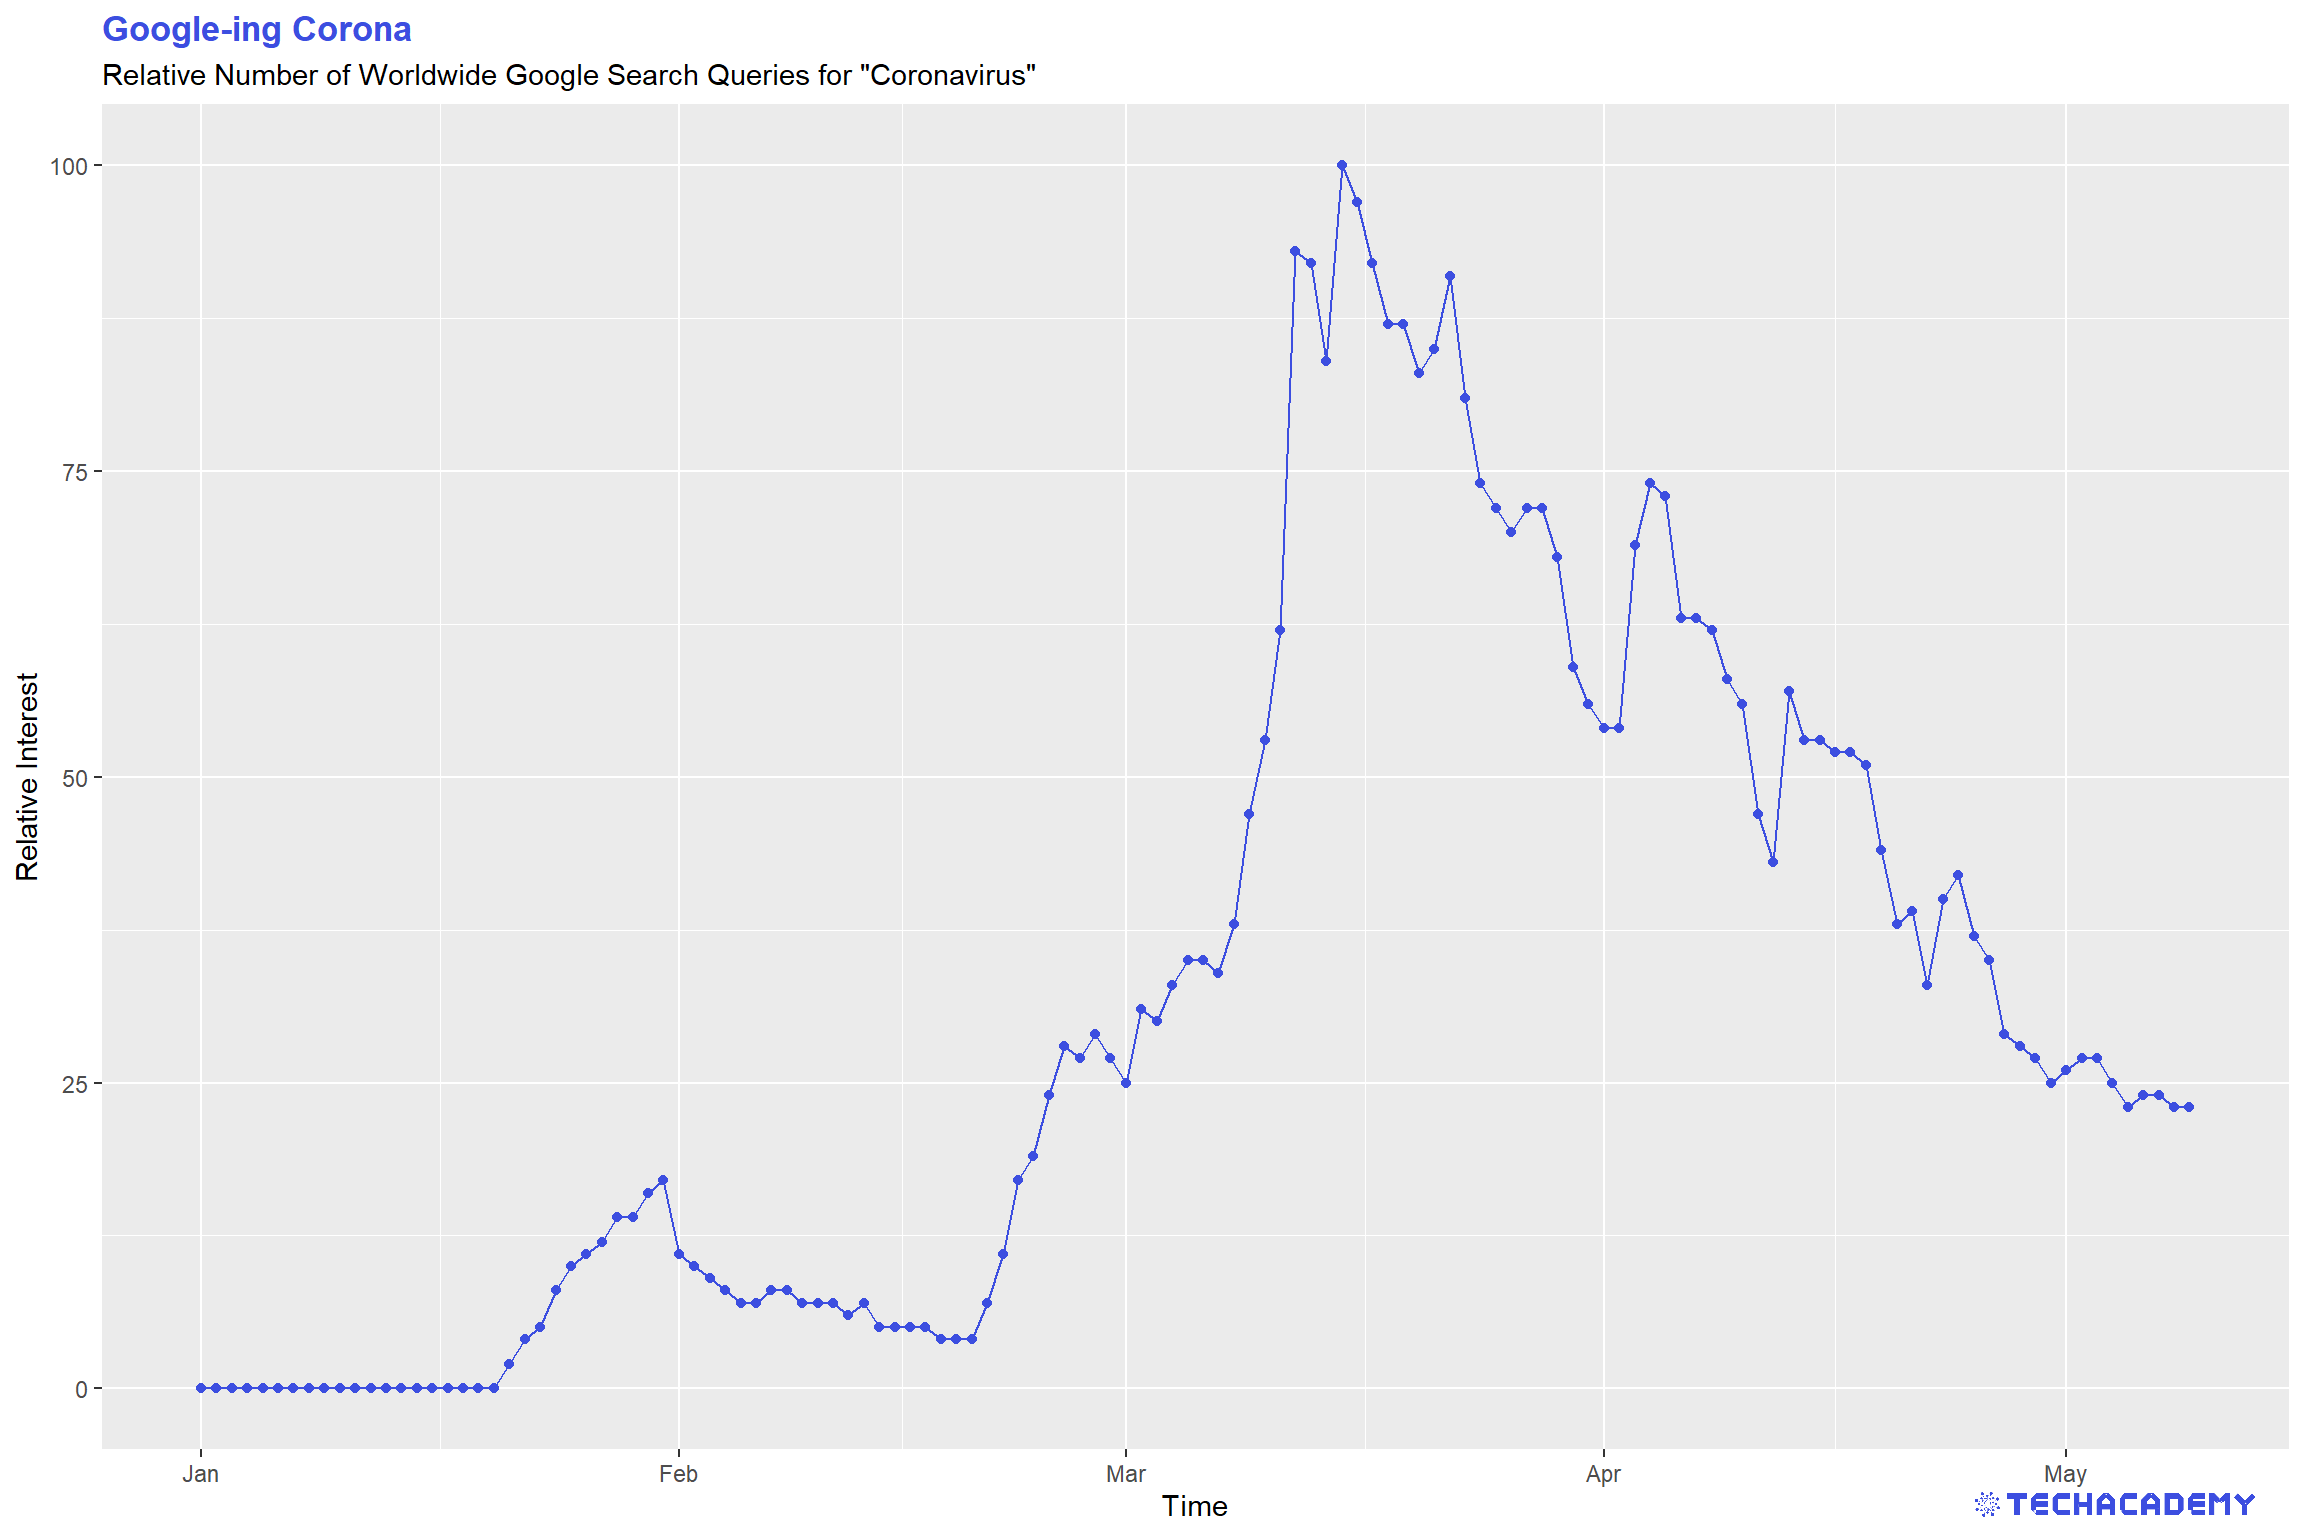
\includegraphics{output_files/figure-latex/unnamed-chunk-2-1.pdf}

Looking at the line plot, you can see a clear pattern with respect to different dates. Do you know what happened on the dates the spikes in searches occurred? If you have time you can play with the visualization and refine it, add labels and change colors, but that is not too important, so you can first have a look at the following steps and come back to this when you have completed the rest.

\begin{tips}r

\texttt{R} provides many different ways to import data. For starters, use the built-in \texttt{base} function \texttt{read.csv()} and define the path to the Google Trends file in the argument of the function. We have stored all data for your project in the folder \texttt{data}. Don't forget to use quotation marks \texttt{”...”} for the path -- you always need to use them when you specify \texttt{string}-variables in \texttt{R}. Also, you will need to adapt to the \texttt{R}-way of specifying paths. Defining a file path can either be done with \texttt{\textbackslash{}\textbackslash{}} or \texttt{/}, but not via a single backslash \texttt{\textbackslash{}} like in your explorer.

Use the \texttt{base} functions \texttt{str()} and \texttt{summary()} to print useful information on the data type and summary statistics for your \texttt{gtrends} data set.

Converting data types is relatively straightforward. Just use the useful functions in the format \texttt{as.\textless{}\textless{}insert\ data\ type\ here\textgreater{}\textgreater{}}. If you don't convert the \texttt{date} variable from a factor to a more useful data type, you will have problems plotting it.

For your first plot, use the simple \texttt{base} function \texttt{plot()} and define the two relevant input vectors for the time and the relative number of searches. While this function is great for very fast initial plots, you will need a more advanced graphics package later on. Do the same plot again with \texttt{ggplot2}. That gives you way more control and flexibility over plotting. Remember from your DataCamp courses that you first need to install a package once and then load it with the \texttt{library()} command at the beginning of your \texttt{R} session.

\end{tips}

\begin{tipsp}p

To import csv-files into your Jupyter notebook and to convert them into a pandas data frame use pandas' \texttt{.read\_csv()} method.
To read the data, you have to tell pandas the path to the files in the data folder from your current directory. To traverse upwards in the directory structure, you have to use two dots, so something like \texttt{../data/\textless{}here\ the\ rest\ of\ the\ path\textgreater{}} should work. For the first plot you need the Google trends data.
Afterwards use pandas' \texttt{.head()}, \texttt{.describe()}, and the \texttt{.info()} methods to explore the data: Are the dates actually stored as datetime objects? If not, you can change objects to datetime with \texttt{pd.to\_datetime(df.date,\ format=’\%Y-\%m-\%d’)}, where \texttt{df} stands for the data frame.
It would probably make sense to have the date-column set as index: You can do so by applying the \texttt{.set\_index(‘date’)} method to your data frame.
Now the only thing left to do is to plot your first graph!

\begin{Shaded}
\begin{Highlighting}[]
\NormalTok{plt.plot(df[‘hits’])}
\end{Highlighting}
\end{Shaded}

Make the plot visually more appealing by using additional pyplot methods and by passing additional arguments to those methods. For example:

\begin{itemize}
\tightlist
\item
  For the \texttt{.plot()} method you can use additional keyword arguments, like \texttt{color}, \texttt{marker}, \texttt{linewidth}, \texttt{linestyle}, and \texttt{markersize}.
\item
  Use the \texttt{.legend()} method to add a legend.
\item
  You can also add labels to your x- and y-axis by passing a string argument to the \texttt{.xlabel()} and \texttt{.ylabel()} methods.
\item
  You can rotate the ticks on the x-axis with \texttt{.plt.xticks(rotation=45)}.
\end{itemize}

Find a full list of methods in the \href{https://matplotlib.org/3.1.1/api/pyplot_summary.html}{official matplotlib documentation}.

\end{tipsp}

\hypertarget{visualize-stock-data}{%
\subsection{Visualize Stock Data}\label{visualize-stock-data}}

The coronavirus had an impact on many areas of our lives and our economy, the stock market being one of them. When visualizing the stock data, the impact becomes evident. Many firms suffered from the outbreak, others profited. Let's have a look!

As before, you first need to import the stock market dataset and name it accordingly. Once more, it makes sense to get an overview of the data to see what you are working with. Can you already see which variables need to be transformed?

Before visualizing the stock data, try to change the names of the stock symbols, so that people who are not familiar with them know which firm's stocks are being analyzed.

This time, we will not create a single line plot but several next to each other, which allows for a better comparison of the stock price development of different firms. The following plots are supposed to give you an orientation of what your result could look like:

You can often see vertical lines in the plots to highlight when an event happened that had a severe impact on a variable. Try to add that to the plots. Here is an idea of what it could look like:

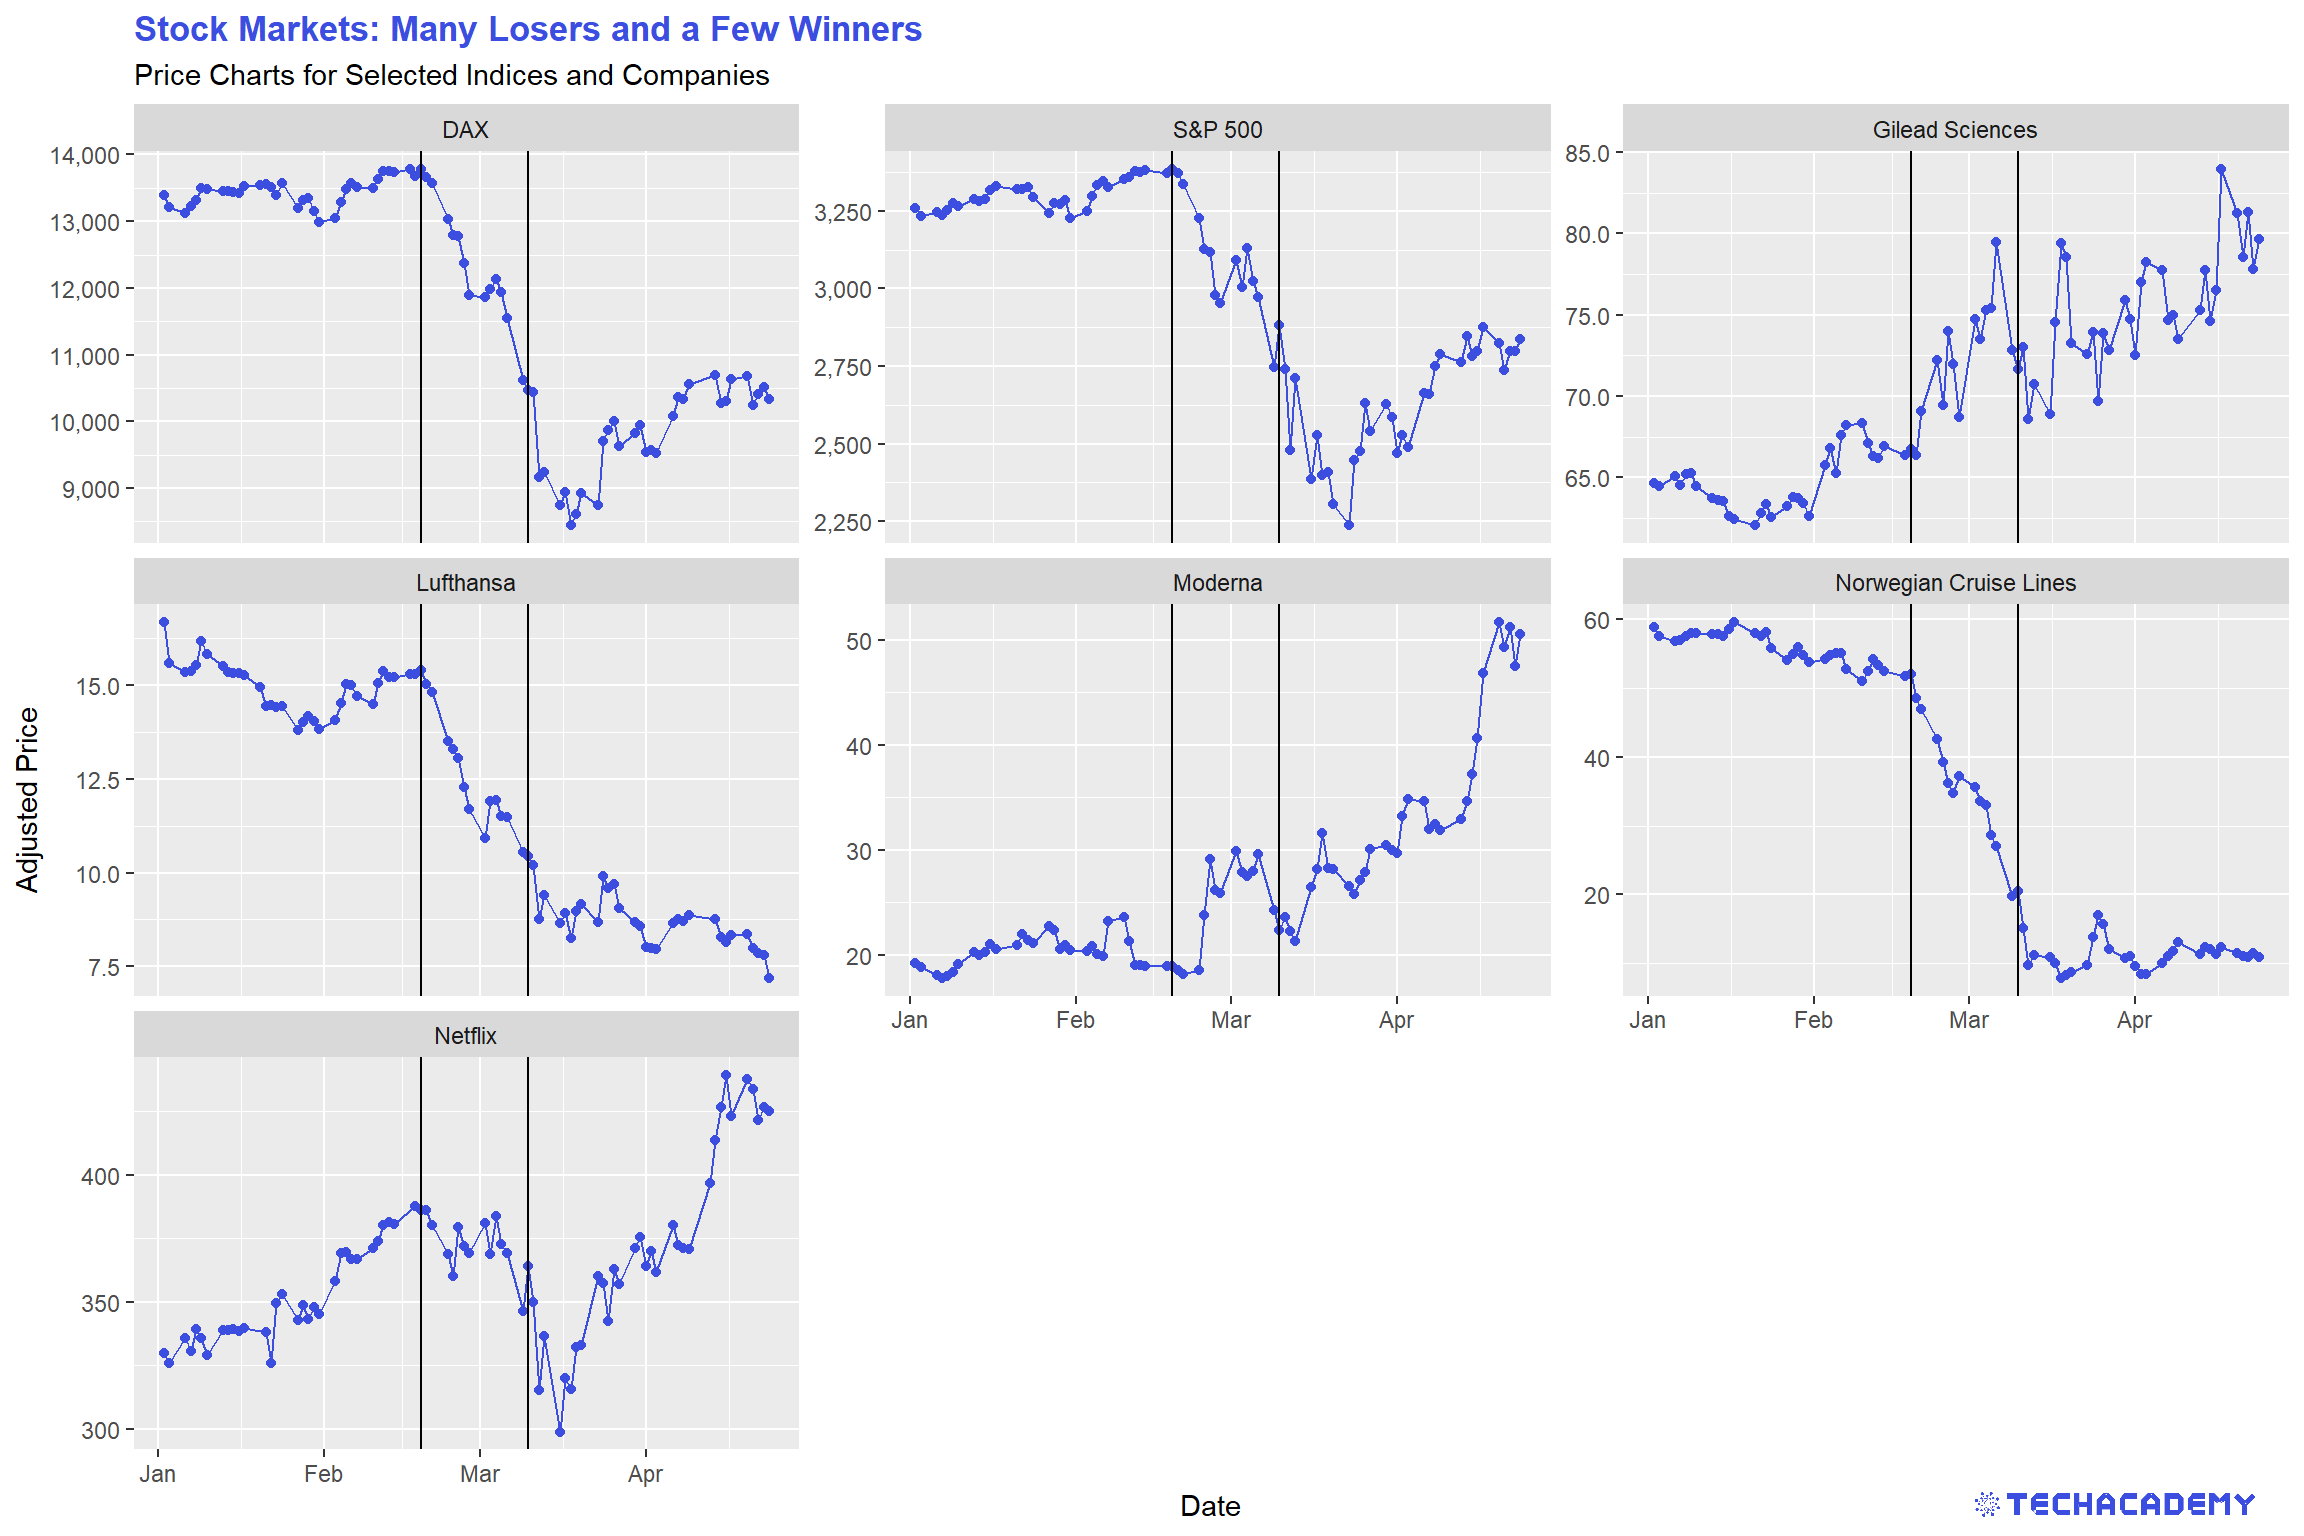
\includegraphics{output_files/figure-latex/unnamed-chunk-4-1.pdf}

After you visualized the data, think about what the data tells you and which key statements you can derive and communicate with your visualization. Take those ideas and put them into the title and subtitle of the graph. This practice leads the consumers of your visualizations directly to your key message. People looking at your graph for the first time will then more easily and faster spot the important takeaways from your plot.

\begin{tips}r

Use the package \texttt{ggplot2} and add \texttt{facet\_wrap()} after you specified the essential geom(s) to automatically create individual subplots.

Then look at how much more complex this task is in \texttt{Python} and be happy that you chose \texttt{R}.

To draw vertical lines to your plots, use another \texttt{geom} and simply add it to your \texttt{ggplot}.

You can label individual entries of a factor-type vector. That doesn't change the specific entries in the vector, but changes how the entries are displayed for example in plots. Use the function \texttt{levels()} to define the levels of the stock symbols.

\end{tips}

\begin{tipsp}p

Import the stock data as a data frame and explore the data, just as you've done with the Google Trends data. Notice that by using only the \texttt{.head()} method, one could think that the csv-file contains only data about one single stock -- this is not the case.

It would probably be easier to work with a data frame which only contains the columns we actually need, i.e.~\texttt{symbol}, \texttt{date}, and \texttt{close}. Also, it would probably be nicer to work with the data frame if the \texttt{date} column would be the index column, the values of the \texttt{symbol} column would represent the column names, and the \texttt{close} prices would be the data frame's values: Let's use pandas' \texttt{.pivot()} method to achieve both at once: \texttt{df.pivot(index=...,\ columns=...,\ values=...)}.

Check if the new index is formatted as a datetime object. If not, apply the same method as you did on the Google Trends data frame.
Now take a look at the whole data frame: Do you notice the \texttt{NaN}s? Try to find out why this is the case by searching it up online. However, if we would plot this data frame in a plot, we might end up with broken lines. One workaround to avoid this, could be to use the \texttt{.interpolate()} method on the data frame, which fills the \texttt{NaN} values using a linear method by default.

To create multiple plots in one figure you can use the example code below as a template. The code starts by creating a figure object, which is a container for plot elements. The function \texttt{plt.subplot(2,2,i)} adds a plot in the i-th window of the 2x2 grid inside the figure. Then, the data frame is filtered by the Netflix stock and the \texttt{plt.plot()} method is used to create the first plot.
Continue filling the next windows of the 2x2 grid with stock data from other companies.

\begin{Shaded}
\begin{Highlighting}[]
\NormalTok{fig }\OperatorTok{=}\NormalTok{ plt.figure(figsize}\OperatorTok{=}\NormalTok{(}\DecValTok{20}\NormalTok{,}\DecValTok{8}\NormalTok{))}
\NormalTok{plt.subplot(}\DecValTok{2}\NormalTok{,}\DecValTok{2}\NormalTok{,}\DecValTok{1}\NormalTok{)}
\NormalTok{data }\OperatorTok{=}\NormalTok{ stocks[stocks.symbol}\OperatorTok{==}\NormalTok{ symbols[‘NFLX’]][}\StringTok{\textquotesingle{}close\textquotesingle{}}\NormalTok{]}
\NormalTok{plt.plot(data)}
\end{Highlighting}
\end{Shaded}

You can add a vertical line to point out a date where stock prices started to become very volatile with \texttt{plt.axvline(x=pd.Timestamp(\textquotesingle{}YYYY-MM-DD\textquotesingle{}),\ ymin=0,\ ymax=1)}, whereby x is the coordinate for the x axis, ymin is the bottom and ymax the top of the line.
You used pretty much the same code four times in a row, in such a case it is often good to use a for-loop of the form:

\begin{Shaded}
\begin{Highlighting}[]
\ControlFlowTok{for}\NormalTok{ i }\KeywordTok{in} \BuiltInTok{range}\NormalTok{(}\DecValTok{4}\NormalTok{)}
    \CommentTok{\# your code here}
\end{Highlighting}
\end{Shaded}

Can you find a way to reduce your code using a for-loop? Try to address the changing parts of your code with the index i in the for-loop.

Afterwards you can try to make your plot look nicer.
Use \texttt{fig.suptitle()} to add a title.
If you feel like needing to adjust spaces between the plots, you can use the \texttt{plt.subplots\_adjust()} to do so.
Try using \texttt{fig.autofmt\_xdate()} to format the date tick labels. If you need help with these functions, try to find out what they do and how to use them in the \href{https://matplotlib.org/3.2.1/contents.html}{matplotlib documentation}.

\end{tipsp}

\hypertarget{visualize-covid-19-infection-data}{%
\subsection{Visualize Covid-19 Infection Data}\label{visualize-covid-19-infection-data}}

\hypertarget{worldwide-development-of-confirmed-cases}{%
\subsubsection{Worldwide Development of Confirmed Cases}\label{worldwide-development-of-confirmed-cases}}

Over the last couple of months you heard new numbers about the coronavirus every day, so it is time to bring some clarity into the development of the virus in different countries over time. So now that we had a first look at certain data sets with a connection to the coronavirus, it is time to look at the coronavirus data itself.

The first data set that you are going to import contains data about the number of confirmed cases all over the world. Name it accordingly and once again, have a look at its structure.

As you can see, we have missing values in the confirmed variable. Your task will be to replace those with the value 0. We can do this because we can assume that if there is a missing value it is most likely that there has not been a confirmed case yet.

Once again it makes sense to create a simple line plot to take a look at the number of confirmed cases over time. In the first step, we will have a look at the worldwide development. For that you will have to transform the data. At this point, our data set has a separate number of confirmed cases for each country per day. In the end, our transformed data set should summarize this so that we only have one number per day that represents the aggregate number of confirmed cases worldwide.

This is what your plot could look like:
You can see that the line plot has a small kink around February 10th. Restict the y-axis if you don't see it on first glance to the interval \(y =[0,100.000]\). What happened at that point in time that had such a great impact on the number of confirmed cases?

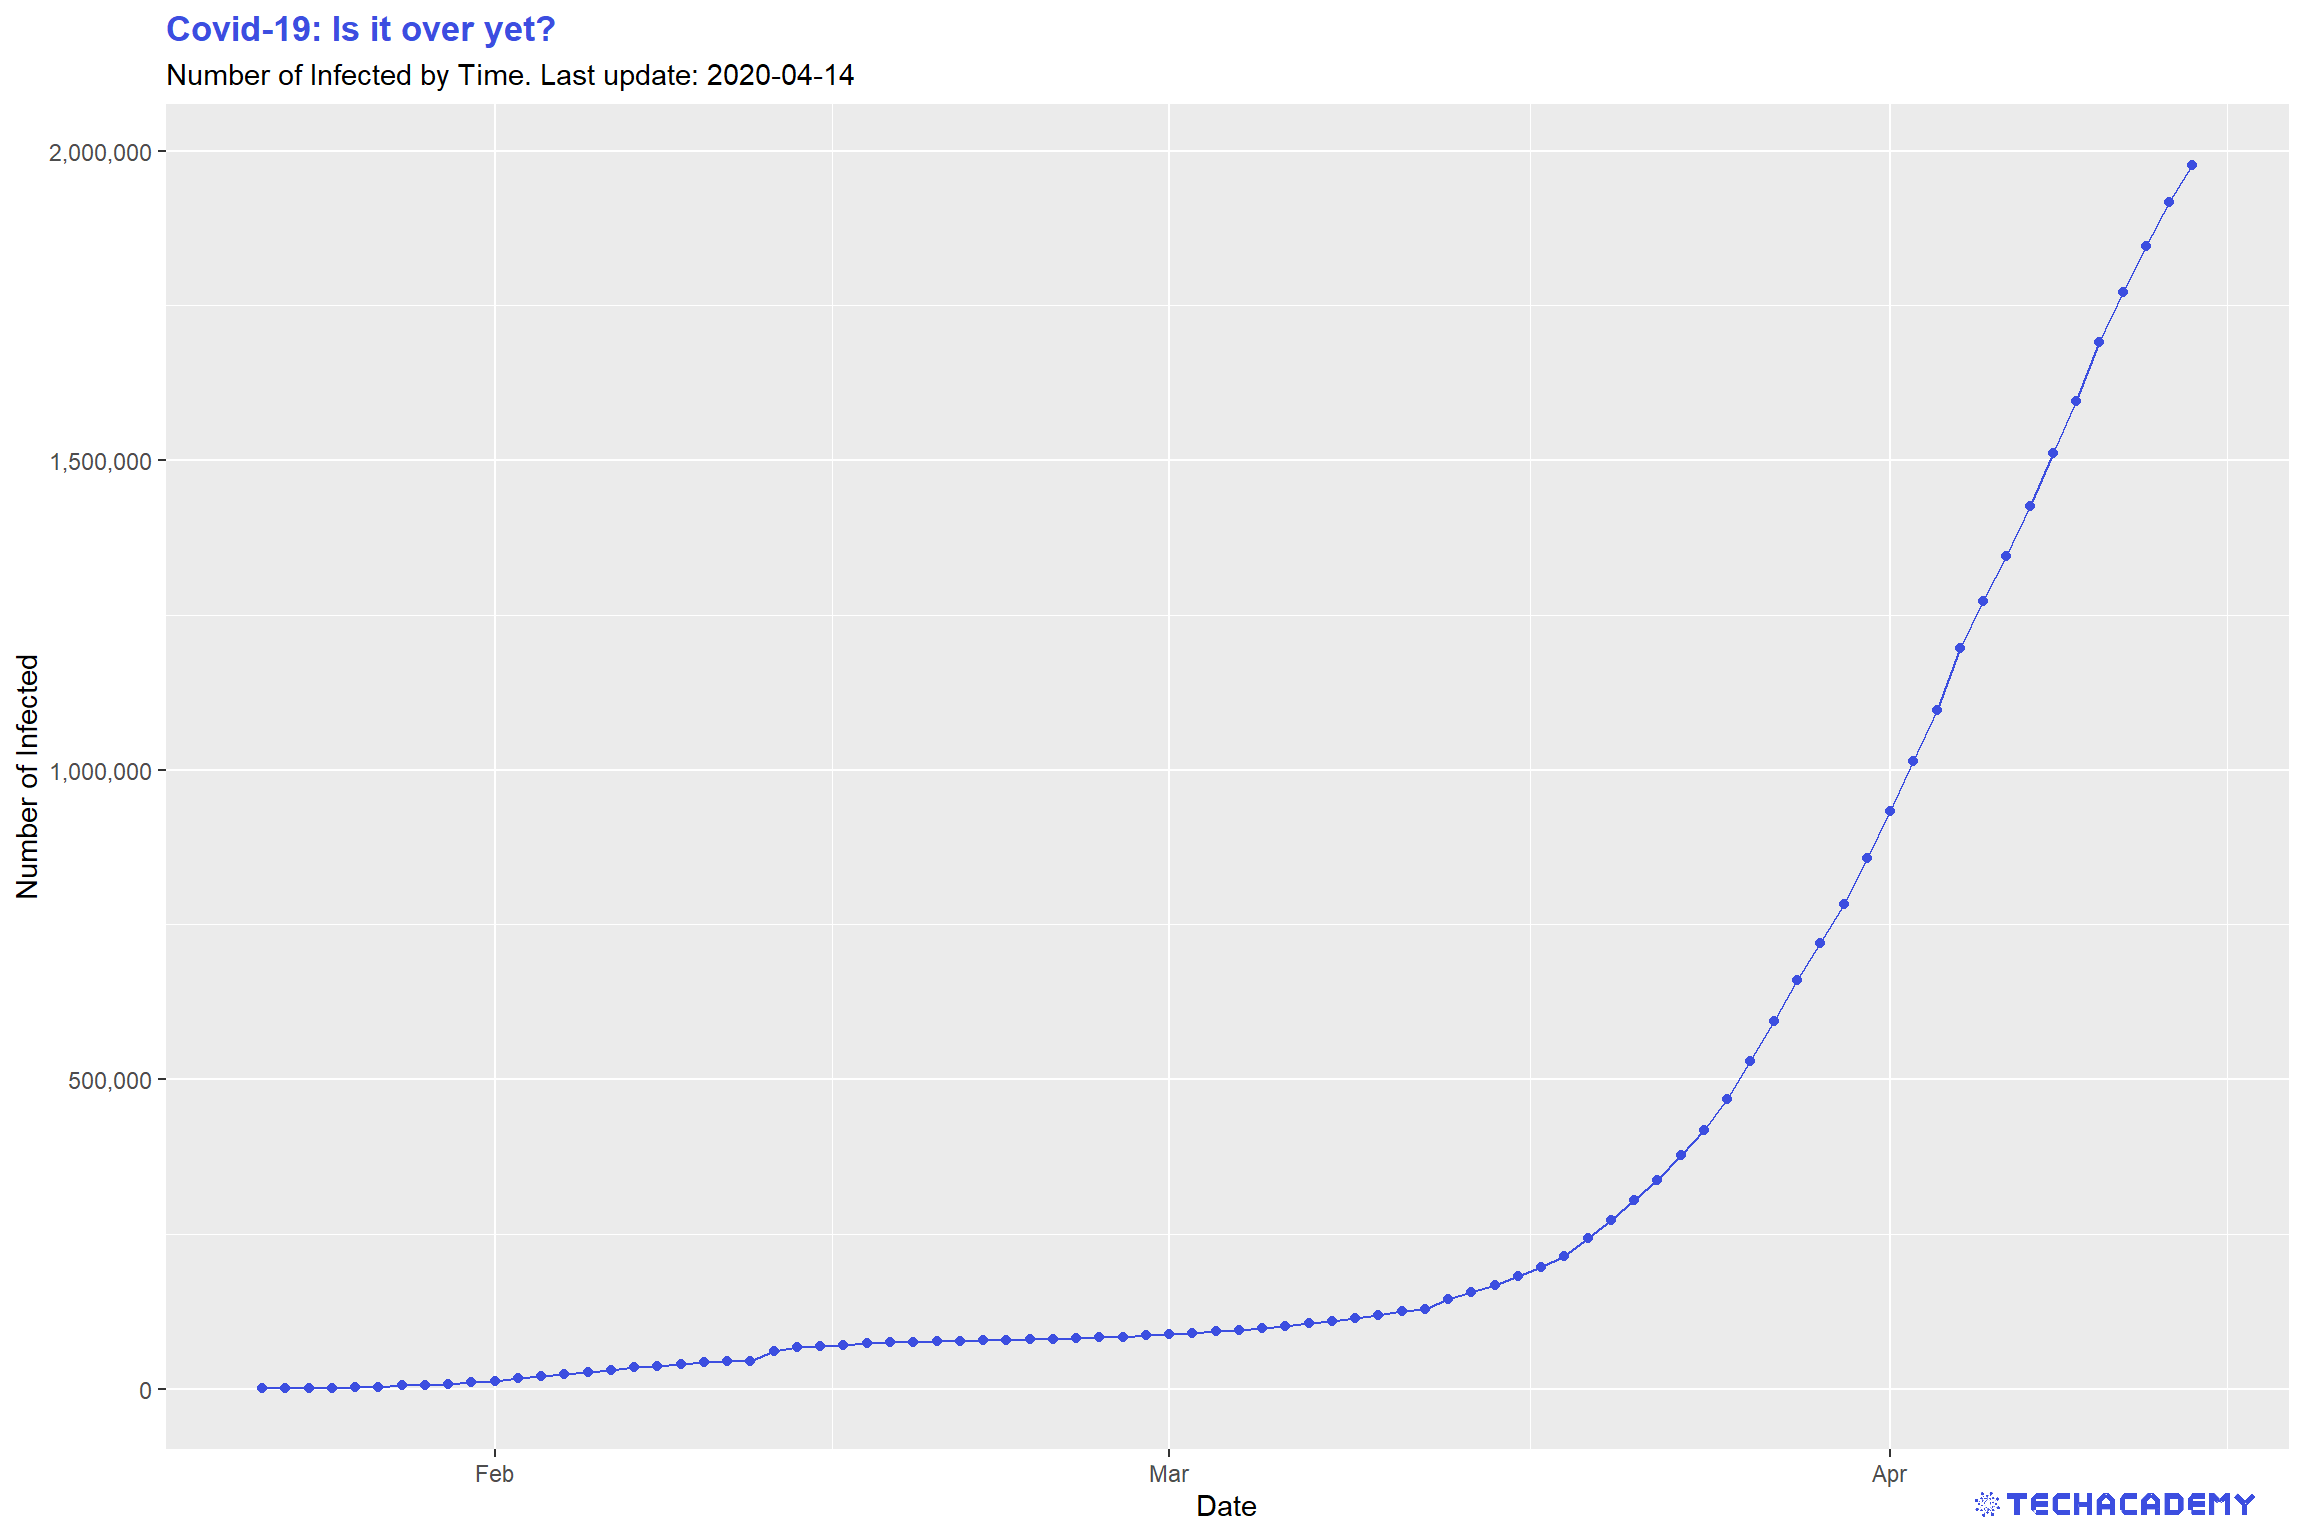
\includegraphics{output_files/figure-latex/unnamed-chunk-7-1.pdf}

\begin{tips}r

Import the new panel data set \texttt{confirmed.csv} and analyze its structure
like you did in the previous exercise. Are you noticing the \texttt{NA} entries in the variable \texttt{confirmed}? Replace those missing values with \texttt{0}. There are several ways to do that, one is using \texttt{ifelse()}. After you replaced the missing values, check if you were successful by summing up all entries in the logical vector generated by \texttt{is.na()}. If this sum is zero, you have replaced all \texttt{NA} values. This works because \texttt{R} treats the logical values \texttt{TRUE} and \texttt{FALSE} as \texttt{1} and \texttt{0}.

Also, \texttt{read.csv()} by default imports dates as factors. Transform the column \texttt{time} to the appropriate \texttt{date} variable type.

You've probably already heard about the \texttt{tidyverse} -- a highly influential and very useful set of packages that all follow a common philosophy. Even if it might be tough to get used to the tidy way of thinking, you will love it once you have understood it.

You can use the \texttt{dplyr} package to summarize \texttt{confirmed} by \texttt{time}. Remember the pipe-operator \texttt{\%\textgreater{}\%} from the DataCamp course \href{https://www.datacamp.com/courses/data-manipulation-with-dplyr-in-r}{Data Manipulation with dplyr in R}? This operator will come in handy to build longer data transformation pipelines. Use a combination of the \texttt{dplyr} functions that group and summarize data. In case you don't remember their names and arguments, familiarize yourself with the \texttt{dplyr} documentation by typing \texttt{?dplyr} into your console or by googling the problem. In general, \texttt{?} leads you to the documentation of packages or functions in \texttt{R}.

Use \texttt{ggplot2} again to visualize your newly generated time series. Don't forget to provide meaningful labels for your title, subtitle and axes.

\end{tips}

\begin{tipsp}p

Import the \texttt{confirmed.csv} data as a new data frame and fill the empty spaces (\texttt{NaN}) using \texttt{.fillna(0)}. Afterwards you can use \texttt{df.isna()} to check if there are no missing values in the data frame. This will return True (corresponds to 1) and False (corresponds to 0) if there is a missing value or not. If you \texttt{sum()} over this data frame, you get the amount of missing values which should be zero now.

Since we are not interested in every single country's number of confirmed cases yet, the idea is to group all dates together by summing up the numbers of confirmed cases for each day. You can use pandas' \texttt{groupby()} function, which itself returns no result -- you also have to apply an aggregation function like \texttt{groupby(by=’time’).max()}, \texttt{groupby(by=’time’).mean()} or \texttt{groupby(by=’time’).sum()}. For this task you can use the latter.
The time column should now be set as index -- make sure that its values are formatted as datetime objects.
Finally, you can create the graph by passing the right column of the data frame to the \texttt{plot()} method of the matplotlib library.

\end{tipsp}

\hypertarget{stacked-area-plot-by-country}{%
\subsubsection{Stacked Area Plot by Country}\label{stacked-area-plot-by-country}}

You have gained some experience in creating simple line plots so let's take it a step further and create a stacked area plot for the countries with the highest number of confirmed cases. The idea behind this is that you add up individual time series and color the area in between by country. This is a little tricky but with patience you will get there. The first step will be to select the countries with the highest number of confirmed cases on the most recent date of the data set. The result should look similar to this:

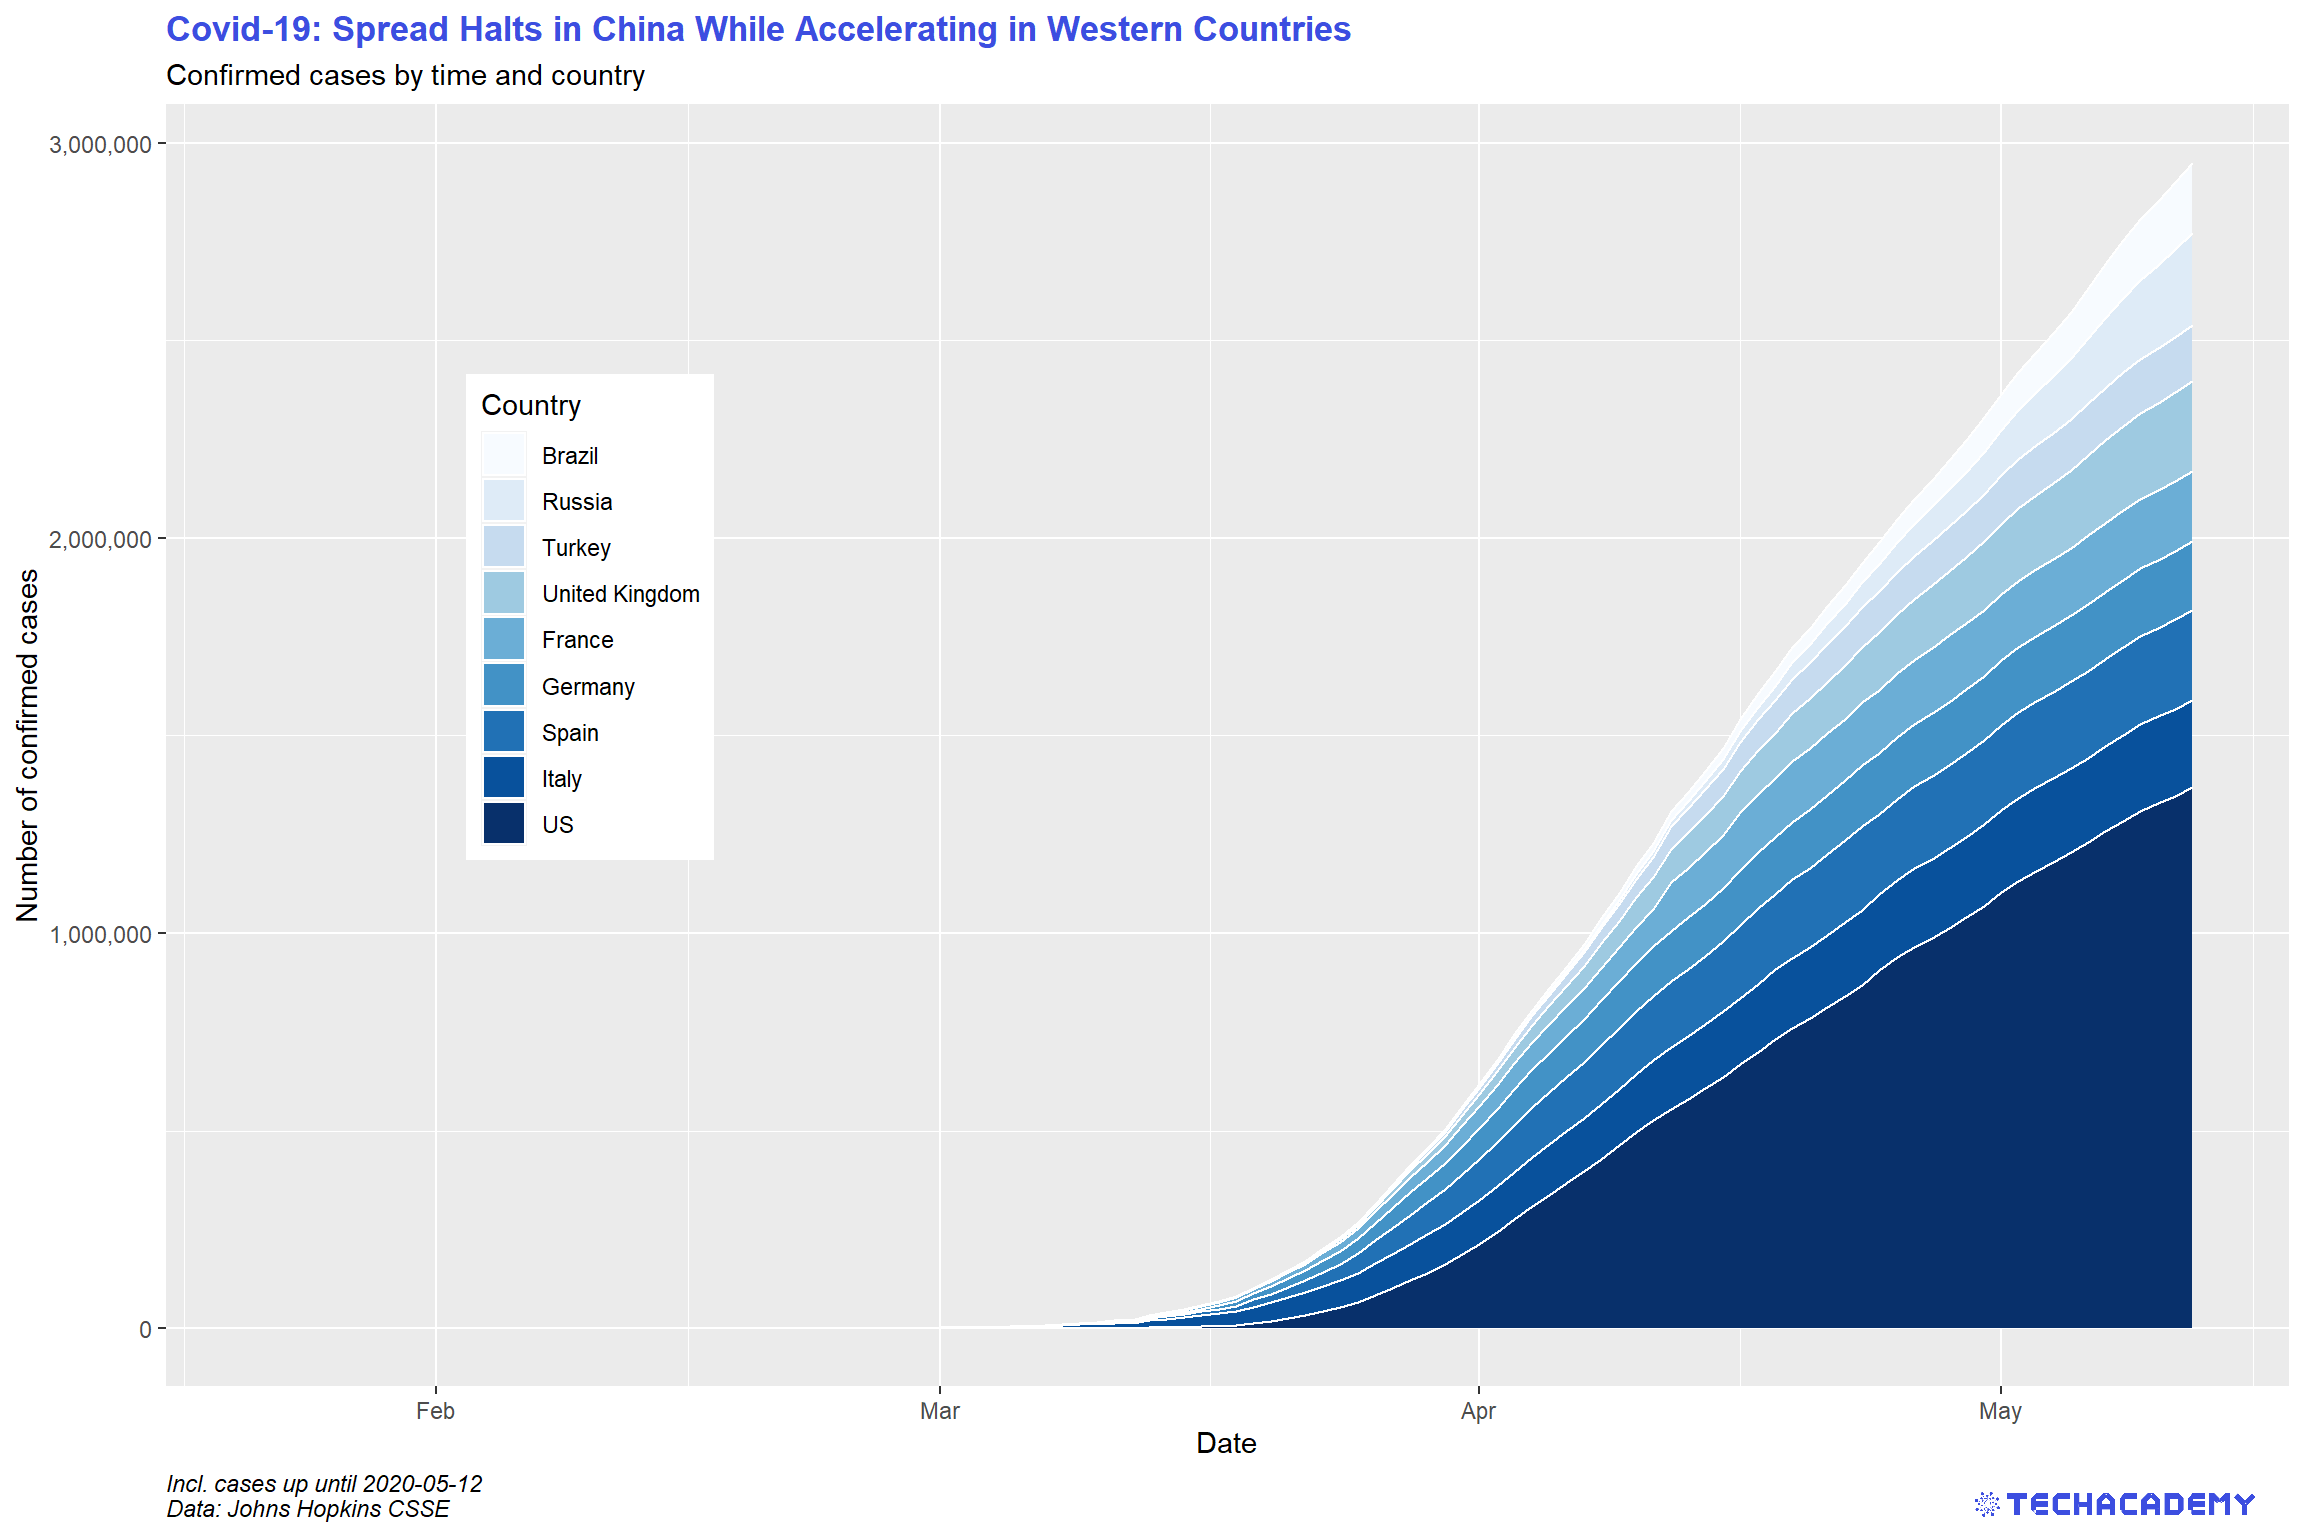
\includegraphics{output_files/figure-latex/unnamed-chunk-8-1.pdf}

\begin{tips}r

First, extract the names of the nine countries that are most affected on the most recent date. Use \texttt{filter()} to only keep the most recent date. You should use \texttt{arrange()} to order the data frame in descending order by \texttt{confirmed}. Then extract the top nine entries and select the column \texttt{country}. Save this vector as \texttt{top\_countries} for later use.

Now prepare the data set for plotting. Filter it such that only data for \texttt{top\_countries} remains. You might want to use the \texttt{\%in\%} operator for that task.

To draw the plot, use \texttt{ggplot2} and add the geom that generates an area plot.

The countries in the plot are not ordered in an ideal way for this visualization -- countries are sorted alphabetically. Remember \texttt{levels()} that define the ordering of \texttt{factor} variables? Order those by \texttt{confirmed} cases, such that the most affected country comes last.

\end{tips}

\begin{tipsp}p

First you need to know which are the 9 countries with the most confirmed cases. Use the \texttt{groupby()} function with the appropriate aggregation function.

Afterwards you can sort the returned data frame with the \texttt{df.sort\_values()} function and use index slicing to get only the first 9 entries of the data frame. Then store it under the variable name \texttt{top\_countries}.

Now we know which countries should be visualized in the plot. For each of these countries we need the amount of confirmed cases over time. To get the confirmed cases for one country, we filter the whole data frame by this country and afterwards group the filtered data frame by time.

Because we have to repeat the same procedure with each of the 9 countries, it is a good idea to use a for-loop and iterate over the list of countries stored in \texttt{top\_countries}.

\begin{Shaded}
\begin{Highlighting}[]
\CommentTok{\# store data in list}
\NormalTok{confirmed\_list }\OperatorTok{=}\NormalTok{ []}
 
\CommentTok{\# for{-}loop over the countries}
\ControlFlowTok{for}\NormalTok{ country }\KeywordTok{in}\NormalTok{ top\_countries:}
\NormalTok{    confirmed\_list.append(}\CommentTok{\#your code to filter confirmed cases by country)}
\end{Highlighting}
\end{Shaded}

In each iteration of the for-loop, append only the values of confirmed cases to a list which you instantiate before the for-loop. At the end of the for-loop you should have a list of pandas series (data frame with just one column) , each containing only the amount of confirmed cases per country over time. To get only values of a pandas series, you can use \texttt{df{[}\textless{}column\_name\textgreater{}{]}.values}.

This list contains the amount of confirmed cases, but not the dates. The dates are the same for each country, so we just need to get a pandas series of one of the filtered countries, select the \texttt{time} column and store it under the variable \texttt{dates}.

To get the stacked area chart, you can use the matplotlib function \texttt{plt.stackplot(x,y,labels)}. For the y values you can just pass the list of data frames which we created before and the x values should be the list of dates. The labels are the corresponding names of the countries.

\end{tipsp}

\hypertarget{all-curves-in-one-plot}{%
\subsubsection{All Curves in One Plot}\label{all-curves-in-one-plot}}

Having had a closer look at the confirmed cases, we can go ahead and get more into detail by adding data of dead and recovered patients. But we don't want to keep the three data sets separate, so your next task is to merge the three data sets before we analyze the numbers more thoroughly. You can have a first glimpse at the data and look at the structure. You can see that all three data sets share the same structure, and identical observations share the same ID. This makes it easy because it allows you to merge them by ID.

Similar to your first data set, the merged data frame has missing values. Replace them once again with the value 0.

When talking about the coronavirus many people are only mentioning the total number of confirmed cases. But it makes sense to keep track of the currently infected patients and not only the total infected. This way it is easier to see whether the virus is actually receding or still on the rise. This means we want to have a look at the number of confirmed cases that are still infected and not dead or healed already. For this you can subtract the number of deaths and recovered cases from the number of confirmed cases and create a new variable that you can call \texttt{netinfected}. Visualize the development of confirmed cases, deaths, netinfected, and recovered in an area plot for the top 9 countries.

A quick remark on the underlying data for \texttt{recovered} and thereby also \texttt{netfinfected}: At first, Johns Hopkins University (JHU) provided the variable \texttt{recovered}. Over time, gathering reliable data on the number of healed patients grew increasingly difficult.
German hospitals for example have no legal obligation to report when a patient recovered.
That's why JHU stopped providing this data. As a quick work-around, we assume that two weeks after patients were infected they count as recovered if they did not die. This is a rough estimate and will not always be true, but sometimes you have to make some reasonable assumptions to work with real-world data.

If everything went well your result will look similar to this:

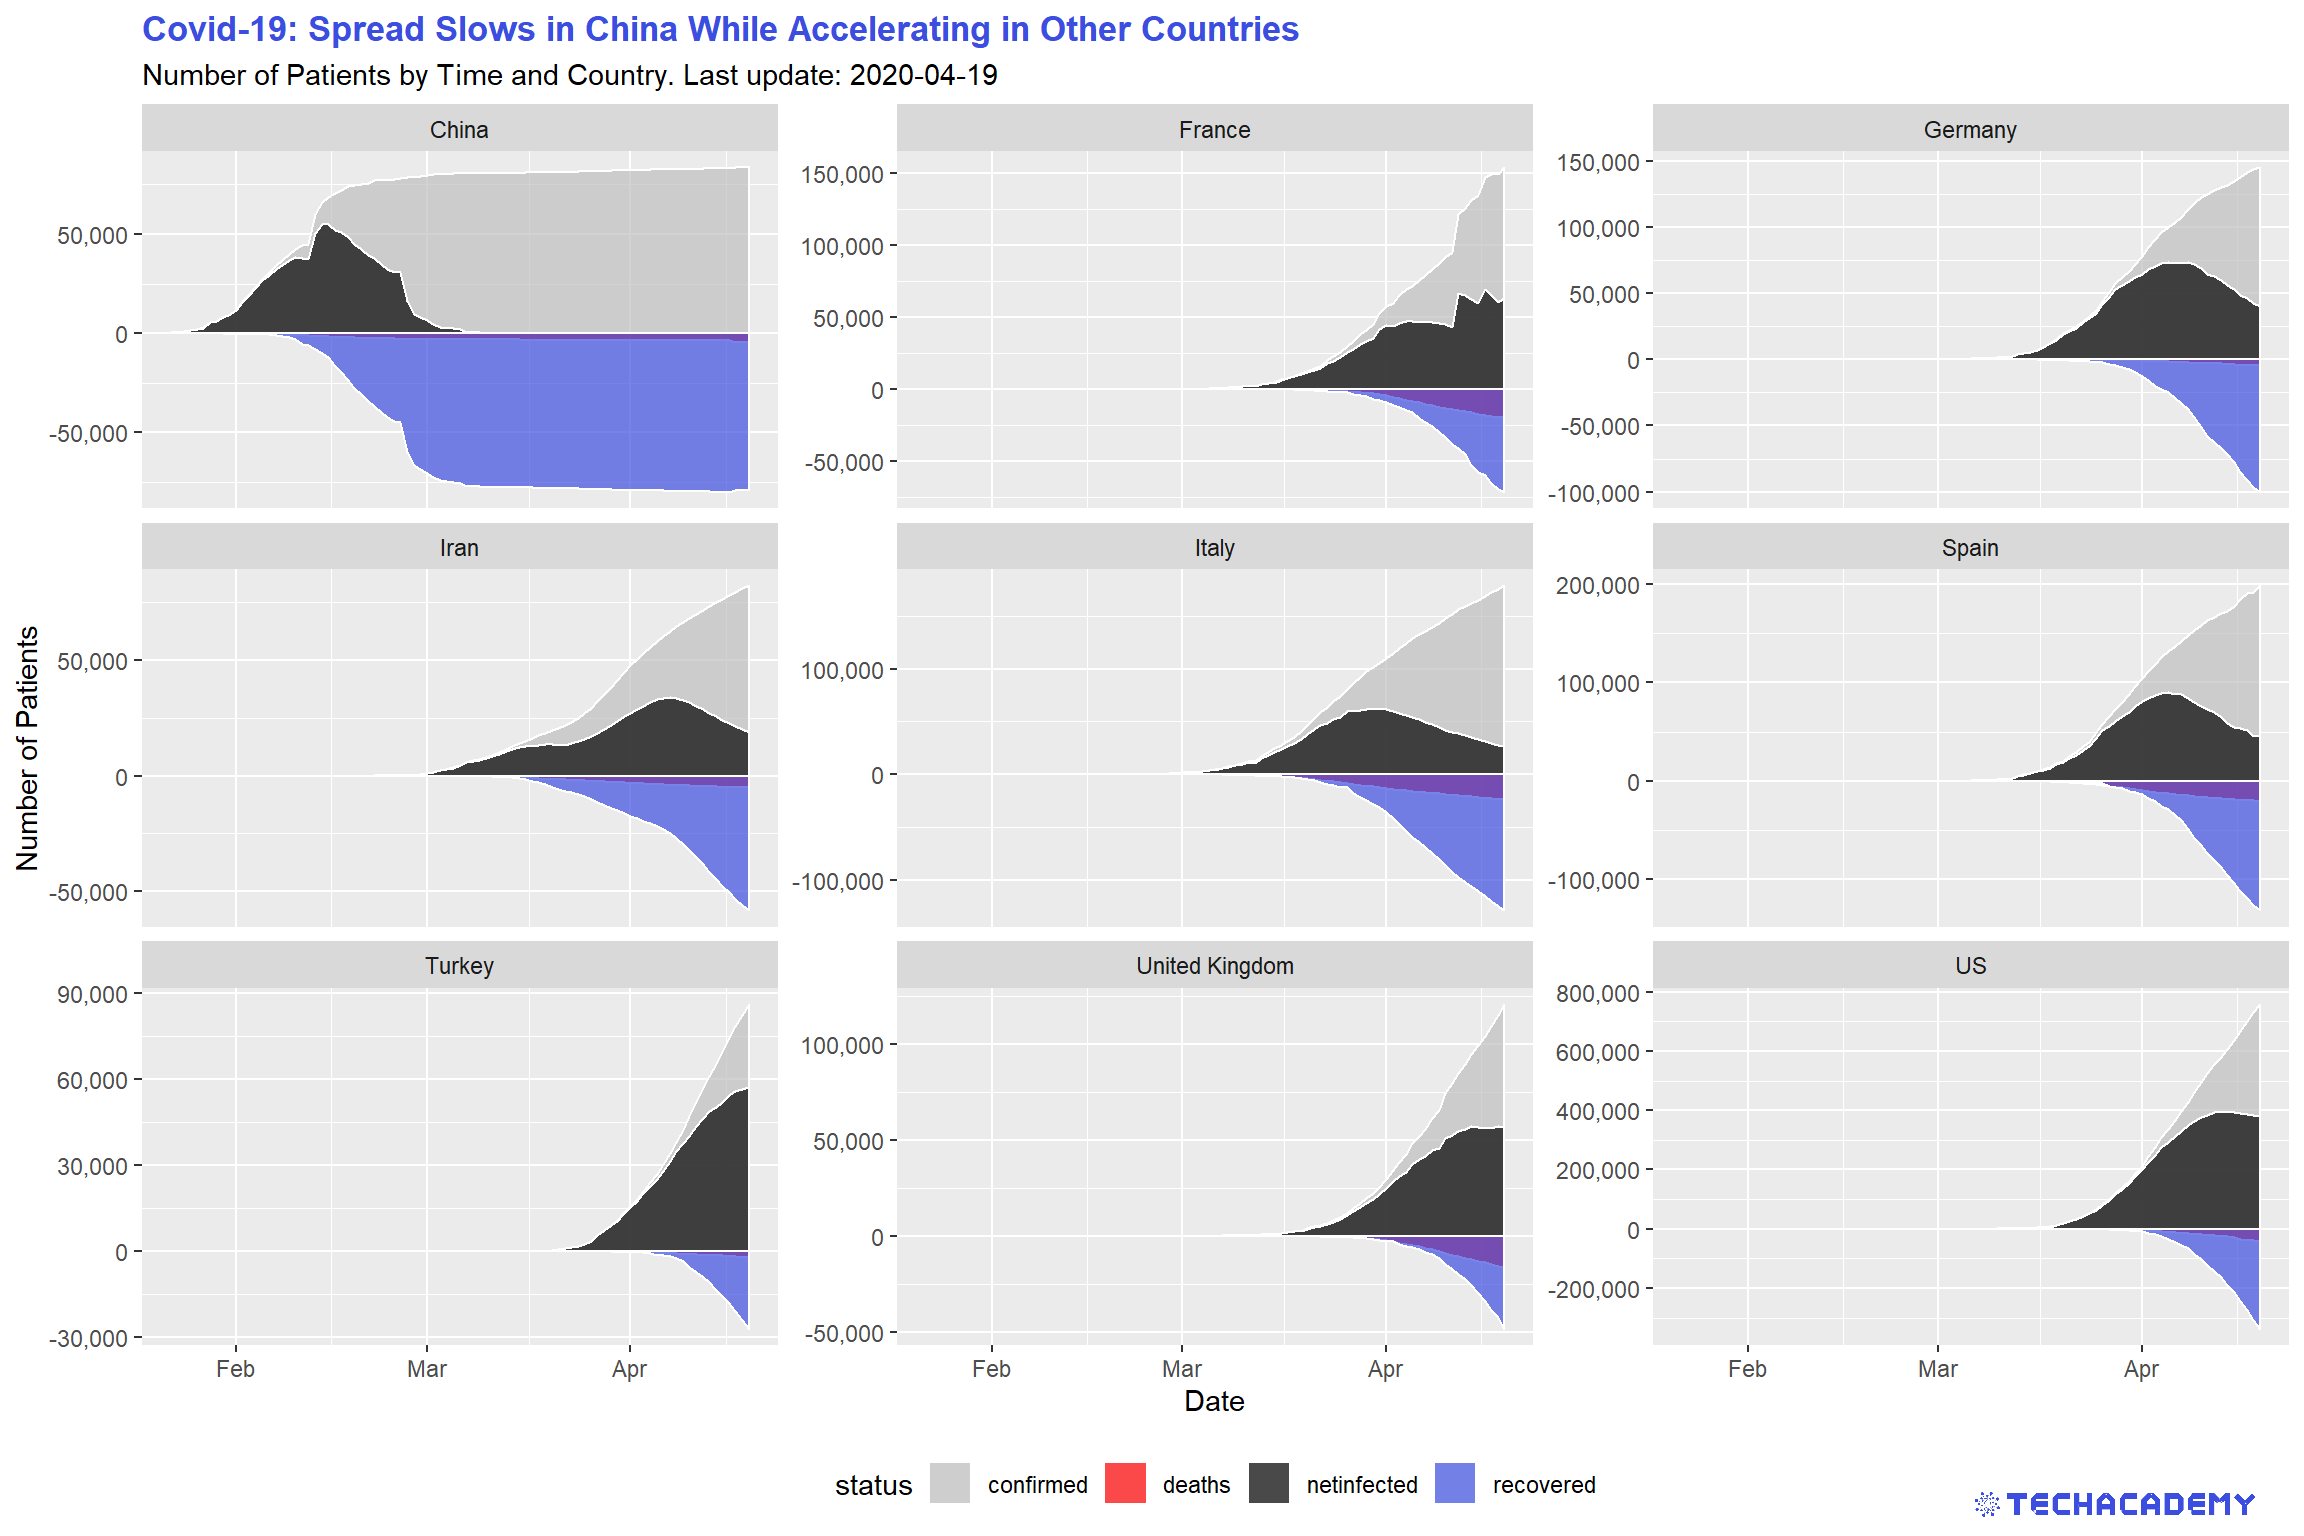
\includegraphics{output_files/figure-latex/unnamed-chunk-11-1.pdf}

\begin{tips}r

Import the data sets \texttt{deaths.csv} and \texttt{recovered.csv} and check out their format and structure. Notice that similarly to \texttt{confirmed.csv}, they also include the column \texttt{id}, which uniquely identifies a single date for one country across those data sets.

Now merge the three data frames by \texttt{id} into \texttt{df\_merged}, which should include all three quantities \texttt{confirmed}, \texttt{deaths}, and \texttt{recovered}. You can either use the \texttt{base} function \texttt{merge()} or the more powerful \texttt{...\_join()} from the \texttt{dplyr} package. \texttt{...} stands for either \texttt{left}, \texttt{right}, \texttt{inner}, or \texttt{full}. Those adjectives define which columns to keep after merging. The \texttt{dplyr} \href{https://rstudio.com/wp-content/uploads/2015/02/data-wrangling-cheatsheet.pdf}{cheat sheet} provides a more detailed explanation on those tools.

After you merged the data frames, again replace the \texttt{NA} values with 0.
Now create the new variable \texttt{netinfected}. Use \texttt{\$} to specify the new variable and simply define it as the appropriate subtraction involving the three variables \texttt{confirmed}, \texttt{deaths}, and \texttt{recovered}.

After once again filtering the \texttt{top\_countries} from the full data set, we want to transform the data frame from a \emph{wide} format into a \emph{long} format. You have probably heard of \texttt{gather()} and \texttt{spread()} from the \texttt{tidyr} package in your courses. Those functions work well for this task, but there is an enhanced set of functions from the same package that just got released and work even more intuitively. Load \texttt{library(tidyr)} and familiarize yourself with the new functions \texttt{pivot\_longer()} and \texttt{pivot\_wider()}. Use one of them to accomplish the task. Use the structure below.

\begin{Shaded}
\begin{Highlighting}[]
\NormalTok{df\_merged }\OperatorTok{\%\textgreater{}\%}\StringTok{ }
\CommentTok{\# filter here}
\CommentTok{\# mutate here (optional)}
\StringTok{  }\KeywordTok{pivot\_...}\NormalTok{(}\OperatorTok{\textless{}}\ErrorTok{\textless{}}\NormalTok{first var to pivot}\OperatorTok{\textgreater{}}\ErrorTok{\textgreater{}:\textless{}\textless{}}\NormalTok{last var to pivot}\OperatorTok{\textgreater{}}\ErrorTok{\textgreater{}}\NormalTok{,}
            \DataTypeTok{names\_to =} \StringTok{"..."}\NormalTok{,}
            \DataTypeTok{values\_to =} \StringTok{"..."}\NormalTok{) }\OperatorTok{\%\textgreater{}\%}
\KeywordTok{ggplot}\NormalTok{() }\OperatorTok{+}
\NormalTok{...}
\end{Highlighting}
\end{Shaded}

Your first attempts might look totally weird. Play around with \texttt{ggplot2} by varying the type of plot (e.g.~line or area). You can visually separate the individual columns by assigning the variable \texttt{status} to the arguments \texttt{color\ =} and \texttt{linetype\ =} within the aesthetics of \texttt{geom\_line(aes(...))}.

Another enhancement of your visualization is to plot \texttt{recovered} and \texttt{deaths} on the negative part of the y-axis. This avoids overplotting and enables a better communication of the data. In the previous code chunk above is a predefined space to do just that transformation. Use \texttt{mutate()} to replace the values of the two variables with its negative ones.

\end{tips}

\begin{tipsp}p

First, we need to merge the data frames \texttt{confirmed}, \texttt{deaths} and \texttt{recovered} -- which means we want to form one big data frame containing the information of the three individual data frames. They share the same column \texttt{id} and can be merged over this value. You can merge two data frames with the pandas merge function: \texttt{merged\_df\ =\ pd.merge(df1,\ df2,\ on=’id’)}. Now you still need to merge the third data frame.

After the three data frames are merged, we have to fill up \texttt{NaN}s (missing values) with the pandas \texttt{df.fillna(0)} function.

Now we want to compute the amount of \texttt{netinfected} people, which can be computed by \texttt{netinfected\ =\ confirmed\ –\ recovered\ –\ deaths}. Create a new column in the data frame and compute this value for each row.

We want to plot four time series per country. Therefore, we filter the complete data frame after the corresponding countries and use, similar to the exercise before, the \texttt{df.groupby()} function and group now by \texttt{time}. Again we have to use the right aggregation function on the \texttt{groupby()} function. But this time we need -- besides the \texttt{confirmed} column -- also the \texttt{deaths}, \texttt{recovered} and \texttt{netinfected} columns. You could use a simple line plot with \texttt{plt.plot()} or the function \texttt{plt.fill\_between(x,y)} to get a plot which looks similar to the given example.

It is a bit tricky to get several plots into one figure, therefore we provide again an example code.

\begin{Shaded}
\begin{Highlighting}[]
\ControlFlowTok{for}\NormalTok{ i }\KeywordTok{in}\NormalTok{ [}\DecValTok{1}\NormalTok{,}\DecValTok{2}\NormalTok{,}\DecValTok{3}\NormalTok{,}\DecValTok{4}\NormalTok{,}\DecValTok{5}\NormalTok{,}\DecValTok{6}\NormalTok{]:}
\NormalTok{    plt.subplot(}\DecValTok{2}\NormalTok{,}\DecValTok{3}\NormalTok{,i)}
\NormalTok{    plt.fill\_between(x\_data, y\_data)}
\end{Highlighting}
\end{Shaded}

Fill the \texttt{plt.fill\_between()} or \texttt{plt.plot()} function in each iteration of the for-loop with data of another country and the graphs will be plotted in the corresponding windows of the plot-grid.
When you run your code and you can see a grid of plots, each showing four time series of different countries, you can be proud of you. You mastered an advanced concept of the matplotlib library -- which can be frustrating from time to time.

Now you can beautify the plot a bit. Add the name of the country as title to each plot (\texttt{plt.title(‘Taka-Tuka-Land’)}). The plots for \texttt{deaths} and \texttt{recovered} contribute negatively to \texttt{netinfected} and should be plotted as negative values as shown in the example plot. Furthermore, the x-ticks should show the date, but they are not readable at the moment.

Try to rotate the ticks and plot only every \(10^{th}\) date. To plot only every \(n^{th}\) tick is a bit challenging and we need help! We google something like \texttt{python\ matplotlib\ only\ nth\ tick}. Most of the time this will lead to the website Stackoverflow where somebody had the same problem as you and got help from other programmers. Look into the answers of \href{https://stackoverflow.com/questions/12608788/changing-the-tick-frequency-on-x-or-y-axis-in-matplotlib/31997618}{this Stackoverflow post}. Several users proposed possible solutions. Can you find one which works for you? And don't be afraid if you don't understand some parts of their code, try-and-error is a good way to learn and find solutions.

\end{tipsp}

\hypertarget{barplot-by-country}{%
\subsubsection{Barplot by Country}\label{barplot-by-country}}

Although this is a great way of visualizing the development of the virus outbreak, some characteristics are hard to make out in this kind of visualization. Hence, it makes sense to take the same measures and create a bar plot with them. This should look like this:

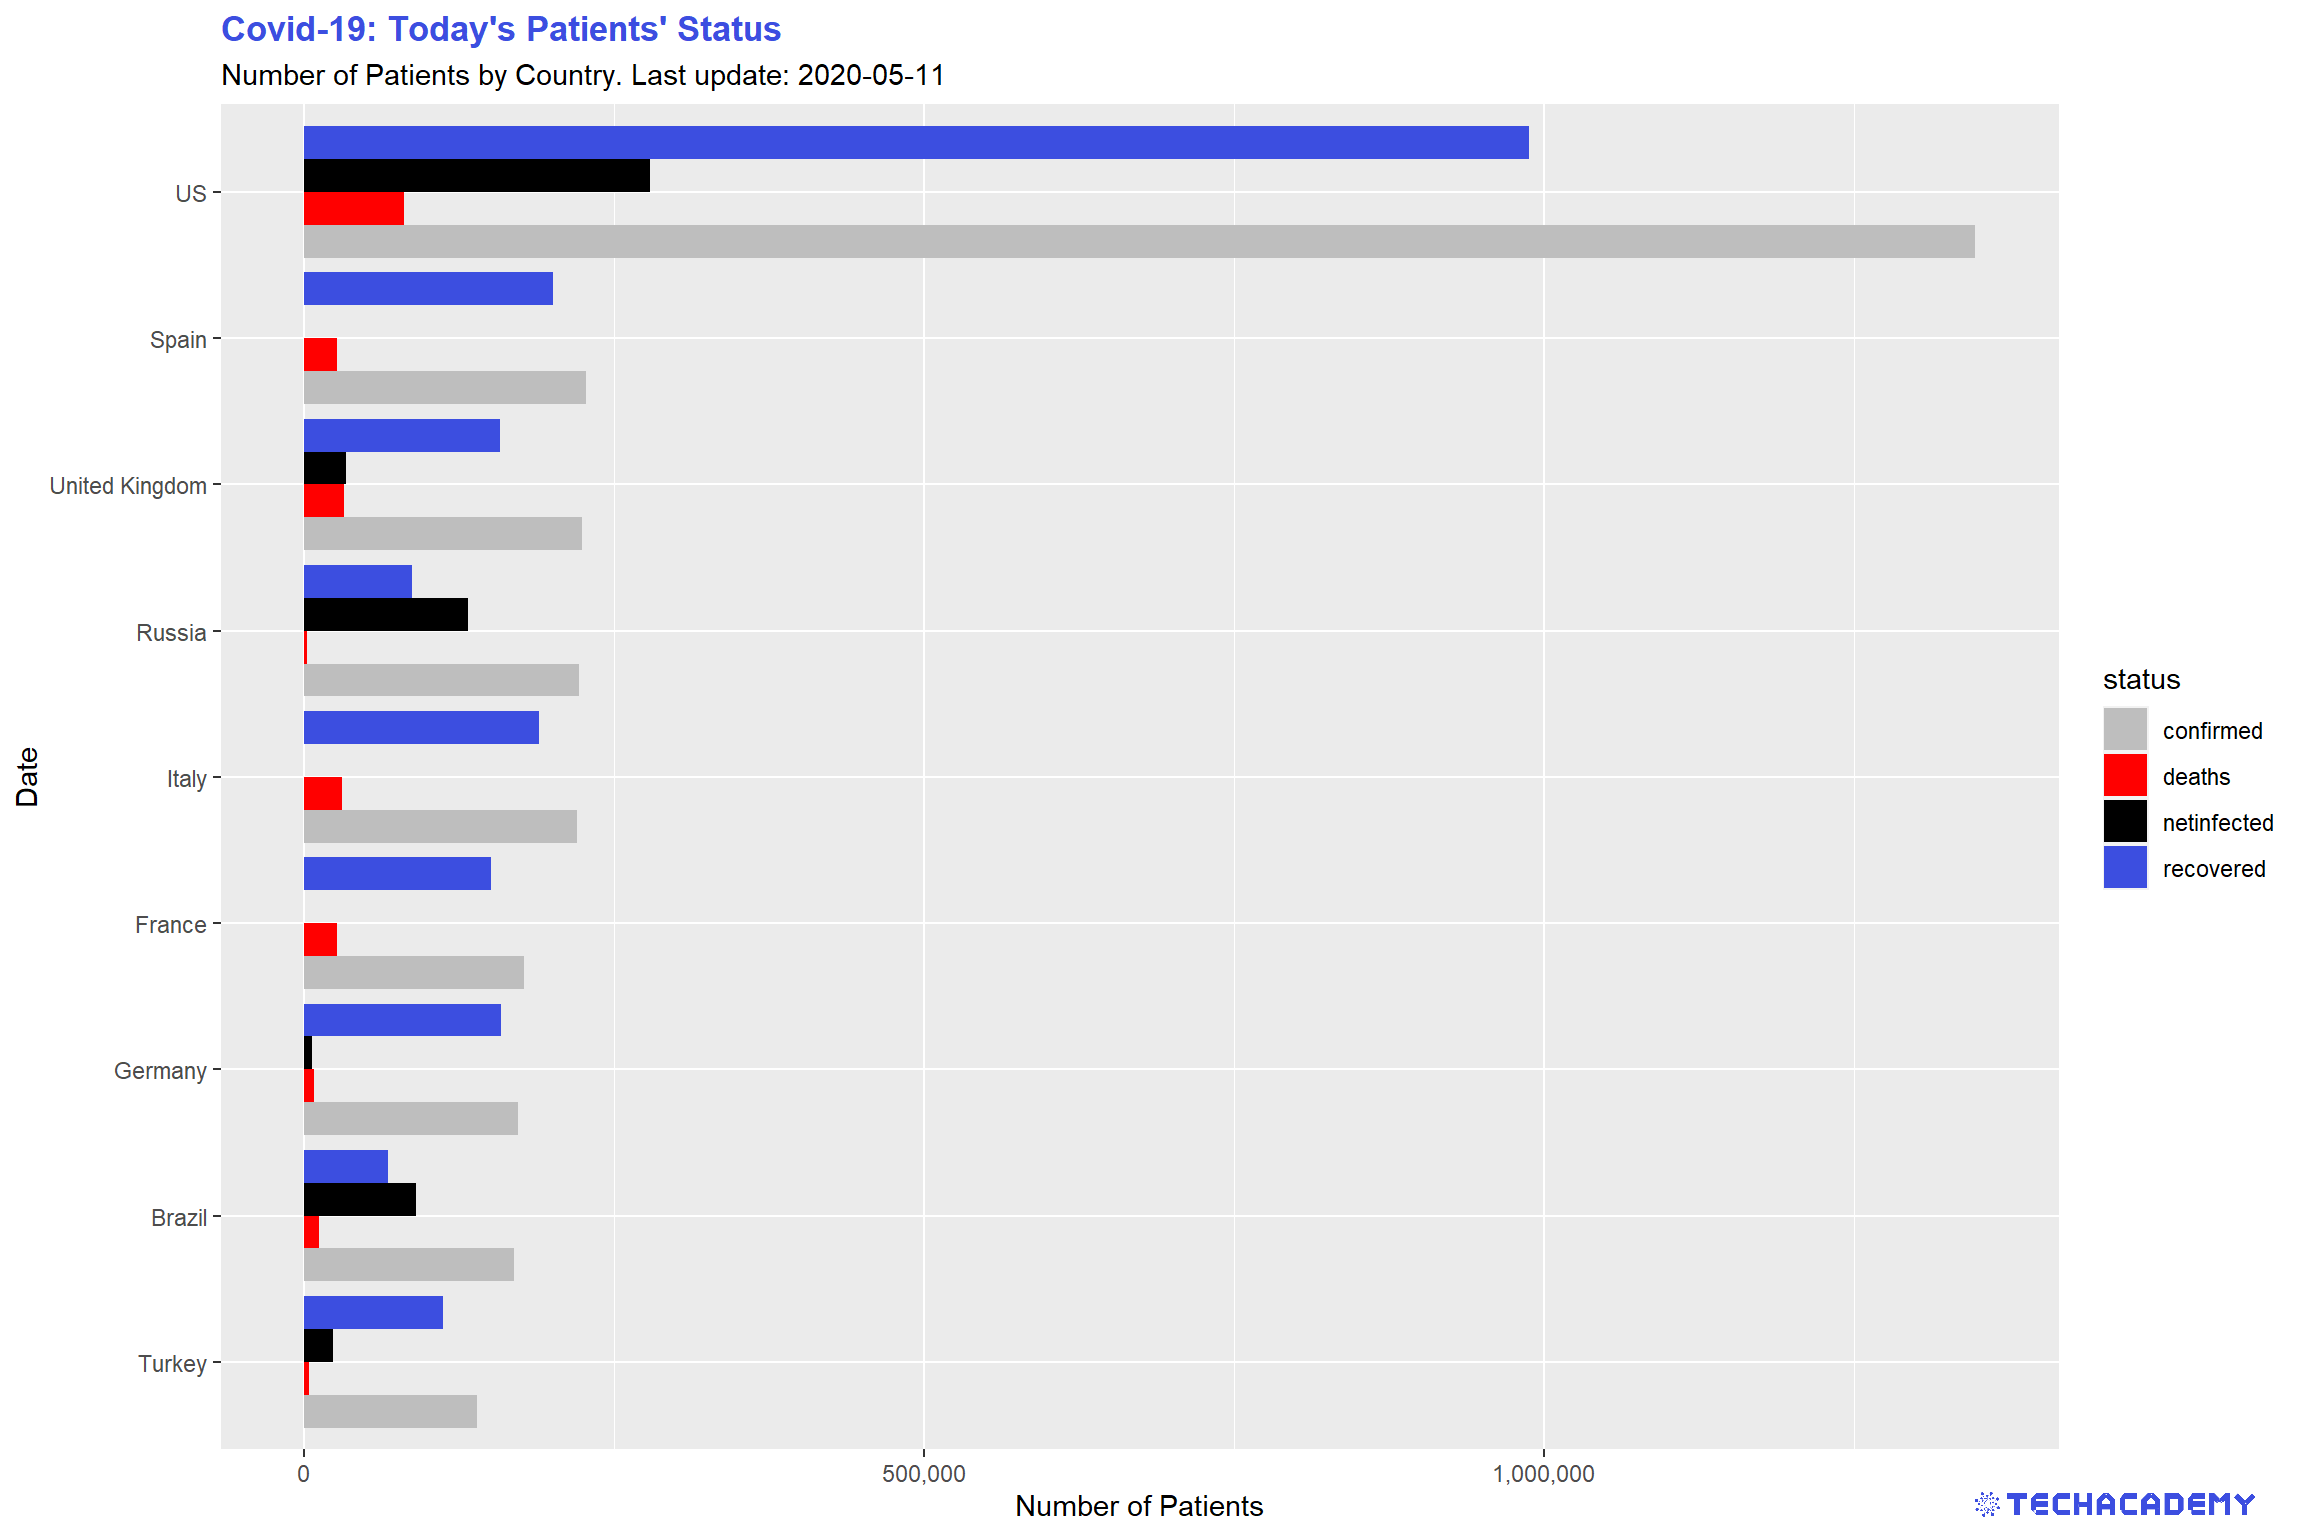
\includegraphics{output_files/figure-latex/unnamed-chunk-14-1.pdf}

\begin{tips}r

Use the same data frame and transformations from wide to long as in the last plot. Additionally, filter only the most recent snapshot by using \texttt{filter(time\ ==\ max(...))}. One of the great features of \texttt{ggplot2} is that you can easily switch from one type of plot to another one, just by changing the geom. For a barplot, use \texttt{geom\_bar} and specify its aesthetics correctly within that geom to create four different bars for each country.

You might want to flip both axes to have your barplot better structured. There is a very intuitive command to achieve that in \texttt{ggplot2}. Google yourself to the solution.

\end{tips}

\begin{tipsp}p

Use the data frame from before, i.e.~the data frame should contain at least the columns representing countries, numbers of deaths, time, net infected, and number of confirmed cases.
If you happen to have converted any column to its negative, then convert it back to positive.
Since we are not interested in the whole time series, but only in the latest data available, we can filter the data frame by the latest available date. You can use \texttt{.max()} to get the \texttt{highest} date in the appropriate column and use \texttt{df{[}df{[}‘time’{]}\ ==\ latest\_date{]}} to filter by the columns of that date.

We only want to plot nine countries with the highest number of confirmed cases: Sort by the appropriate column doing \texttt{df.sort\_values(by={[}‘...’{]},\ ascending=False)}, and then slice the data frame such that it only consists of 9 rows.

This time we are going to use pandas for plotting (which uses matplotlib's pyplot - so it is actually still creating matplotlib objects). We do so because it may be more intuitive in this case.

Our data frame should only contain the relevant columns, namely \texttt{country}, \texttt{confirmed}, \texttt{deaths}, \texttt{recovered}, and \texttt{netinfected}. You can select these columns by passing a list of column names in an indexing operator: \texttt{df{[}{[}‘col1’,\ ‘col2’,\ ...{]}{]}}. Afterwards, set the \texttt{country} column as the data frame's index.

Finally, create a figure using \texttt{plt.figure()} and plot the horizontal bars:

\begin{Shaded}
\begin{Highlighting}[]
\NormalTok{df.plot.barh(ax}\OperatorTok{=}\NormalTok{plt.gca(), width}\OperatorTok{=}\FloatTok{0.5}\NormalTok{, title}\OperatorTok{=}\NormalTok{’Best Plot Ever’, fontsize}\OperatorTok{=}\DecValTok{10}\NormalTok{)}
\end{Highlighting}
\end{Shaded}

Notice that, as already mentioned, we are using pandas' \texttt{df.plot.barh()} indestad of matplotlib's \texttt{plt.barh()} method (which we are going to use in the next exercise).
\texttt{gca()} stands for get current axes and returns the current axes instance on the current figure. If the current axes don't exist, the appropriate axes will be created. You can try to create the plot without the \texttt{ax} keyword argument and see what happens.

Don't forget to adjust/add title, labels, etc.

\end{tipsp}

\hypertarget{mortality-rate}{%
\subsubsection{Mortality Rate}\label{mortality-rate}}

Apart from the number of net infected, the mortality rate is another measure that is important for evaluating the risk of the coronavirus pandemic. Which variables would you choose to calculate the mortality rate? Would you pick deaths/confirmed cases, deaths/recovered or deaths/net infected? Choose a measure and give a reason for your decision. Then calculate a new variable for the mortality rate. In the next step, create a bar plot of the 35 countries with the highest mortality rate. Are you surprised by some countries that show up in this ranking? Is there a country with an extraordinarily high mortality rate that does not seem to make sense? Could you come up with a reason for this? Is there a way to filter the countries so that your barplot becomes more representative of the actual mortality rates?

In the next step, highlight the countries with the highest number of total confirmed cases.
The finished bar plot that has the nine countries that have the most confirmed cases highlighted should look similar to this:

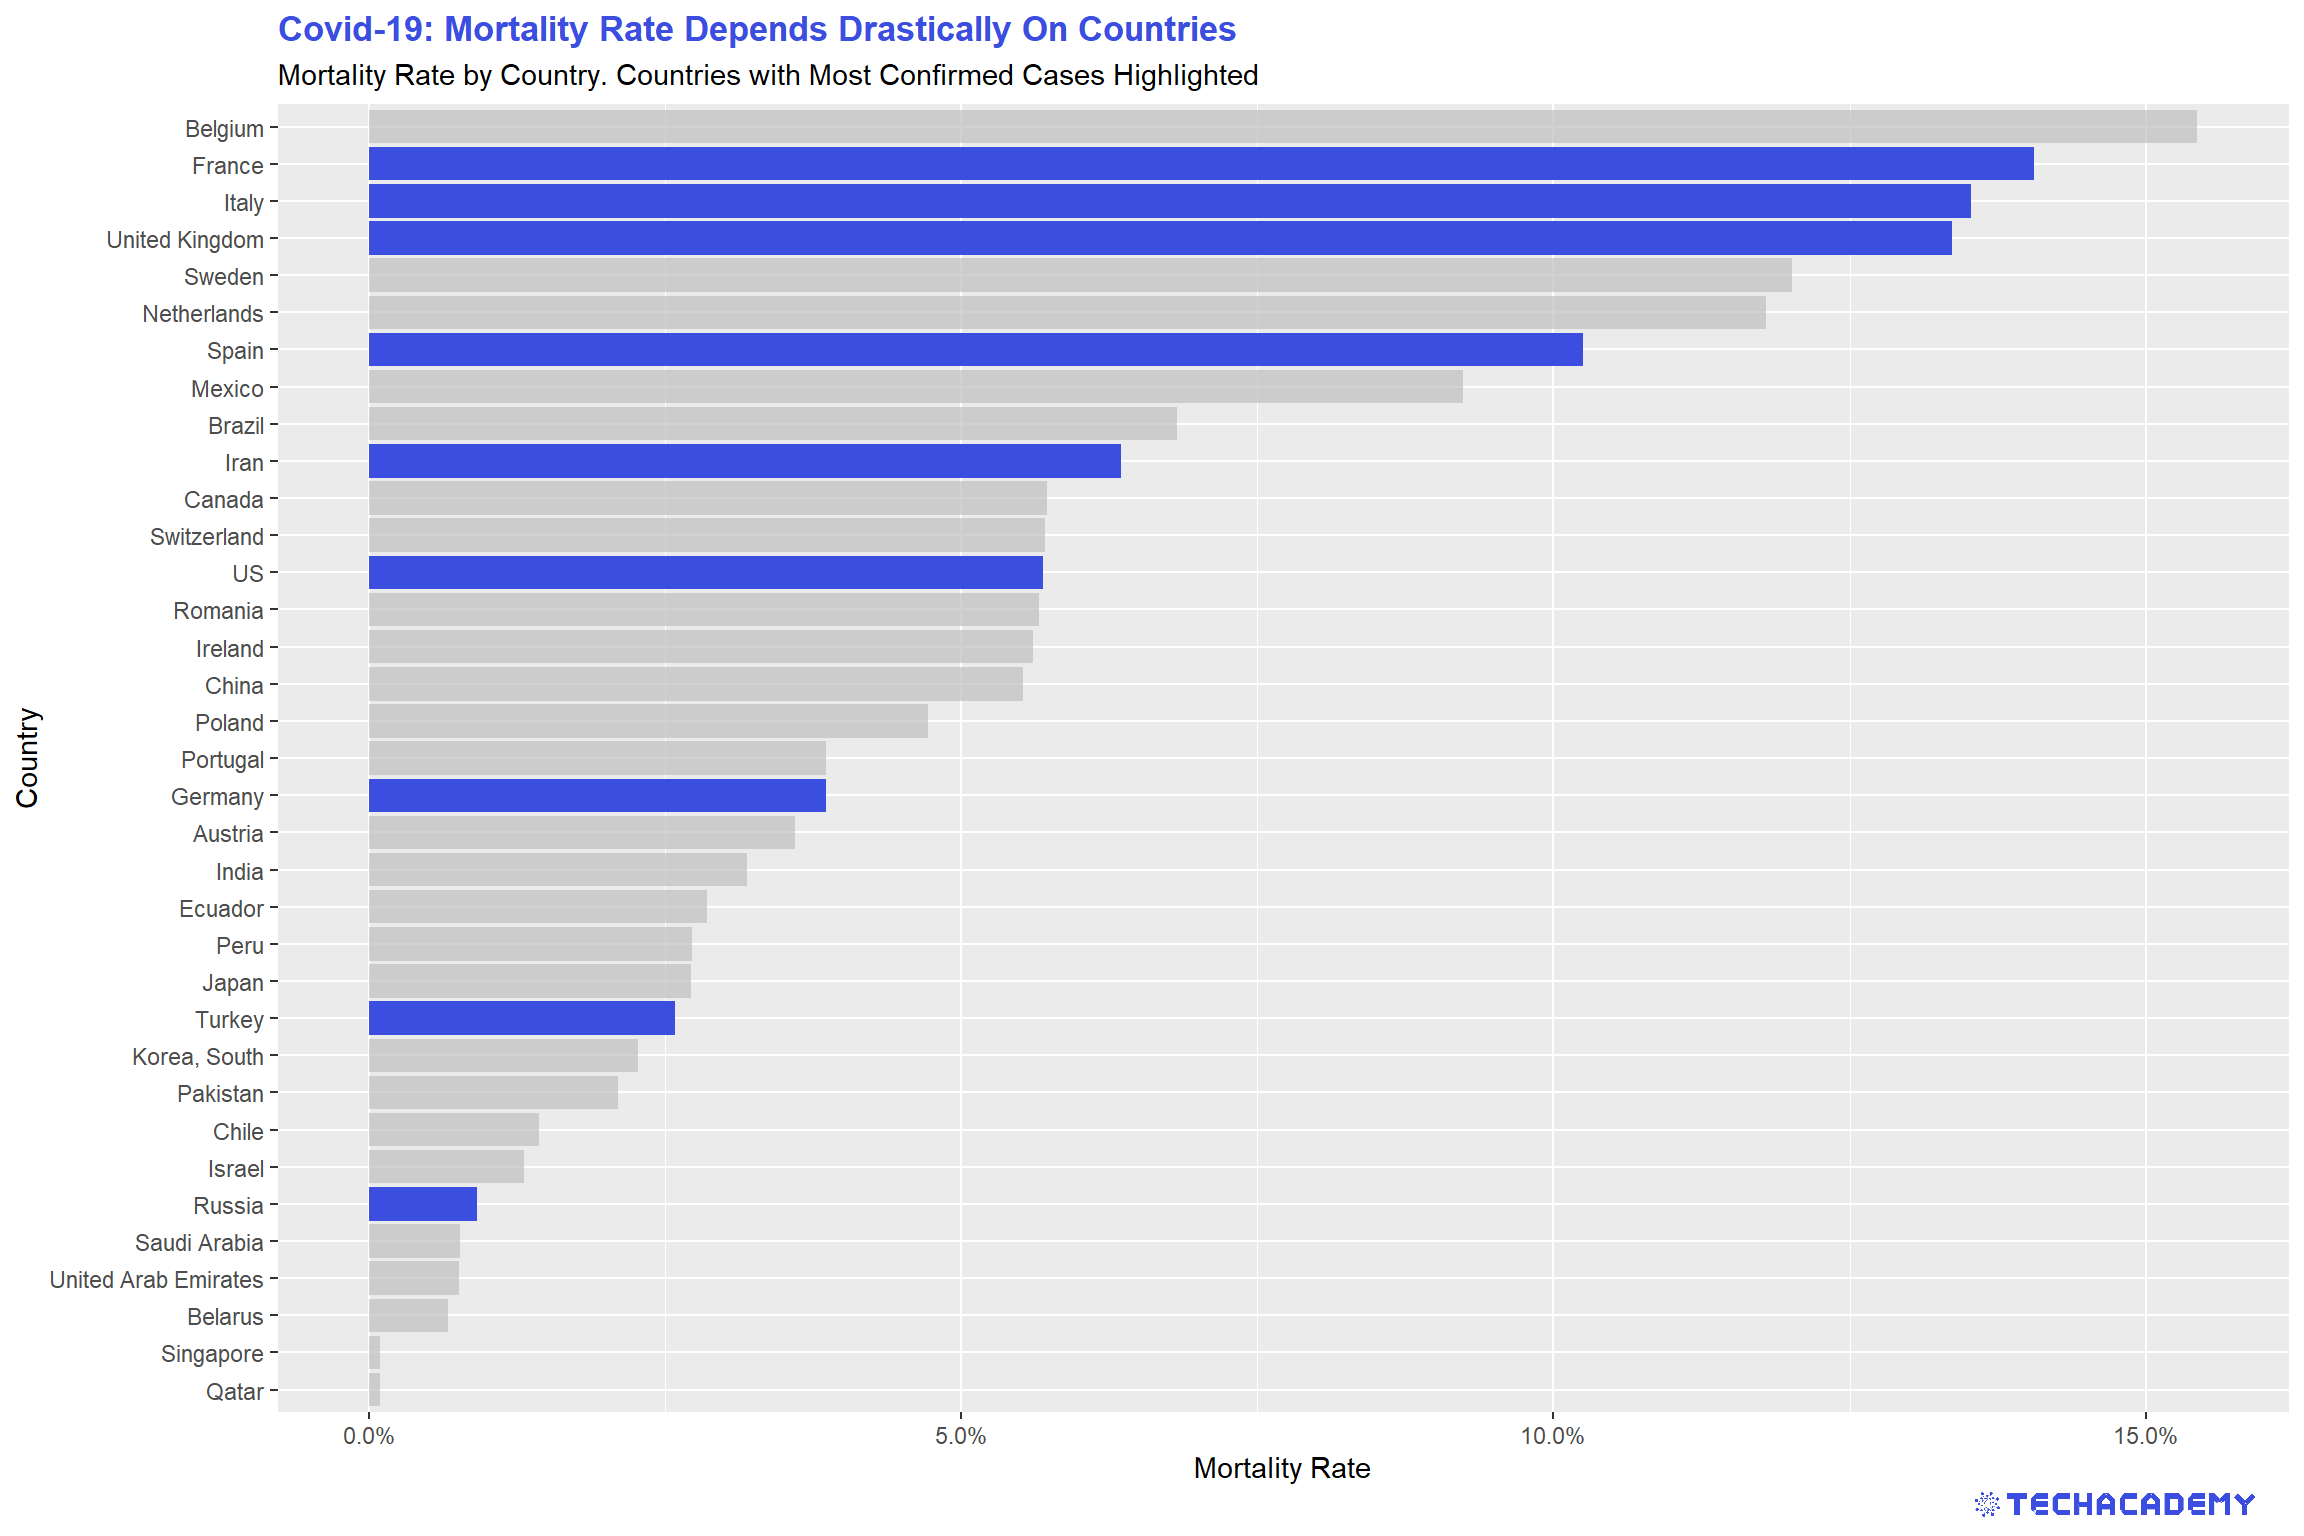
\includegraphics{output_files/figure-latex/unnamed-chunk-16-1.pdf}

Even after filtering out outliers, you can still see that there is a big difference between the countries with regard to the mortality rate. Can you explain this difference? Is it the actual mortality rate that varies between countries or is another factor at play here? What about testing? How does it affect the mortality rate?

As a Data Scientist, it is especially crucial to think about what the data tells you. Do not always take your fancy results at face value. The newly calculated mortality rate might be such a case, where you shouldn't jump to conclusions. Why do you think it is problematic to calculate the mortality rate like we did during an ongoing pandemic? If you had all the resources that you needed, how would you collect data and calculate the mortality rate? And when would you do it?

\begin{tips}r

Again, filter only the most recent snapshot by using \texttt{filter(time\ ==\ max(...))}. Now use \texttt{mutate()} to calculate the mortality rate and add it to the data frame as a new column. You already know how to do a barplot from the previous hint. You can once more use \texttt{arrange()} to order the rows in descending order -- this time by \texttt{mortality}.

To highlight certain columns of the plot, use the powerful package \texttt{gghighlight} and simply add its function for this task to your plot. Specify the countries you want to highlight as an argument. Maybe \texttt{top\_countries} from the previous sections comes in handy here?

\end{tips}

\begin{tipsp}p

The tricky part here is to highlight countries with a high number of confirmed cases.
The basic idea is to create two data frames: One with the top X countries by number of confirmed cases and another one with the top Y countries by death rate. Then iterate through each country in the second data frame (mortality rate), and see which countries can also be found in the first data frame (confirmed cases).
For countries where this is the case, we know we have to color them in a different color.

Let's start by creating those two new data frames: You can reuse the data frame that you used just before the slicing step in the last exercise and do the following:

\begin{Shaded}
\begin{Highlighting}[]
\NormalTok{highest\_confirmed }\OperatorTok{=}\NormalTok{ df\_old}
\NormalTok{highest\_mortality }\OperatorTok{=}\NormalTok{ df\_old}
\end{Highlighting}
\end{Shaded}

The first data frame should contain the top 20 (or so) countries with the highest number of confirmed cases (you need to sort and slice). We need this data frame only to determine the colors of the bars.
For the second one you need to add a new column displaying the mortality rate for each country: \texttt{df.assign(‘mortality\_rate’=\ldots{}.)}. In place of the dots, you will need to insert your formula of choice (for example you could divide the \texttt{deaths} column by the \texttt{confirmed} column). Afterwards, filter the data frame by the 35 countries with the highest mortality rate. This is the data frame that will actually be plotted.

Now we can take care of the coloring: When plotting with \texttt{plt.barh()}, matplotlib allows us to pass a list of colors as an argument, whereby the first color in that list determines the color of the first bar, the second color determines the color of the second bar, and so on. Note that the \texttt{first} bar actually corresponds to the first row in the data frame.
For example {[}`red', `red', `yellow'{]} would color the first and second bar red, but the third bar (i.e.~third row in data frame) yellow.

For us, this means that we can iterate through each country in the \texttt{highest\_mortality} data frame and check if that country is also in the \texttt{highest\_confirmed} data frame. If this is the case, we know we have to color that bar in a different color:

\begin{Shaded}
\begin{Highlighting}[]
\NormalTok{cols }\OperatorTok{=} \BuiltInTok{list}\NormalTok{()  }\CommentTok{\# initiate empty list}
 
\ControlFlowTok{for}\NormalTok{ country }\KeywordTok{in}\NormalTok{ highest\_mortality[‘country’]:}
    \CommentTok{\# if country also in highest\_confirmed, then highlight in blue}
    \ControlFlowTok{if}\NormalTok{ country }\KeywordTok{in}\NormalTok{ highest\_confirmed[‘country’].values:}
\NormalTok{        cols.append(‘blue’)}
    \ControlFlowTok{else}\NormalTok{:}
\NormalTok{        cols.append(‘grey’)}
\end{Highlighting}
\end{Shaded}

Again, understand that the first color in the \texttt{cols} list determines the color of the first bar (i.e.~the first row, or country, in our data frame).
Can you create the color list in one line making use of python's list comprehension?

Now, everything is ready to be plotted with \texttt{plt.barh(highest\_mortality{[}‘country’{]},\ highest\_mortality{[}’mortality\_rate’{]},\ color=cols)}.

\end{tipsp}

\hypertarget{visualization-with-maps}{%
\subsection{Visualization with Maps}\label{visualization-with-maps}}

This part will be the final and most advanced part of the EDA -- but also the most rewarding. If you have ever checked the news during the coronavirus outbreak you must have come across a world map with information of how the virus is spreading and how badly each country is affected. You will now build your own map where you can show which countries are affected and how high the number of confirmed cases is. Instead of having to rely on others' decisions regarding the visualization of data on the virus, by creating your own map you can decide freely which type of maps visualization you prefer and which information you want to highlight.

You already have coordinates included in your data set but some data transformation is still necessary. It can get a little tricky, but as before we will give you hints along the way so that you will have an idea of what to do.

Up until this point the basic ideas of the tasks were the same for the Python and R track so the introduction to the exercises was the same, but for the maps tasks, the output will vary significantly between the tracks. That is why you will find every information necessary as well as the output you are working towards in the respective track boxes.

\hypertarget{color-countries-by-confirmed-cases}{%
\subsubsection{Color Countries by Confirmed Cases}\label{color-countries-by-confirmed-cases}}

\begin{tips}r

For this section, we've already prepared a new data set. Load \texttt{world\_map.csv} into your workspace and have a look at the included variables. It contains all data to draw all countries' borders on a map. Also, we've merged the Covid-19 data on a single day to the spatial data.

We will start with a basic map that shows all countries on a world map and colors them according to the number of confirmed cases. How convenient that we can also use our favorite graphics package \texttt{ggplot2} for that task. Supply the plot's aesthetics with the longitude and latitude as x and y-coordinates, respectively. Additionally, every country is identified by a unique \texttt{group}. We need to supply this to the aesthetics as well by \texttt{aes(...,\ group\ =\ group)} such that the function knows which data points belong to the same country. As geom, we will use \texttt{geom\_polygon()} to draw the borders. Use the argument \texttt{fill\ =\ ...} to determine the color of a country based on \texttt{confirmed}.

A problem you will run into with this technique of map generation is that the plot will be distorted if you change its size. Countries will become wider or longer than you might be used to when looking at a typical map. This issue is connected to the broader challenge of projecting areas on a ball (the earth) from a 3D element to a simple 2D map. Check online how you can handle the proper projection in \texttt{ggplot2} and implement that in your map.

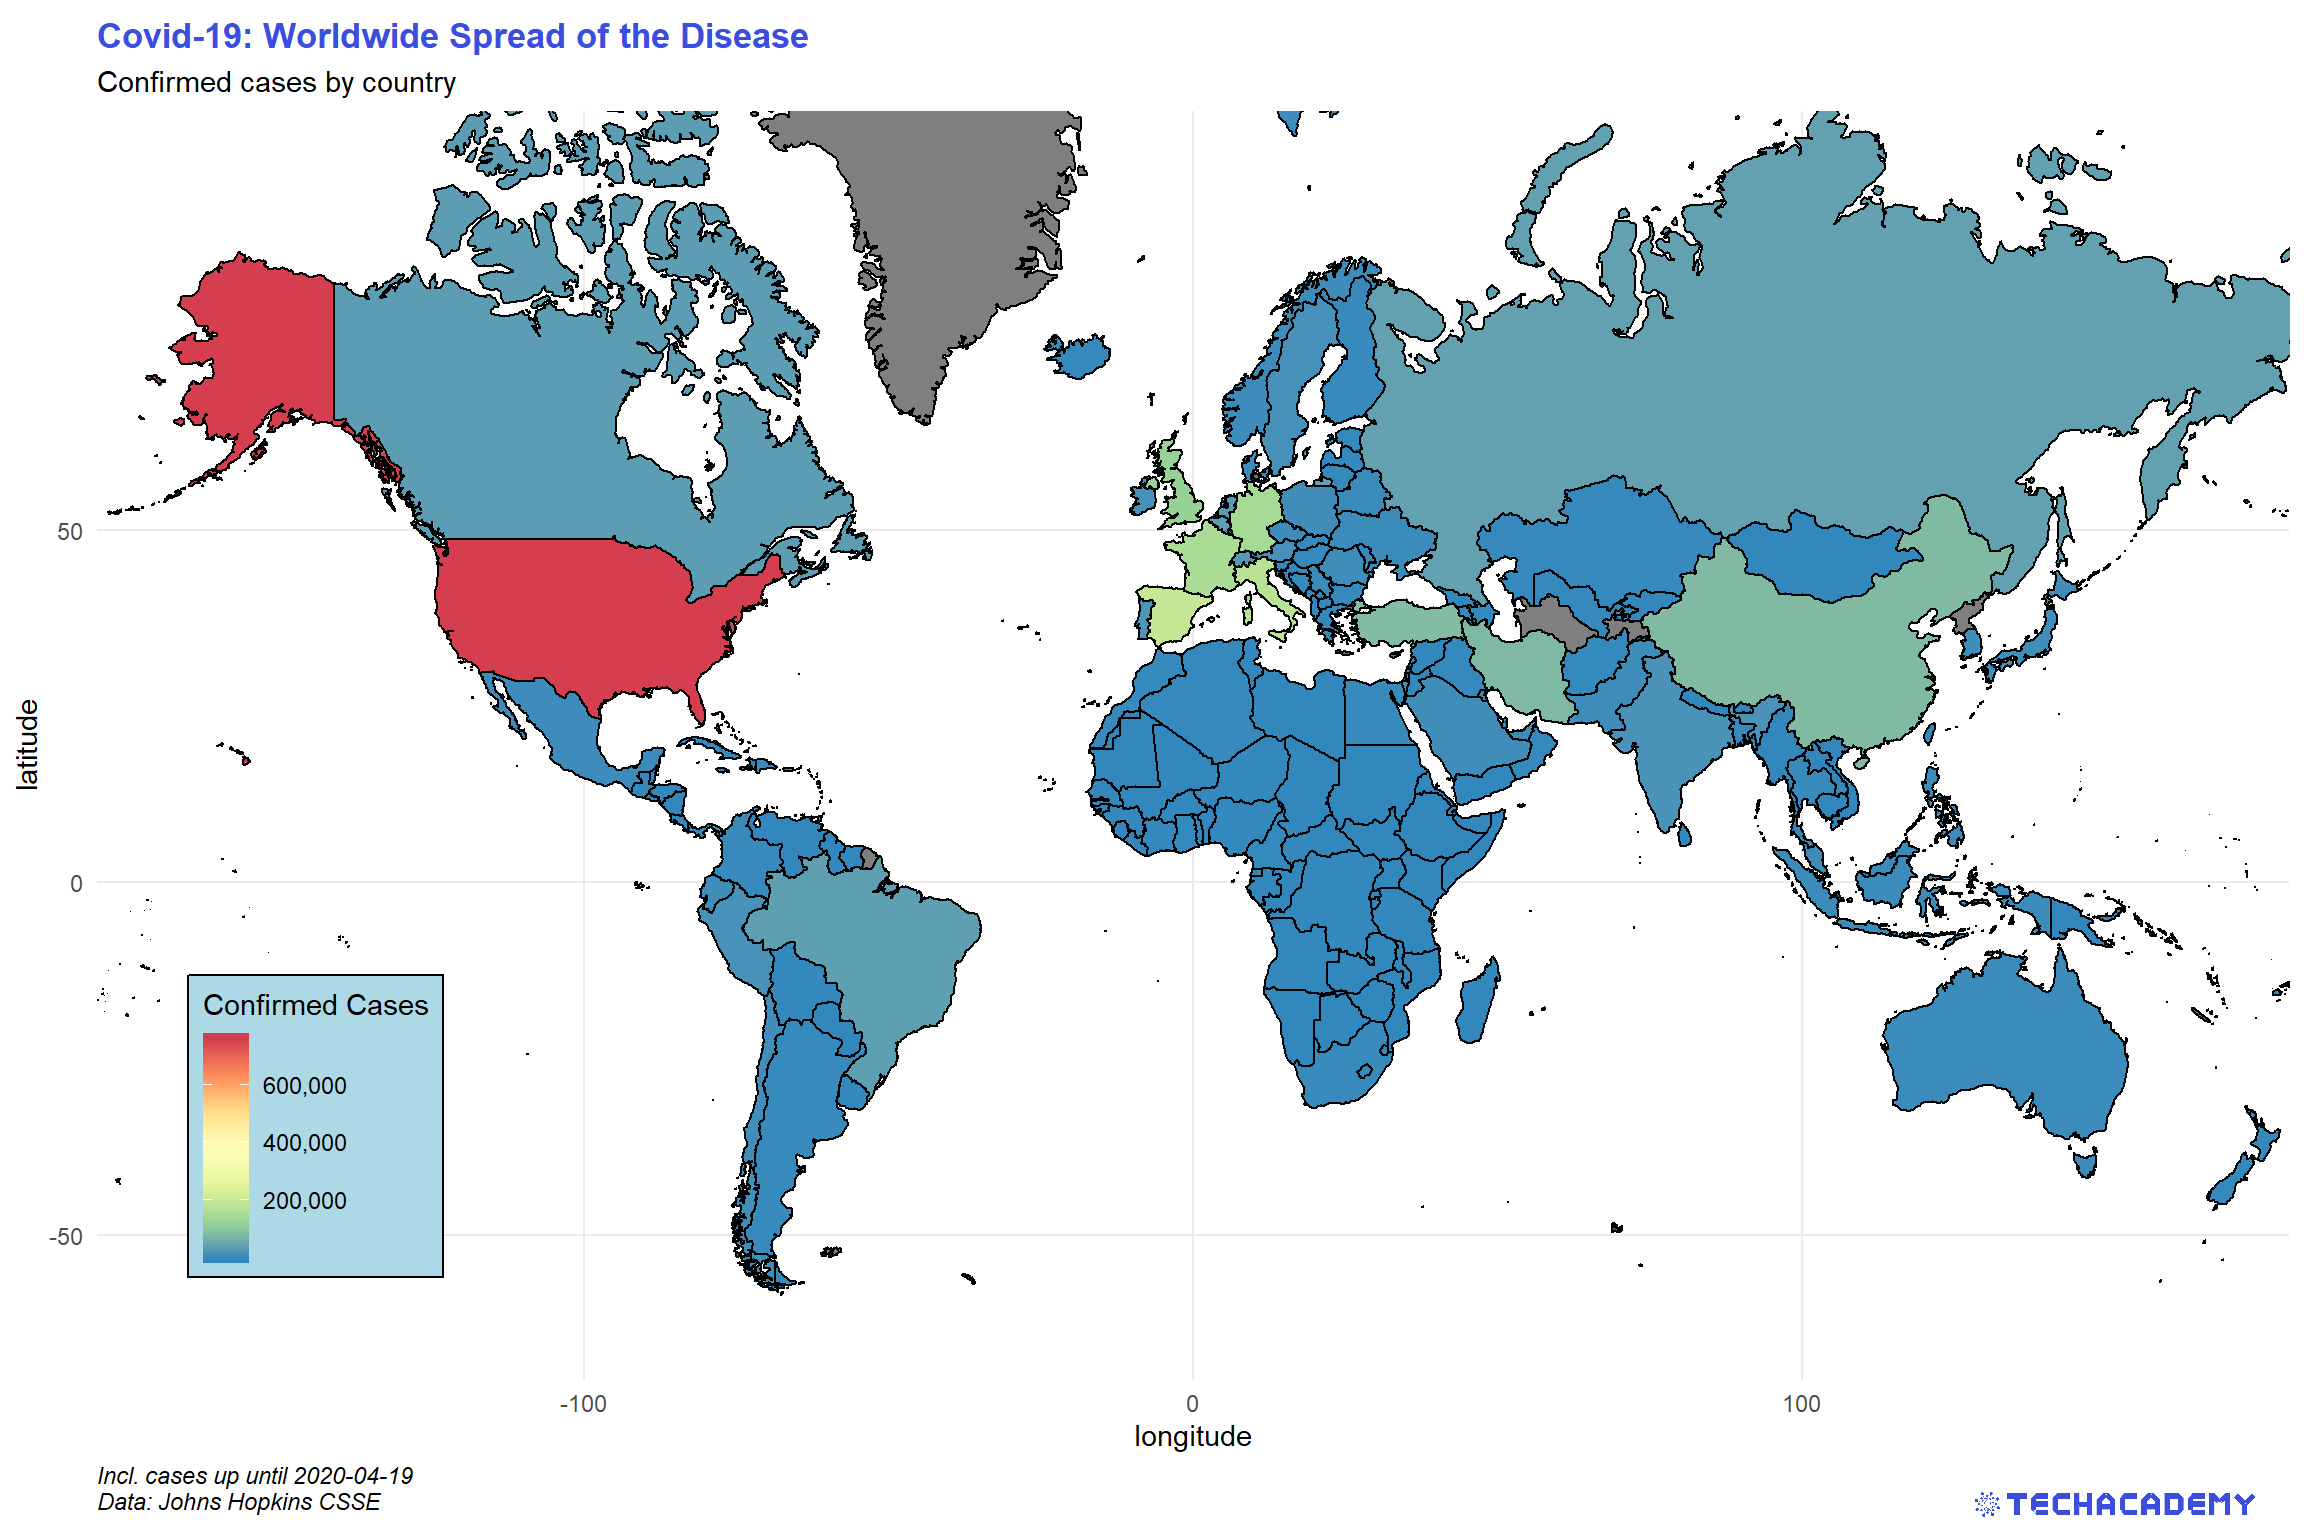
\includegraphics{output_files/figure-latex/unnamed-chunk-19-1.pdf}

\end{tips}

\begin{tipsp}p

As a first step, we want to visualize the outbreak in each country with circles, where each country's circle size is is dependent on the amount of confirmed cases.

Let's start by importing the familiar \texttt{confirmed.csv} file.
The goal of our map is to inform the viewer about the number of confirmed cases per country for the latest date available: Find out the latest date and filter the data frame by that date.

Filter the data frame by the columns of interest to facilitate the iteration over each row. The columns are: \texttt{country}, \texttt{latitude}, \texttt{longitude}, and \texttt{confirmed}.
Now that our data frame is in the right format, it is time to check out the documentation of the \href{https://ipyleaflet.readthedocs.io/en/latest/}{ipyleaflet library}. This is the library we will use to create our maps.

For our first map, we will use the module ``Circle Marker''. Please be sure to take a look at the example in the documentation before proceeding, especially for knowing which modules you need to import!

If you copy-paste-run the example in the docs, you can see that it plots only one single circle on the map -- but we want multiple circles!

Let's start by making sure that when creating the instance \texttt{m} of the \texttt{Map} class you pass the positional argument \texttt{center=(48,\ -2)} (which might differ from the example in the documentation):

\begin{Shaded}
\begin{Highlighting}[]
\NormalTok{m }\OperatorTok{=}\NormalTok{ Map(center}\OperatorTok{=}\NormalTok{(}\DecValTok{48}\NormalTok{, }\OperatorTok{{-}}\DecValTok{2}\NormalTok{), zoom}\OperatorTok{=}\DecValTok{9}\NormalTok{, basemap}\OperatorTok{=}\NormalTok{basemaps.CartonDB.Positron)}
\CommentTok{\# Feel free to change the zoom and layout of the basemap.}
\end{Highlighting}
\end{Shaded}

In order to plot multiple circles, you may want to iterate through every row in your data frame. Doing so, you will find it helpful to use the following technique:

\begin{Shaded}
\begin{Highlighting}[]
\ControlFlowTok{for}\NormalTok{ i, country, }\BuiltInTok{long}\NormalTok{, lat, nr }\KeywordTok{in}\NormalTok{ confirmed\_df.itertuples(index}\OperatorTok{=}\VariableTok{True}\NormalTok{):}
    \ControlFlowTok{pass}  \CommentTok{\# your for{-}loop body here}
\end{Highlighting}
\end{Shaded}

In each iteration you would need to create an instance of the \texttt{CircleMarker} class.
Additionally, call the methods \texttt{.location()}, \texttt{.radius()}, \texttt{.color()}, and \texttt{.fill\_color()} and pass on the right arguments. In the same iteration call the \texttt{.add\_layer()} method with the above instance of the \texttt{CircleMarker} as its argument.

Note: Think about a way to roughly size the circles, such that the viewer has an idea about the number of cases in each country listed in our data. Obviously, if you just set the number of confirmed cases as the radius, the circles are going to look way too big. Maybe use something like the logarithm of that number?

It probably won't look great on your first try -- just give it another shot!

\end{tipsp}

\begin{tipsp}p

This is what your map could look like:

\begin{center}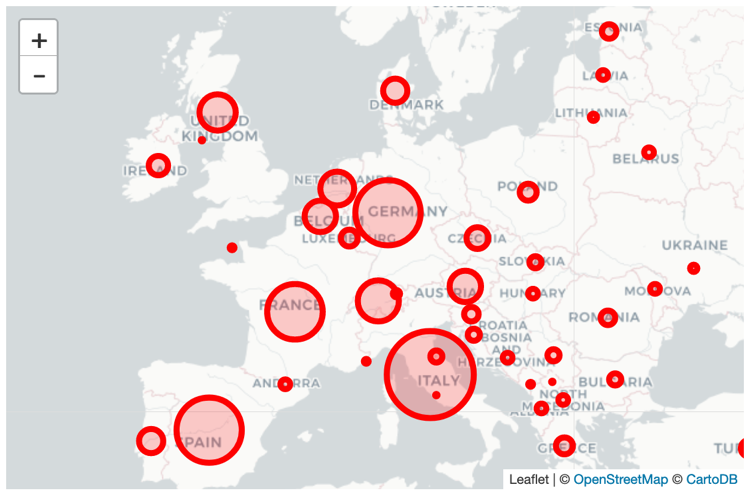
\includegraphics[width=1\linewidth]{plots/p-map-circle} \end{center}

\end{tipsp}

\hypertarget{enhance-your-map}{%
\subsubsection{Enhance Your Map}\label{enhance-your-map}}

\begin{tips}r

The next map will be the most advanced one -- plot all European countries, color them according to the number of deaths and draw a label that states the number of deaths in that country. First, extract the \texttt{countrycode} of all countries within Europe. We provide you with a country lookup table that defines the region (e.g.~Europe) for every individual country. Import this data set and extract the desired country codes into a vector. Use this structure:

\begin{Shaded}
\begin{Highlighting}[]
\NormalTok{country\_lookup \textless{}{-}}\StringTok{ }\KeywordTok{read.csv}\NormalTok{(}\StringTok{"your/path/country\_lookup.csv"}\NormalTok{, }\DataTypeTok{stringsAsFactors =}\NormalTok{ T)}
\NormalTok{country\_lookup }\OperatorTok{\%\textgreater{}\%}\StringTok{ }
\StringTok{  }\KeywordTok{filter}\NormalTok{(region }\OperatorTok{==}\StringTok{ }\NormalTok{“}\OperatorTok{\textless{}}\ErrorTok{\textless{}}\NormalTok{specify region here}\OperatorTok{\textgreater{}}\ErrorTok{\textgreater{}}\NormalTok{”) }\OperatorTok{\%\textgreater{}\%}
\StringTok{  }\CommentTok{\# in case you want to exclude more countries, filter them here         }
\StringTok{  }\KeywordTok{pull}\NormalTok{(alpha}\FloatTok{.3}\NormalTok{) {-}\textgreater{}}\StringTok{ }\NormalTok{countrycode\_europe}
\end{Highlighting}
\end{Shaded}

Now you want to calculate the geographic center of a country. This will help you to place the label on the country later on. Generate that data set with the following hints:

\begin{Shaded}
\begin{Highlighting}[]
\NormalTok{world\_map }\OperatorTok{\%\textgreater{}\%}\StringTok{ }
\CommentTok{\# group and summarize the variables of interest here  }
\CommentTok{\# filter your data frame to only have the relevant countries}
\StringTok{  }\KeywordTok{filter}\NormalTok{(countrycode ...) }\OperatorTok{\%\textgreater{}\%}
\CommentTok{\# create column with labels:}
\CommentTok{\# Use “\textbackslash{}n” within a string as a line break between }
\CommentTok{\# the country name and the number of confirmed cases}
\CommentTok{\# generate a new variable that contains the label in a string format}
\CommentTok{\# then assign everything to a new data frame in the last line}
\NormalTok{... {-}\textgreater{}}\StringTok{ }\NormalTok{label\_centroids}
\end{Highlighting}
\end{Shaded}

Now you can generate a map in the same way as in the first maps exercise. Filter all European countries from \texttt{world\_map} using \texttt{countrycode\_europe}. After adding the polygons, use the package \texttt{ggrepel} and its function \texttt{geom\_label\_repel()} to draw the labels. Provide the required argument(s), and define aes(\ldots) differently than in geom\_polygon(). Hint: use your newly generated data frame \texttt{label\_centroids}. It is important to set \texttt{inherit.aes\ =\ FALSE}, otherwise \texttt{ggplot2} inherits the aesthetics from the geom before.

Now enhance the appearance of your plot by defining another color scale for the countries. Just having different shades of blue is not that helpful for distinguishing the countries.

\end{tips}

\begin{tips}r

This is what your map could look like:

\begin{center}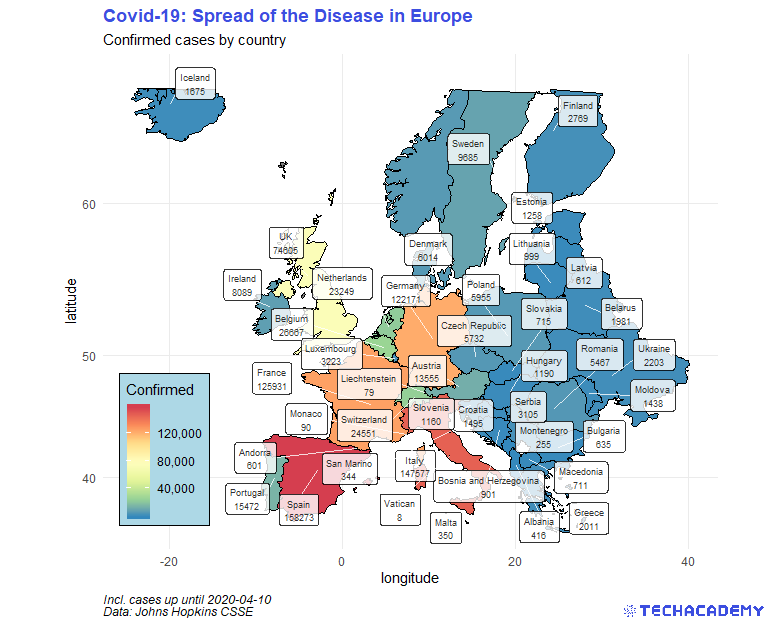
\includegraphics[width=1\linewidth]{plots/r-map-label} \end{center}

\end{tips}

\begin{tipsp}p

For our last map, we are going to create a world map and color each country by its number of confirmed cases.
You should be able to use the data frame for confirmed cases from before. But before continuing, you may want to have a look at the ipyleaflet documentation for the layer \texttt{GeoJson}, which we are going to use here.

In contrast to before, when we only needed latitude and longitude for a country to place our circles, we now need all the coordinates of each country's border to be able to draw it.
Thus, we've prepared a \texttt{.json} file for you with all border coordinates (i.e.~country polygons) for each country, which is stored as \texttt{geo.json}.
You can load \texttt{.json} files into your jupyter notebook doing:

\begin{Shaded}
\begin{Highlighting}[]
\ControlFlowTok{with} \BuiltInTok{open}\NormalTok{(‘}\OperatorTok{/}\NormalTok{PATH}\OperatorTok{/}\NormalTok{TO}\OperatorTok{/}\NormalTok{geo.json’, ‘r’) }\ImportTok{as}\NormalTok{ f:}
\NormalTok{    world\_map\_dict }\OperatorTok{=}\NormalTok{ json.load(f)}
\end{Highlighting}
\end{Shaded}

This file contains a ton of data. Just notice that each list element in the dictionary key \texttt{features} contains the name of the country, as well as its coordinates (for example print \texttt{world\_map\_dict{[}\textquotesingle{}features\textquotesingle{}{]}{[}0{]}}).

In order to use the confirmed cases data frame for this map, we need to convert it into a dictionary with country names as keys and the respective number of confirmed cases as its values. We can achieve this in one line with dict comprehension and python's built in zip function: \texttt{dict(zip(df.country,\ df.confirmed))}.

Now that we have our \texttt{confirmed\ cases} and the \texttt{borders} dictionaries, we may now take care of the coloring.
Again, we already prepared a json file called \texttt{colors.json}. Looking at its content in your Jupyter notebook, you will see that it has numbers stored as keys, and rgb-color-codes stored as the respective values. The numbers are actually the number of confirmed cases to which the colors ``belong'' to.
\texttt{ipyleaflet} requires us to make two lists out of this dictionary, because we need to pass both as separate arguments when instantiating the map's \texttt{layer}.
You can create both lists in two lines using python's list comprehension:

\begin{Shaded}
\begin{Highlighting}[]
\NormalTok{color\_list }\OperatorTok{=}\NormalTok{ [v }\ControlFlowTok{for}\NormalTok{ k,v }\KeywordTok{in}\NormalTok{ color\_codes.items()]}
\NormalTok{nr\_list }\OperatorTok{=}\NormalTok{ [}\BuiltInTok{float}\NormalTok{(k) }\ControlFlowTok{for}\NormalTok{ k,v }\KeywordTok{in}\NormalTok{ color\_codes.items()]  }
\end{Highlighting}
\end{Shaded}

\end{tipsp}

\begin{tipsp}p

Notice how we had to use python's float method to convert the numbers to float, as they were stored as strings in our colors.json file.

That's pretty much it! We can now create the \texttt{layer}-instance of the Choropleth class:

\begin{Shaded}
\begin{Highlighting}[]
\NormalTok{layer }\OperatorTok{=}\NormalTok{ ipyleaflet.Choropleth(}
\NormalTok{    geo\_data}\OperatorTok{=}\NormalTok{world\_map\_dict,}
\NormalTok{    choro\_data}\OperatorTok{=}\NormalTok{confirmed\_dict,}
\NormalTok{    colormap}\OperatorTok{=}\NormalTok{LinearColormap(colors}\OperatorTok{=}\NormalTok{color\_list, index}\OperatorTok{=}\NormalTok{nr\_list,}
\NormalTok{                            vmin}\OperatorTok{=}\DecValTok{0}\NormalTok{, vmax}\OperatorTok{=}\NormalTok{nr\_list[}\OperatorTok{{-}}\DecValTok{1}\NormalTok{]),}
\NormalTok{    border\_color}\OperatorTok{=}\StringTok{\textquotesingle{}black\textquotesingle{}}\NormalTok{,}
\NormalTok{    style}\OperatorTok{=}\NormalTok{\{}\StringTok{\textquotesingle{}fillOpacity\textquotesingle{}}\NormalTok{: }\FloatTok{0.8}\NormalTok{, }\StringTok{\textquotesingle{}dashArray\textquotesingle{}}\NormalTok{: }\StringTok{\textquotesingle{}5, 5\textquotesingle{}}\NormalTok{\})}
 
\NormalTok{m }\OperatorTok{=}\NormalTok{ Map(center}\OperatorTok{=}\NormalTok{(}\DecValTok{43}\NormalTok{, }\DecValTok{0}\NormalTok{), zoom}\OperatorTok{=}\DecValTok{4}\NormalTok{)}
\NormalTok{m.add\_layer(layer)}
\NormalTok{m}
\end{Highlighting}
\end{Shaded}

Feel free to play around with the maps you created. Maybe try to insert some controls (see under \texttt{controls} in the ipyleaflet documentation), like the zoom-bar you can see in the picture below, or a full screen button.

This is how your map could look like:

\begin{center}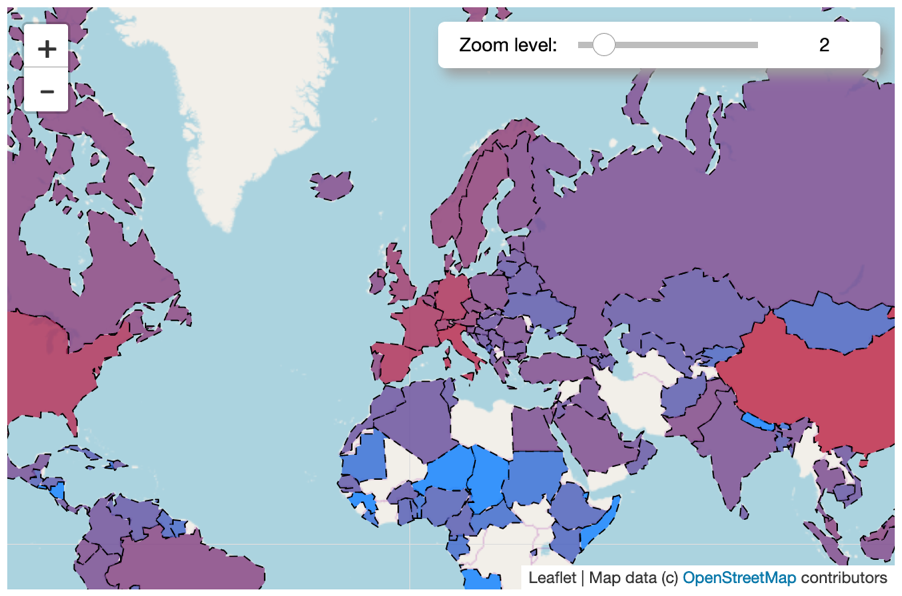
\includegraphics[width=1\linewidth]{plots/p-map-color} \end{center}

\end{tipsp}

Congratulations! Because you put in the effort and determination you managed to perform data transformations as well as visualization techniques that are highly relevant for modern Data Science. You can proudly say that you now have acquired basic skills in the field of Data Science by successfully completing the first part of the project. If you are part of the beginner track you have fulfilled the necessary requirements. However, we do recommend that you have a look at the second part of the project and try and solve it as well. This is the part where it really gets interesting because we will have a look at methods of predicting the future. Sounds exciting? Then get ready!

\newpage

\hypertarget{covid-19-prediction}{%
\section{Covid-19 Prediction}\label{covid-19-prediction}}

Until now you have looked deeply into the given data and visualized different aspects of it. But wouldn't it be nice to predict the number of new infections with other variables contained in the data set? In this part, we'll do just that and go a step further by developing simple (or more advanced) statistical models which will be able to predict the amount of new infections on a given day.

These predictions will be based on features which contain information about this specific day. The goal of our analysis will be to identify dependencies (correlations) between these features and the number of new infections. Your model can then exploit those correlations to make predictions.

You already looked at the number of Google search queries for ``corona''-related keywords in the first part. Do you think that those might have something in common with the daily new infections? Also, you've analyzed stock market data for the relevant period. Is the stock market moving according to new infections? You might think that those two variables have some predictive power. When a person is showing symptoms and fears that they might have contracted the disease, they will google it and try to get more information. Also, the more new infections are announced, the worse for the economy and hence -- as a proxy for general economic expectations -- the stock market. In this part, we'll check those claims and see how well models based on those and other variables perform.

The procedure to get to a statistical model ready for prediction is divided into two parts. First, you train your model on some data which is called the \textbf{train} data set. Afterwards, you test your model on data which the model has never come into contact with during training. This is called the \textbf{test} data set.
This procedure gives us a good estimation of how well your model would perform in real life with completely new data.
If you train your model in a way that it only remembers the data from the training data set, it would perform very well on this set. However, it would not be able to generalize the structure of the data and transfer it to new unseen data -- this problem is called \emph{overfitting}. We can detect it by evaluating the predictions of our model on a test data set. On the other hand, you could also \emph{underfit} your model. This means it doesn't learn the relationships between the dependent and independent variable(s) well enough to perform reasonably well on the unseen test data set. Hence, your top priority must be to find the optimal balance between those two problems and fit your model well to both training and test data.

But how can you check if your model under- or overfitted or whether it is just fine? As already explained above, after the training process we evaluate our model by seeing how well it performs when being used on the test data set. We do this by letting our model use the previously unseen test observations to make predictions for the dependent variable. In our case, we would use the Google trends variable of the test data set to predict the number of new infections. We then compare our predictions with the actual number of cases that is contained in the test data set and see how close we came.

For this performance evaluation it is useful to define a metric which compares the prediction of your model with the true values. One such measure is the \emph{mean absolute percentage error (MAPE)} which computes the mean percentage deviation of the prediction from the true values.

\[ MAPE = \frac{1}{n} \sum_{t=1}^n \left\lvert\frac{(y_t - \hat{y}_t)}{y_t}\right\rvert \]

The larger the MAPE is, the worse your model performs. You can interpret that metric as the average percentage deviation of your model's prediction to the true values. \(MAPE = 0.5\) for example means that on average, your prediction is 50\% off the true values. If you look closer at other prediction tasks for continuous variables, you'll also come across some other metrics such as the \emph{root mean squared error (RMSE)} or \emph{mean absolute error (MAE)}. Think about why those are not well suited for this kind of prediction evaluation.

So let's get started with the prediction. Once again, we have to lay some groundwork before we can let our models do the magic. You'll start with some feature engineering and correlation analysis. After that, you can set up your first very simple univariate linear regression model (i.e.~one dependent and one independent variable) for a limited set of observations -- in this case German data only. When we've got that running, we'll continuously improve our model by adding or modifying features. We then take our best model and check out how well it performs on the entire data set. You'll then see how well the German model runs on four other countries.

\hypertarget{feature-engineering-and-correlation-analysis}{%
\subsection{Feature Engineering and Correlation Analysis}\label{feature-engineering-and-correlation-analysis}}

Before we start, you'll need to load a new data set. We've already prepared a panel data set with five countries and many important characteristics. Import \texttt{predict.csv}, on which this entire part will be based. Many variables are similar to the data set before, but there are also some important differences.
The goal of our model is to predict the number of new infections per day. This value corresponds to the difference between the cumulative number of infections of the current day and the day before in each country. Assign the computed values to a new variable \texttt{new\_confirmed} -- this will be the column your model is trying to predict.
In a later model, we also want to include \texttt{lags} for the Google Search trend data. This means that each row of our data frame should not only contain the search trend for the current day but also from the day before (lag=1), two days before (lag=2) and so on. Compute the lags from 1 to 10 for each row and assign it to new columns in your data frame. We will explain later why we need this and what the idea behind this feature is, but it is easier to compute it right away.

The next step is to analyse the dependency between the different columns or features in your train data set. Select several columns of the data frame, compute the correlations between them and visualize them in a scatterplot. It is important to include the column \texttt{new\_confirmed} here because we are especially interested in the dependency between the other features and this column.

Your output could look similar to this one:

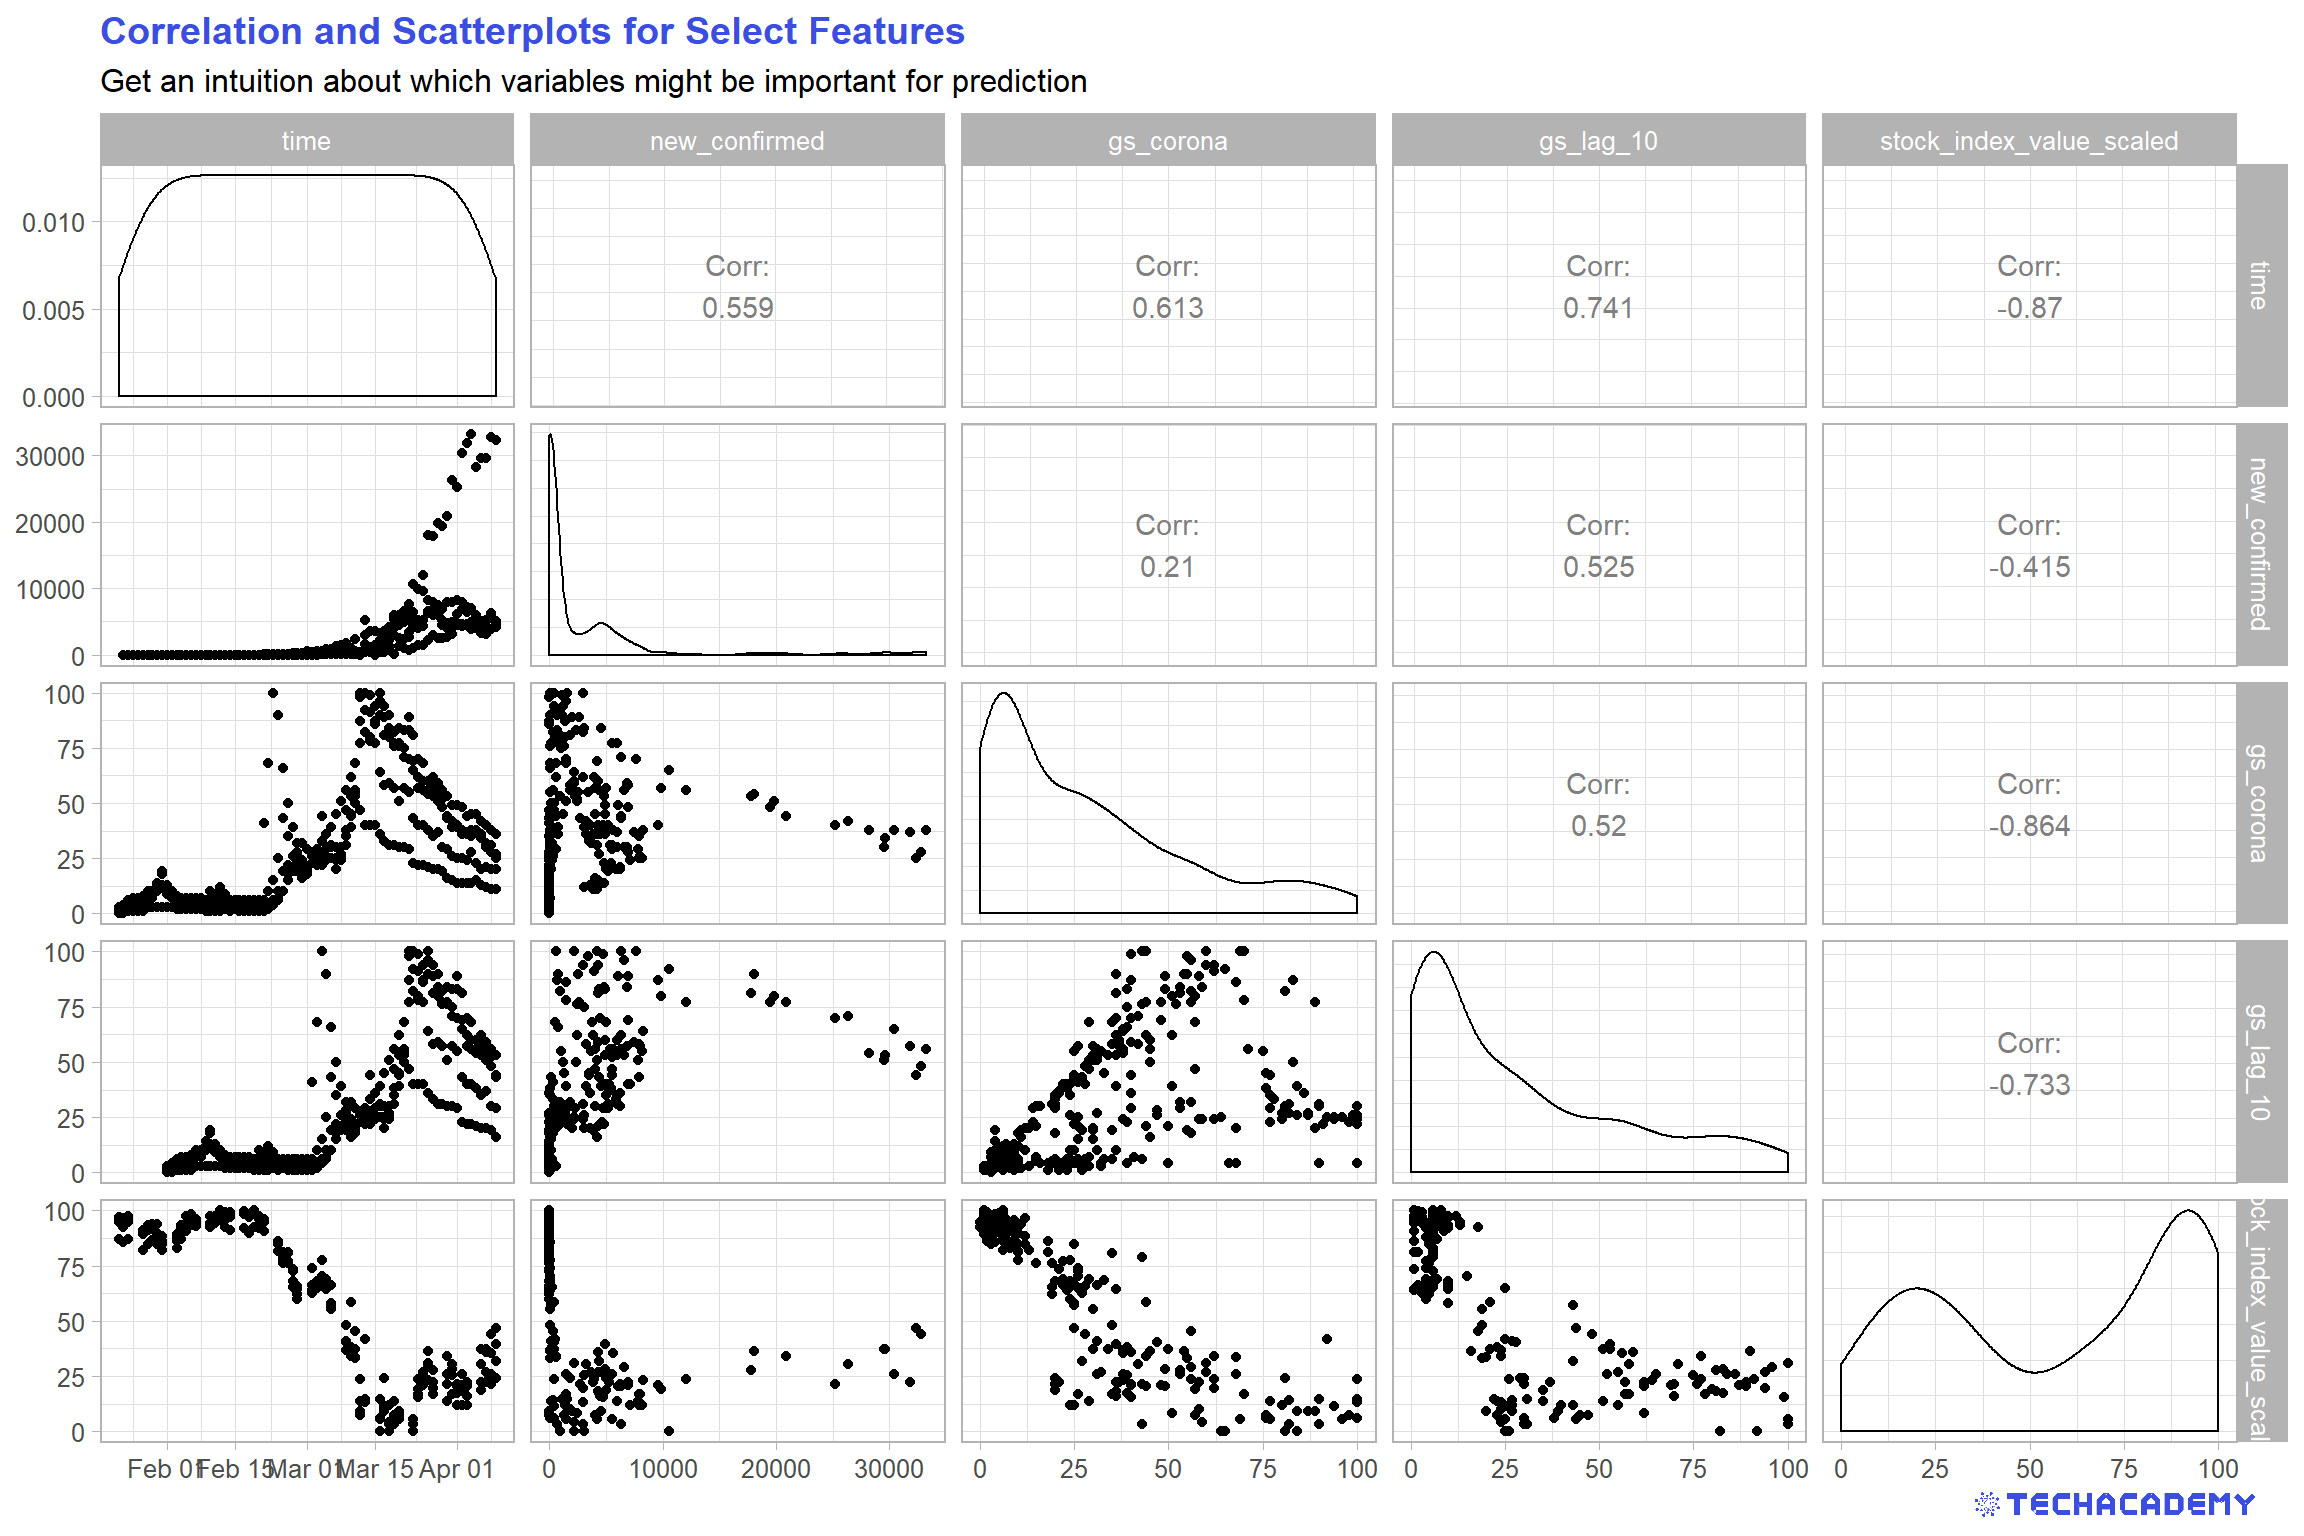
\includegraphics{output_files/figure-latex/unnamed-chunk-33-1.pdf}

\begin{tips}r

Compute the daily number of new infections for each observation in the data set. You can select previous day's values with the \texttt{dplyr} function \texttt{lag()}. Take care of accurately computing the lags over several countries in our data set by grouping your data frame appropriately.

You can either compute ten different lags by just copying and pasting your code. Or you can write a function that takes care of this process automatically. The first option is very error prone and not flexible at all. What if you want to do 15 instead of ten lags? So google how you can automatically create several different lag-variables at once.

Use the function \texttt{cor()} to analyze the correlation between your variables in a correlation matrix. Which features display the highest correlation?

Use the library \texttt{GGally} to generate a nice table that contains both scatterplots and correlations -- but restrict yourself to promising variables. This plot is rather complex and takes increasingly more time to compute and becomes less readable the more variables you include. Maybe stick to the most promising 5 to 7 variables.

\end{tips}

\begin{tipsp}p

You have to compute the \texttt{new\_confirmed} column first, which can easily be done with the pandas function \texttt{df{[}‘column\_name´{]}.diff()}, which computes the difference between the current value of the column and the value of the row before. But keep in mind that you first have to group your data by the different countries in the data frame.
Quite similarly you can compute the lags using the pandas function \texttt{df{[}‘colum\_name’{]}.shift(1)}.

To compute the correlation matrix you can use a function from the seaborn library, which builds on top of matplotlib and is often a useful extension.
Import seaborn using \texttt{import\ seaborn\ as\ sns} and use than the seaborn function \texttt{sns.heatmap(df.corr())}. This function takes as input a pandas data frame on which the pandas function \texttt{corr()} is applied -- which computes the correlations between the different columns. If you compute the correlation heatmap for all columns in the data frame, it can be a bit confusing, therefore select just a subset of all columns.
You can then visualize the correlations in a scatter plot using the seaborn function \texttt{sns.pairplot(df)}, which again takes a data frame as input.

\end{tipsp}

\hypertarget{build-a-simple-model-prototype}{%
\subsection{Build a Simple Model Prototype}\label{build-a-simple-model-prototype}}

If you have a look at the correlation matrix from the last exercise, you notice a correlation between \texttt{new\_confirmed} and \texttt{gs\_corona} of around 0.2. We want to use this data now in our model and evaluate how good this prediction is.
The idea is, that if a lot of people search on the internet for symptoms and the keyword \texttt{corona}, a lot of new infections are to be expected. Conversely, if few people search for the disease, we might expect less new infections. We start with a linear regression which is a simple yet powerful tool. The model will look like this:

\[ new\_confirmed_t = \beta_0 + \beta_1 gs\_corona_t +\epsilon_t \]

\(new\_confirmed\) is your dependent variable that you want to explain by the independent variable(s), in this case \(gs\_corona\) only. To optimally fit a linear line to the data, the ordinary least squares method estimates an intercept \(\beta_0\) and the coefficient(s) \(\beta_k\) for every single independent variable. In our univariate case, this is only \(\beta_1\).

Before we can start with modelling, we have to define our train and test data sets.
We will begin with a prediction for Germany, so filter the data set in a way that it only contains the data from Germany.
Afterwards, divide your data set into a train and test data set based on the time periods shown in Table \ref{tab:reg-table}.

\begin{table}

\caption{\label{tab:reg-table}Train/Test Split}
\centering
\begin{tabular}[t]{lll}
\toprule
DataSet & From & To\\
\midrule
Train & 01 March 2020 & 25 March 2020\\
Test & 26 March 2020 & 09 April 2020\\
\bottomrule
\end{tabular}
\end{table}

Now we are well prepared to start modelling.
Define a linear regression model of the form shown above and train it on your train
data set with \texttt{new\_confirmed} as the value we want to predict and \texttt{gs\_corona} as
the only feature of the model. After our model is trained, we want to try a prediction
with this model.

Now your model has learned the relationship between the number of new infections and google searches in the training period. You can now take this model to the test time period and check how well it performs on previously unseen data.

Use your test data set to feed it into your model and predict the number of new
infections for the test period. At the moment we don't know how well our model
performs. Let's compute the MAPE as described above for our test data set. Compute the MAPE for your model using the predictions of the test set and
the corresponding actual values of \texttt{new\_confirmed}.

Furthermore, we want to visualize the true values for the train and test data
set, as well as the predictions from our model data set for both time periods in one
plot. This is how the plot should look like:

\begin{center}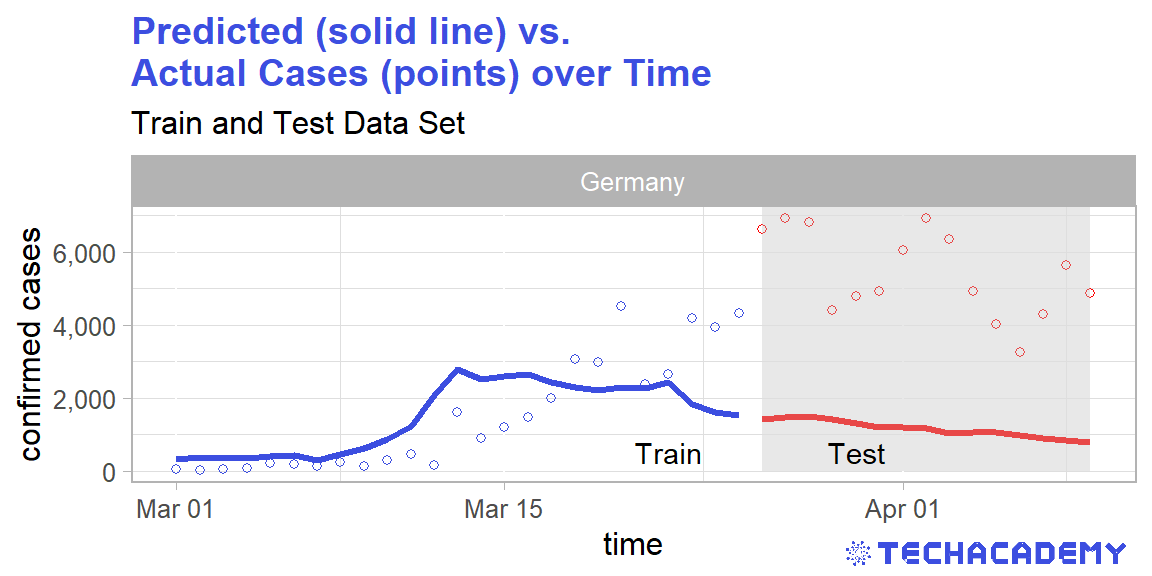
\includegraphics{output_files/figure-latex/unnamed-chunk-36-1} \end{center}

Your first simple linear regression model result might look something like this. Think about what the coefficient and the model fit metrics mean. How good do you think is this model based on the result?

\begin{center}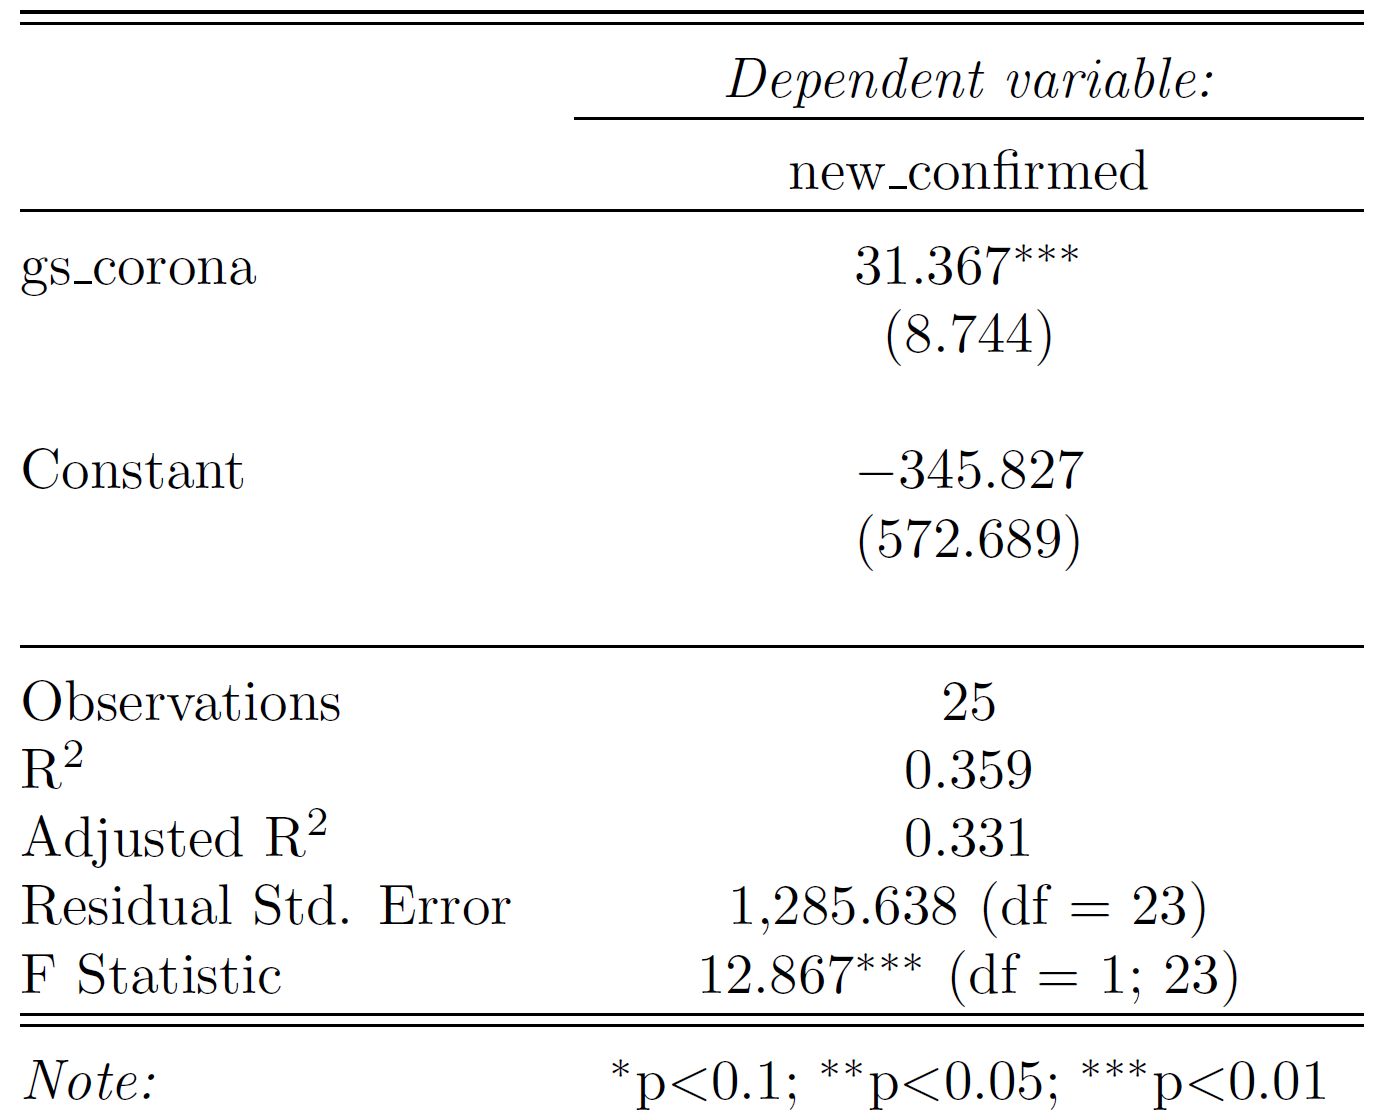
\includegraphics[width=0.5\linewidth]{plots/reg_table} \end{center}

\begin{tips}r

Generate two separate data sets: \texttt{train} and \texttt{test}. Split the original data by time as defined above and select only observations in Germany.

Then use the \texttt{base} function \texttt{lm()} to train the model on your \texttt{train} data set. Save and inspect that model with summary().

Use \texttt{predict()} to apply the model to your test data set. This function returns the predictions \(\hat{y}_t\) as a vector.

It might make sense to name the relevant y-vectors in a structured way. You could think about such a structure:

\texttt{y\_train\_vec}, \texttt{yhat\_train\_vec}, \texttt{y\_test\_vec}, and \texttt{yhat\_test\_vec}, where \texttt{y} refers to the actual values and \texttt{yhat} denotes the predicted values.

You can easily generate regression tables in nice LaTeX, HTML or text format with the package \texttt{stargazer}. Use it to compare different models among each other in your RMarkdown document.

\end{tips}

\begin{tipsp}p

Filter the data correspondingly and you should have for different pandas series:
X\_train = values of \texttt{gs\_corona} in the train period
X\_test = values of \texttt{gs\_corona} in the test period
y\_train = values of \texttt{new\_confirmed} in train period
y\_test = values of \texttt{new\_confirmed} in test period

You have to import \texttt{LinearRegression()} from \texttt{sklear.linear\_model} and can then train your model using
model = LinearRegression()
model.fit(X\_train.reshape(-1,1), y\_train)

You need to reshape the X values because you only use one feature in this case. If you use more then one feature you don't have to reshape your data.
After training, you can use the \texttt{predict()} method on your model an pass the X\_test values to the model.

\end{tipsp}

\hypertarget{refine-your-simple-regression-model}{%
\subsection{Refine Your Simple Regression Model}\label{refine-your-simple-regression-model}}

If you look at the predictions of your model for the train and test period, you see that it doesn't work well, especially on the test period. A possibility could be that there is a lag between the time people google for symptoms to when they are diagnosed with Covid-19. You probably start googling once you show symptoms which is likely a few days before you visit a doctor. After the visit, it will additionally take a few days before your test results will arrive. Therefore we want to include a lag in our model. Luckily we've already computed the lagged values.

Train a new linear regression model, but in this case, don't use the \texttt{gs\_corona} column as a feature, but the column with a lag of ten days. Your model will then have this form:

\[ new\_confirmed_t = \beta_0 + \beta_1 gs\_corona_{t-10} +\epsilon_t \]

Look at the subscript for \(gs\_corona\). That's the only difference to your previous model.

Again compute the MAPE and visualize the prediction as you have done before. You can just reuse most of the code from the previous exercise. Compare the MAPE and your visualization with the model you build before. Did it improve?

Now check out the other features that are available to you in the data set.
Include additional features into your model, for example, stock data or other lagged data. Build several different models and each time evaluate them and compare it with the other models. Do you find models that perform significantly better than the benchmark univariate linear regression model? Keep in mind that you can only reasonably compare a model's performance on previously unseen test data sets.
Always keep visualizing the results, as this is one of the easiest methods to spot how well a model can predict the true values.

Now take your best-performing model in terms of MAPE and based on your visual inspection. Use it for the next exercise.

\hypertarget{extend-your-model-to-several-countries}{%
\subsection{Extend Your Model to Several Countries}\label{extend-your-model-to-several-countries}}

Until now you've trained your model only on data for Germany. Train your model now on several countries on the train data set and evaluate how it performs on both the training and test observations. Do this by computing the MAPE and visualizing your predictions.

Since you have different countries in your models, it might make sense to include a country-variable (dummy) in your regression.

\[new\_confirmed_{it} = \beta_0 + \beta_1 gs\_corona_{it-10} + \beta_3 country_i +\epsilon_{it} \]

A side note, which you can consider in your model, but don't need to: In this model setup, \(\beta_3\) tells you, by how much the number of new confirmed cases deviates from the baseline country, on average in \emph{absolute terms}. This might not make too much sense. Take the example US and Germany. It is likely that those countries do not have a time-stable difference in the absolute number of new confirmed cases. Rather it might be the case that Germany on average has a constant percentage less daily new infections over time than the US. You can incorporate that behaviour into your model by not using the ``level'' of \(new\_confirmed\) but instead using the natural logarithm \(ln(new\_confirmed)\) as the dependent variable. The interpretation for the coefficients now changes. Google how you can interpret the coefficient for the country dummy in this case (hint: ``level-level, log-level regression'').

If you choose to make those transformations, don't forget to transform your predicted values back from the log values to level by exponentiating them.

Again evaluate your model's predictions visually and in terms of MAPE. How well does your model work on other countries than Germany? Try to find reasons for country-specific differences and conclude if you would use such a model to predict the number of new daily infections.

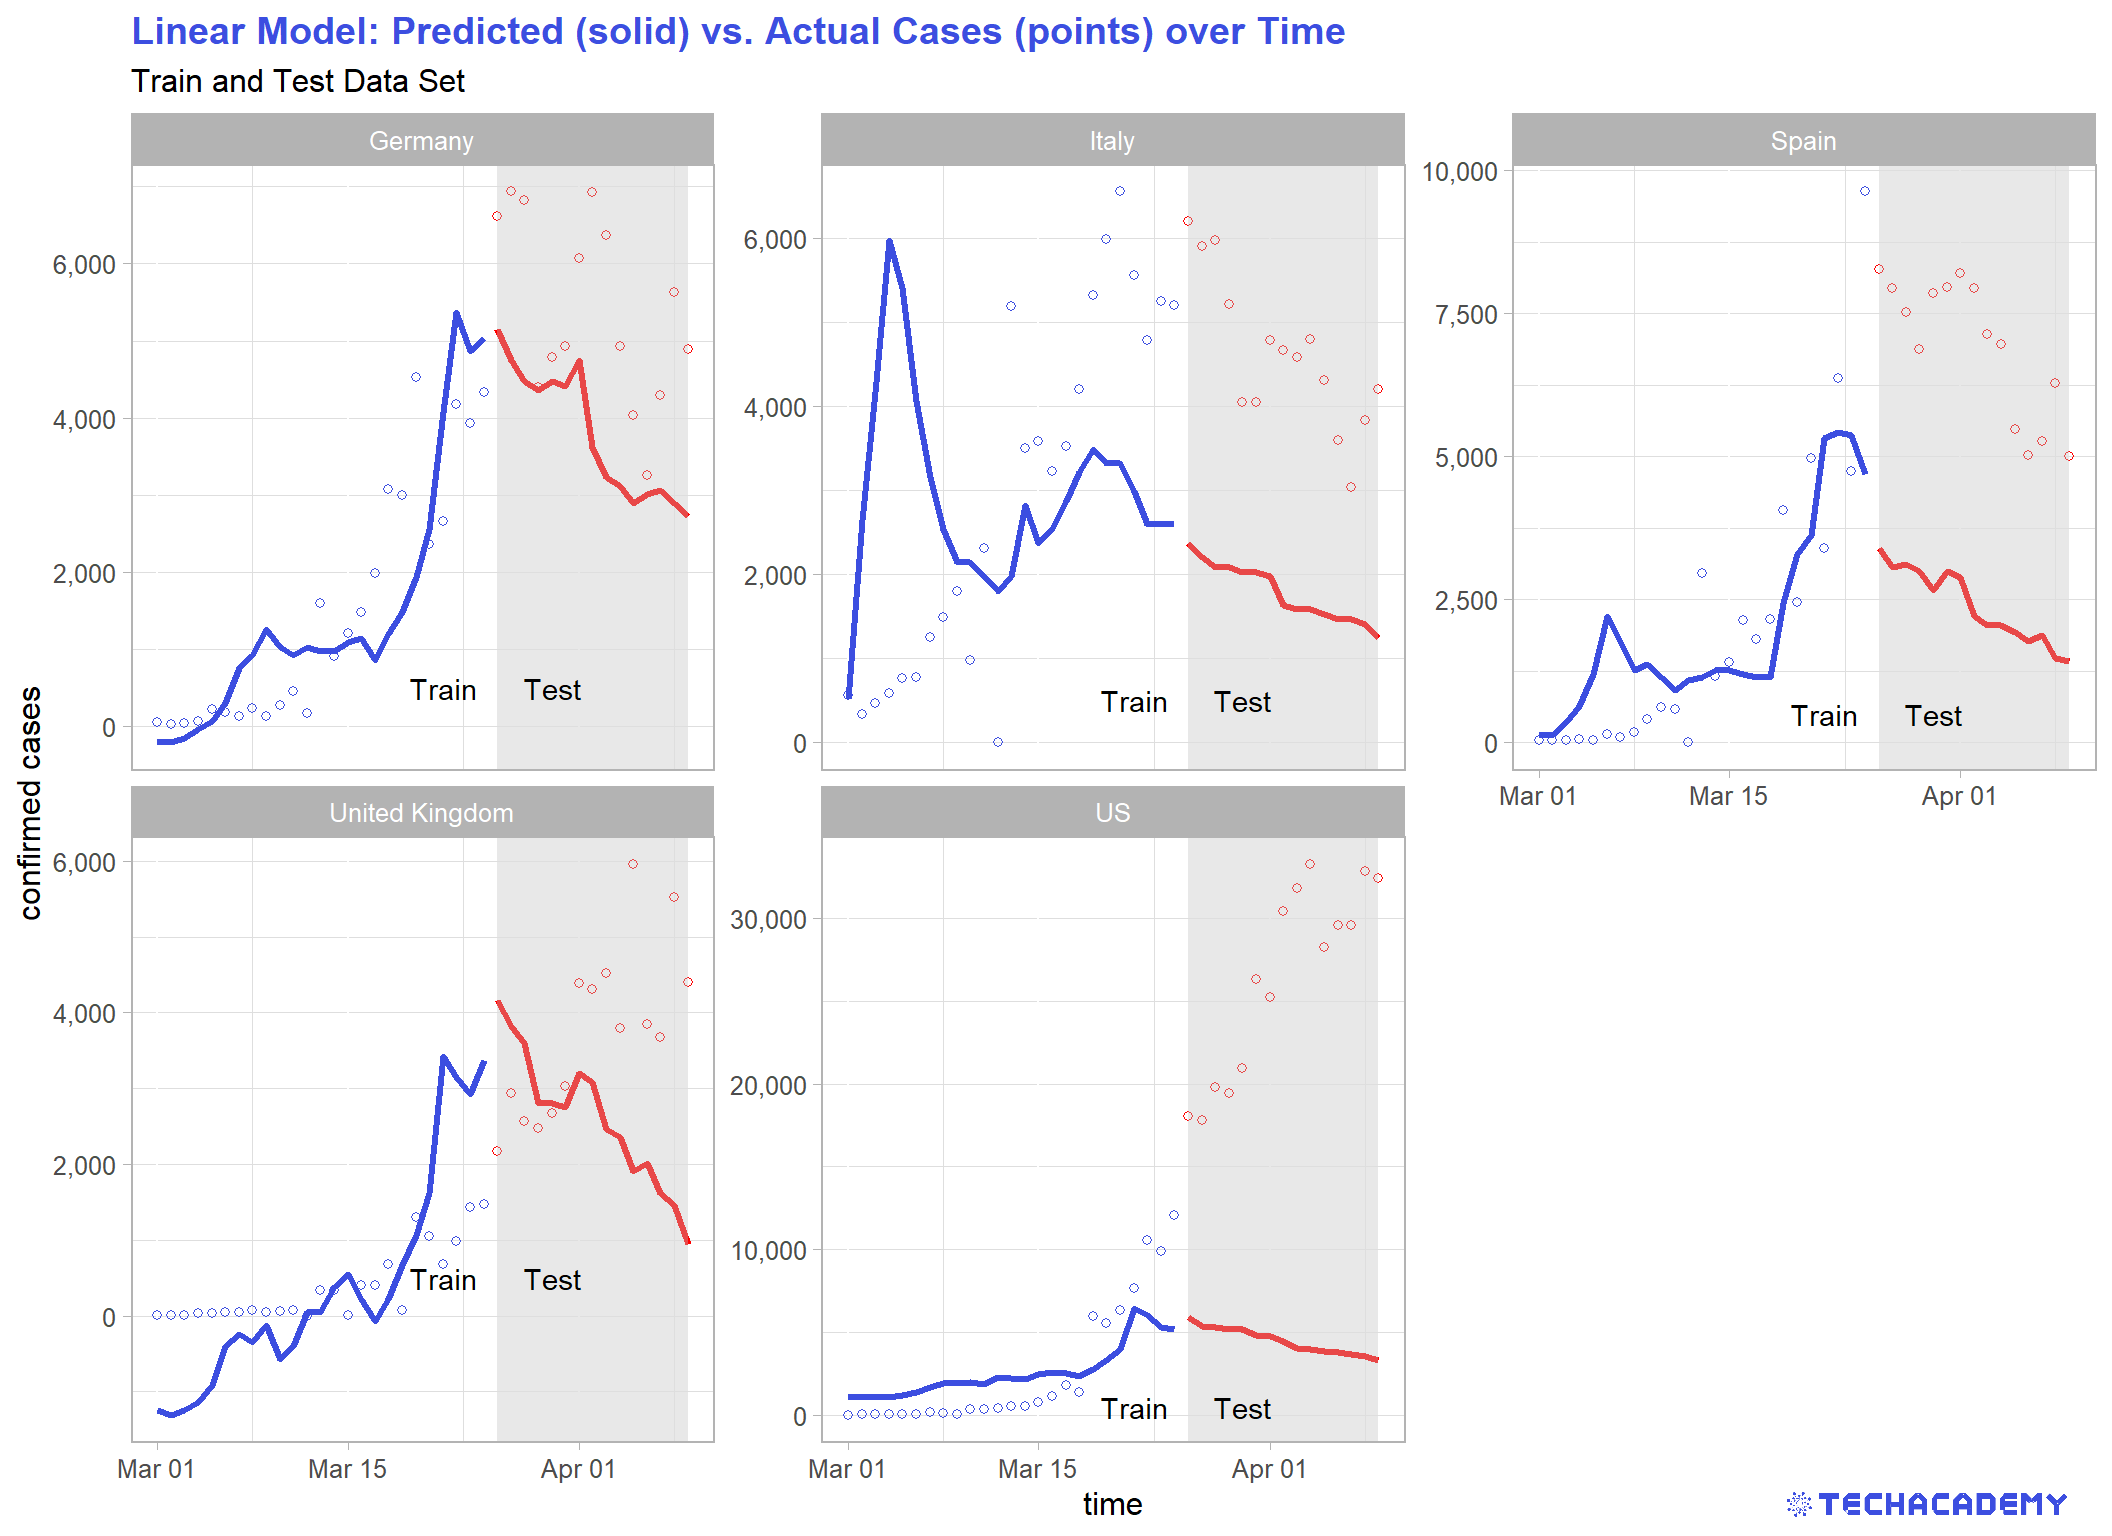
\includegraphics{output_files/figure-latex/unnamed-chunk-40-1.pdf}

Congratulations! You've made it to the end of your TechAcademy Data Science project.
After visualizing the data in the first part, you've also set up predictive models in this section.
If you stuck around until this part and managed to code the better part of the exercises, you've definitely earned your certificate!
We hope you had fun learning Data Science with this data set and you enjoyed it -- at least the parts where you didn't get stuck forever because of some unexplainable coding error.

\newpage

\hypertarget{excercise-checklist}{%
\section{Excercise Checklist}\label{excercise-checklist}}

This checklist should help you keeping track of your exercises. Remember that you have to hand in satisfactory solutions to at least two thirds of the exercises. If you're part of the beginner track this refers to two thirds of part A (EDA) only. If you're part of the advanced track, you have to hand in at least two thirds of both individual parts A and B. Hence, you cannot hand in 100 percent of the first part and only 50 percent of the second one. You'll need more than 66\% in each one for a certificate. After all, you're not really that advanced if you only did half of it, right?

\textbf{Part A: Exploratory Data Analysis (Beginner and Advanced)}

\begin{enumerate}
\def\labelenumi{\arabic{enumi}.}
\tightlist
\item
  Visualize Google Searches

  \begin{itemize}
  \tightlist
  \item
    Change the format of the dates
  \item
    Plot the time series for ``coronavirus'' Google searches
  \item
    Find out what happened on the date the spike occurred
  \end{itemize}
\item
  Visualize the stock market data

  \begin{itemize}
  \tightlist
  \item
    Change the names of the stock symbols
  \item
    Plot the stocks in different panels and add vertical lines
  \end{itemize}
\item
  Covid-19 Visualization

  \begin{itemize}
  \tightlist
  \item
    Create a line plot of the worldwide development of confirmed cases

    \begin{itemize}
    \tightlist
    \item
      Replace missing values with 0
    \item
      Aggregate Data over all countries by time
    \item
      Plot the worldwide time series of confirmed cases
    \item
      Why is there a kink around February 10th?
    \end{itemize}
  \item
    Stacked line plot by country, top 9 countries

    \begin{itemize}
    \tightlist
    \item
      Find countries with the highest number of confirmed cases
    \item
      Plot the stacked line plot
    \end{itemize}
  \item
    Area Plot with new variable \texttt{netinfected}

    \begin{itemize}
    \tightlist
    \item
      Merge the data sets by ID
    \item
      Create new variable \texttt{netinfected}
    \item
      Plot an area plot for the coronavirus variables for each country
    \item
      Create a bar plot with the same measures for each country
    \end{itemize}
  \item
    Bar plot of the Mortality Rate

    \begin{itemize}
    \tightlist
    \item
      Create a new variable ``mortality rate'' with a measure of your choice
    \item
      Select the 35 countries with the highest mortality rate
    \item
      Create a bar plot of the mortality rate of those countries
    \item
      Highlight the countries with the highest number of confirmed cases
    \item
      How can you explain the difference in the mortality rate for the top 5 countries?
    \item
      Do you see an issue with how you calculated the mortality rate? How would you measure the mortality rate if you had all the resources you needed?
    \end{itemize}
  \item
    Visualization with Maps (depends on R/Python: Check the boxes in the exercise for exact tasks)
  \end{itemize}
\end{enumerate}

\textbf{Part B: COVID-19 Predictions (Advanced)}

\begin{enumerate}
\def\labelenumi{\arabic{enumi}.}
\tightlist
\item
  Feature Engineering and Correlation Analysis

  \begin{itemize}
  \tightlist
  \item
    Generate ``New Confirmed'' variable
  \item
    Generate lag(GoogleSearch) (0-10)
  \item
    Generate correlation matrix
  \item
    Visualize relationships in e.g.~scatterplots
  \end{itemize}
\item
  Build a Simple Model Prototype

  \begin{itemize}
  \tightlist
  \item
    Filter Germany only
  \item
    Generate train/test split by date
  \item
    Set up simple univariate linear regression
  \item
    Calculate model performance (MAPE)
  \item
    Plot \(y_{it}\) and \(\hat{y}_{it}\) vs.~time in one plot and visualize train/test split
  \end{itemize}
\item
  Refine Your Simple Regression Model

  \begin{itemize}
  \tightlist
  \item
    Again same observations as above, but use lag(GoogleSearch) as independent variable
  \item
    Compare model performance (MAPE and visually) to the current Google Search Variable without lag
  \item
    Try other features and check if they increase performance
  \end{itemize}
\item
  Extend Your Model to Several Countries

  \begin{itemize}
  \tightlist
  \item
    Pick your best model and train and test it on the entire data set with several countries
  \item
    Evaluate model performance (MAPE and visually)
  \item
    Find reasons why country-specific differences exist and outline if your approach is viable
  \end{itemize}
\end{enumerate}

\newpage

\hypertarget{whats-next-in-your-data-science-career}{%
\section{What's Next in Your Data Science Career?}\label{whats-next-in-your-data-science-career}}

At the end of your TechAcademy semester, you've successfully coded your way through a whole Data Science project. You liked what you did and would like bring your skills to the next level? Then this section provides you with many useful resources to deepen your knowledge in Data Science in general or Python and R in particular. The first section is useful for every aspiring Data Scientist, while the two following boxes introduce you to some language-specific resources. If you've come across some other useful materials that we didn't mention here, feel free to contact us -- this list is far from complete!

\hypertarget{data-science-in-general}{%
\subsection{Data Science in General}\label{data-science-in-general}}

\hypertarget{version-control-with-git}{%
\paragraph*{\texorpdfstring{Version Control with \href{https://github.com/}{Git}}{Version Control with Git}}\label{version-control-with-git}}
\addcontentsline{toc}{paragraph}{Version Control with \href{https://github.com/}{Git}}

If you're serious about data science, you will need Git. Better learn it early and start enjoying and appreciating it before it's too late and you're pressured into learning it on the fly! Every project you do should be versioned with Git. Regardless if you're working alone or with a big group of developers. Regardless if you write ten lines of code or a really complex program. With Git, you can keep track of all your changes. It's like a Dropbox/Google Drive for developers, but way better. Pro-Tip: Get free GitHub Pro as a Student with the \href{https://education.github.com/pack}{GitHub Student Developer Pack}. Besides all the perks of GitHub Pro, you'll also free access to many other great tools. See the respective tutorials on how to set up your Git workflow.

\hypertarget{advice-for-non-traditional-data-scientists}{%
\paragraph*{\texorpdfstring{Advice for \href{https://blog.shotwell.ca/posts/learning_data_science/}{Non-Traditional Data Scientists}}{Advice for Non-Traditional Data Scientists}}\label{advice-for-non-traditional-data-scientists}}
\addcontentsline{toc}{paragraph}{Advice for \href{https://blog.shotwell.ca/posts/learning_data_science/}{Non-Traditional Data Scientists}}

Important advice from Gordon Shotwell, a former lawyer, on what it takes to have a successful data science career coming from a non-computer science background. Extremely encouraging and helpful read on what you should and shouldn't do to reach that goal.

\hypertarget{learn-from-great-data-scientists-on-kaggle}{%
\paragraph*{\texorpdfstring{Learn from Great Data Scientists on \href{https://www.kaggle.com/}{Kaggle}}{Learn from Great Data Scientists on Kaggle}}\label{learn-from-great-data-scientists-on-kaggle}}
\addcontentsline{toc}{paragraph}{Learn from Great Data Scientists on \href{https://www.kaggle.com/}{Kaggle}}

Kaggle is a platform that hosts data science challenges. The great thing about it is that you can browse through many clever solutions to tricky machine learning tasks. And of course, you can also join the competition and measure your predictions with others. There are plenty of both Python and R notebooks.

\hypertarget{r}{%
\subsection{R}\label{r}}

\begin{tips}r

\textbf{Install R and RStudio Locally}

RStudio.Cloud is great for getting started with R without having to worry about installing anything locally. Sooner or later you will have to install everything on your own computer. Here's a \href{https://www.datacamp.com/community/tutorials/installing-R-windows-mac-ubuntu}{DataCamp tutorial} on how to do that.

\textbf{Version Control with Git}

RStudio has a nice interface that lets you enjoy the perks of Git without ever having to touch the command line -- sounds great, does it? Learn how to set up the Git \& R workflow with \href{https://happygitwithr.com/}{Happy Git with R}.

\textbf{\href{https://www.r-graph-gallery.com/}{R Graph Gallery}}

Get inspiration to take your plotting to the next level. Includes code to reproduce the plots.

\textbf{Follow the R Master Himself and the R Community}

Hadley Wickham was and continues to be extremely influential on the development of R and its rise to one of the most popular data science languages. He's behind many tools that we taught you in this semester, especially the tidyverse (including great packages such as ggplot2 and dplyr). Follow him \href{https://twitter.com/hadleywickham}{on Twitter} to get great R advice and keep up to speed with everything new to R. Following the many people behind R (not only Hadley) is a great way for acquiring deeper understanding of the language and its developments.

\textbf{Join the \href{https://www.meetup.com/r-frankfurt/}{Campus useR Group in Frankfurt}}

There's a quite active R community in Frankfurt that meets once a month. It's open for students, professors, industry practitioners, journalists, and all people that love to use R. In those meetings, you'll hear about other's work, discuss new developments, and ask questions.

\textbf{Listen to R Podcasts}
Another great way to easily keep up with new developments in the Data Science/R community. Check out
\href{http://nssdeviations.com/}{Not So Standard Deviations} or \href{https://r-podcast.org/}{the R-Podcast}

\end{tips}

\hypertarget{python}{%
\subsection{Python}\label{python}}

\begin{tipsp}p

\textbf{Install Python Locally}

Until now you've only programmed using JupyterHub on the TechAcademy Server. A next step would be to install Python and Jupyter locally on your computer. This \href{https://docs.anaconda.com/anaconda/install/}{link} contains the necessary information on how to install the software on Windows, iOS or Linux.

\textbf{Choosing the Right Editor}

Using Jupyter is especially useful for short data analyses. But sometimes you want to write longer scripts in Python. In these cases, it is often more convenient to use a code editor instead of Jupyter. \href{https://realpython.com/learning-paths/perfect-your-python-development-setup/}{This tutorial} highlights the positive aspects of such an editor and how to choose the right one for you. Pro Tip: Also check out the other tutorials on \href{https://realpython.com/}{Real Python}.

\textbf{\href{https://python-graph-gallery.com/}{Python Graph Gallery}}

Get inspiration to take your plotting to the next level. Includes code to reproduce the plots.

\textbf{More Advanced Python Concepts}

You know the basic data structures in Python like lists and dictionaries. What are the next steps to improve your knowledge? \href{https://book.pythontips.com/en/latest/index.html}{This website} gives good explanations for slightly more advanced concepts which can be very useful from time to time.

\textbf{A Deeper Understanding}

If you want to get a deeper understanding of the Python programming language and into typical algorithms which are used in the field of Data Science, this \href{https://github.com/ab-anand/py-books/blob/master/Data\%20Science\%20from\%20Scratch-\%20First\%20Principles\%20with\%20Python.pdf}{free book} can be a good starting point.

\textbf{Writing Beautiful Python Code}

``My code doesn't look nice, but it works!''
This might work for yourself, but often you will work on code with other people. But even if you're just coding for yourself it's a good idea to follow the PEP8 style guide. It's a useful convention on how to structure and code in Python. You'll find useful resources for PEP8 \href{https://realpython.com/python-pep8/}{here} and \href{https://www.python.org/dev/peps/pep-0020/\#id2}{here}.

\textbf{Listen to Python Podcasts}

When you don't have time for books you can listen to \href{https://talkpython.fm/home}{Talk Python} or the \href{https://www.pythonpodcast.com}{Python Podcast}.

\end{tipsp}

  \bibliography{book.bib,packages.bib}

\end{document}
